%% ============================================================
%% PARTE III — EXERCÍCIOS KUMON: FOLHAS DE PRÁTICA COMPLETAS
%% ============================================================
%% Volume 1 — Alfabetização (1º Ano do Ensino Fundamental)
%% Progressão: Pré-silábico -> Silábico -> Silábico-Alfabético
%%
%% Estrutura de cada folha:
%%   PARTE 1: RECONHECIMENTO (5 itens)
%%   PARTE 2: PRODUÇÃO GUIADA (5 itens)
%%   PARTE 3: INTEGRAÇÃO (5 itens)
%%   Total por folha: 15 itens
%%
%% Normas aplicadas:
%%   - BNCC: EF01LP01 a EF01LP09
%%   - CAEd: D1 (palavras), D2 (frases), D3 (textos),
%%           D4 (produção), D5 (gramática)
%%   - SPAECE: EF01LP01-EF01LP09
%%   - DCNC: Resolução CNE/CEB nº 2/2012
%% ============================================================

\chapter{Exercícios Kumon --- Folhas de Prática}

\section{Princípios dos Exercícios Kumon}

Os exercícios Kumon seguem a progressão rigorosa do método japonês, adaptada
para a alfabetização em língua portuguesa:

\begin{enumerate}[leftmargin=2cm]
  \item \textbf{Reconhecimento}: O aluno identifica a letra, sílaba ou
        palavra em diferentes contextos visuais e auditivos.
  \item \textbf{Produção guiada}: O aluno completa, copia ou escreve a
        letra/sílaba com apoio estruturado.
  \item \textbf{Integração}: O aluno usa a letra/sílaba em palavras,
        frases e textos completos, demonstrando compreensão.
  \item \textbf{Fluência}: O aluno lê e escreve com velocidade e precisão
        crescentes (meta de tempo por folha).
\end{enumerate}

\textbf{Regras de Progressão:}
\begin{enumerate}[leftmargin=2cm]
  \item O aluno só avança quando atingir 90\% de acerto na folha atual.
  \item Erros são revisados com exercícios intermediários.
  \item A velocidade aumenta gradualmente (meta de tempo por folha).
  \item Revisão semanal consolida os conteúdos aprendidos.
  \item O professor registra o desempenho no caderno de acompanhamento.
\end{enumerate}

\textbf{Código de Correção:}
\begin{center}
\begin{tabular}{|c|c|c|}
\hline
$\checkmark$ (verde) & $\triangle$ (amarelo) & $\times$ (vermelho) \\
\hline
12--15 acertos & 8--11 acertos & Menos de 8 acertos \\
Reforço positivo & Reforço & Reforço intensivo \\
\hline
\end{tabular}
\end{center}

%% ============================================================
%% TABELA DE PROGRESSÃO KUMON
%% ============================================================
\subsection{Progressão Kumon --- Níveis de Leitura}

\kumonprogression

\textbf{Observação:} Este Volume 1 cobre os níveis 7A a 4A do Kumon Reading
program, adaptados para o contexto brasileiro. Cada folha de prática segue
a estrutura Kumon: Reconhecimento (5 itens) → Produção Guiada (5 itens) →
Integração (5 itens) = 15 itens por folha.

%% ============================================================
%% DESCRITORES SPAECE-ALFA
%% ============================================================
\subsection{Descritores SPAECE-Alfa (Avaliação de Alfabetização)}

\spaecealfa

%% ============================================================
%% 6 COMPONENTES DA PNA
%% ============================================================
\subsection{6 Componentes da Política Nacional de Alfabetização (PNA)}

\pnacomponents

\textbf{Integração nos exercícios:} Cada folha de prática Kumon integra
mínimo 4 dos 6 componentes da PNA, garantindo que o aluno desenvolva
consciência fonêmica, instrução fônica sistemática, fluência e produção
de escrita simultaneamente.

%% ============================================================
%% SEÇÃO 1: VOGAIS — PRÉ-SILÁBICO
%% ============================================================

\section{Folhas de Prática --- Vogais (Pré-silábico)}

% FOLHA A-01: LETRA A

\plancheta{Folha A-01 --- Letra A}
\subsection{Folha A-01 --- Letra A}

\begin{exercicio}[Folha de Prática A-01 --- Letra A]
\metadata{A-01}{Pré-silábico}{EF01LP01}{D1}{EF01LP01}{CNE/CEB nº 2/2012}
\kumontiming{1}{90}

\noindent\textbf{Nome:} \underline{\hspace{4cm}} \quad \textbf{Nota:} \underline{\hspace{1cm}}/15

\subsection*{PARTE 1: RECONHECIMENTO (5 itens)}

\begin{enumerate}
  \item \textbf{Circular a letra A'' em meio a outras letras:}
  \begin{center}
  A \quad B \quad \textbf{A} \quad C \quad D \quad \textbf{A} \quad E \quad \textbf{A} \quad F \quad G
  \end{center}

  \item \textbf{Sublinhar todas as palavras que começam com A'':}
  \begin{center}
  \uline{água} \quad bola \quad \uline{avião} \quad sapo \quad \uline{abacaxi} \quad gato \quad \uline{arco}
  \end{center}

  \item \textbf{Identificar a letra A'' nas palavras abaixo:}
  \begin{center}
  avião $\rightarrow$ A está na posição \underline{\hspace{1cm}} \\
  água $\rightarrow$ A está na posição \underline{\hspace{1cm}} \\
  amarelo $\rightarrow$ A está na posição \underline{\hspace{1cm}}
  \end{center}

  \item \textbf{Dizer em voz alta cada letra e apontar para a A'':}
  \begin{center}
  A \quad B \quad C \quad \textbf{A} \quad D \quad E \quad F \quad \textbf{A} \quad G \quad H
  \end{center}

  \item \textbf{Contar quantas vezes a letra A'' aparece:}
  \begin{center}
  AMARELO $\rightarrow$ quantas A''? \underline{\hspace{1cm}} \\
  AVIÃO $\rightarrow$ quantas A''? \underline{\hspace{1cm}} \\
  ÁGUA $\rightarrow$ quantas A''? \underline{\hspace{1cm}}
  \end{center}
\end{enumerate}

\subsection*{PARTE 2: PRODUÇÃO GUIADA (5 itens)}

\begin{enumerate}[resume]
  \item \textbf{Copiar a letra A'' cinco vezes:}
  \begin{center}
  A \quad \underline{\hspace{1.5cm}} \quad \underline{\hspace{1.5cm}} \quad \underline{\hspace{1.5cm}} \quad \underline{\hspace{1.5cm}} \quad \underline{\hspace{1.5cm}}
  \end{center}

  \item \textbf{Completar as palavras com a letra A'':}
  \begin{center}
  \underline{A}vião \quad \underline{A}gua \quad \underline{A}bacaxi \quad \underline{A}marelo \quad \underline{A}rco
  \end{center}

  \item \textbf{Escrever a letra A'' maiúscula e minúscula:}
  \begin{center}
  Maiúscula: \underline{\hspace{2cm}} \quad Minúscula: \underline{\hspace{2cm}}
  \end{center}

  \item \textbf{Traçar a letra A'' e copiar:}
  \begin{center}
  \begin{tikzpicture}
    \draw[thick, dashed] (0,0) -- (0,1.5) -- (1,3);
    \draw[thick, dashed] (1,3) -- (2,1.5) -- (2,0);
    \draw[thick, dashed] (0.3,1.8) -- (1.7,1.8);
  \end{tikzpicture}
  \end{center}

  \item \textbf{Escrever 3 palavras que começam com A'':}
  \begin{center}
  1. \underline{\hspace{3cm}} \quad 2. \underline{\hspace{3cm}} \quad 3. \underline{\hspace{3cm}}
  \end{center}
\end{enumerate}

\subsection*{PARTE 3: INTEGRAÇÃO (5 itens)}

\begin{enumerate}[resume]
  \item \textbf{Ler em voz alta as palavras abaixo:}
  \begin{center}
  $\rightarrow$ ÁGUA  ~  AVIÃO  ~  ABACAXI  ~  AMARELO  ~  ARCO
  \end{center}

  \item \textbf{Ligar a palavra à figura correspondente:}
  \begin{center}
  \begin{tabular}{cc}
  AVIÃO & \quad --- \quad $\square$ \\
  ÁGUA & \quad --- \quad $\square$ \\
  ARCO & \quad --- \quad $\square$
  \end{tabular}
  \end{center}

  \item \textbf{Ler a frase e desenhar o que ela diz:}
  \begin{center}
  $\rightarrow$ O avião é amarelo.
  \end{center}
  \begin{center}
  \begin{tikzpicture}
    \draw[thick, dashed] (0,0) rectangle (6,3);
  \end{tikzpicture}
  \end{center}

  \item \textbf{Completar a frase com A'':}
  \begin{center}
  O p\underline{~~~}vo \quad A m\underline{~~~}ça \quad O avi\underline{~~~}o
  \end{center}

  \item \textbf{Escrever uma frase usando pelo menos uma palavra com A'':}
  \begin{center}
  \underline{\hspace{12cm}} \\
  \underline{\hspace{12cm}}
  \end{center}
\end{enumerate}

\noindent\textbf{NOTA:} \underline{\hspace{1cm}}/15 \quad $\checkmark$ = 12--15 \quad $\triangle$ = 8--11 \quad $\times$ = menos de 8
\end{exercicio}

\begin{somletra}[title={\faMusic~Atividade de Som da Vogal --- B\^onus (n\~ao vale nota)}]
\textbf{1. Ca\c{c}a ao som.} Marque as palavras que t\^e{}m o som de A:
\begin{center}
$\square$~ABELHA \quad $\square$~BOLA \quad $\square$~AVI\~AO \quad $\square$~DEDO \quad $\square$~CASA \quad $\square$~P\'E
\end{center}

\textbf{2. Tem ou n\~ao{} tem?} Rodeie SIM ou N\~ao:
\begin{center}
ABELHA --- (\textbf{SIM}) (\textbf{N\~AO}) \quad BOLA --- (\textbf{SIM}) (\textbf{N\~AO}) \\ AVI\~AO --- (\textbf{SIM}) (\textbf{N\~AO}) \quad DEDO --- (\textbf{SIM}) (\textbf{N\~AO})
\end{center}
\caixapausa{A boca abre para o som de A.}
\caixapista{A vogal A aparece na s\'ilaba forte e na fraca.}
\end{somletra}

% bonus_R205_A-01

% FOLHA A-02: LETRA E

\plancheta{Folha A-02 --- Letra E}
\subsection{Folha A-02 --- Letra E}

\begin{exercicio}[Folha de Prática A-02 --- Letra E]
\metadata{A-02}{Pré-silábico}{EF01LP01}{D1}{EF01LP01}{CNE/CEB nº 2/2012}
\kumontiming{1}{90}

\noindent\textbf{Nome:} \underline{\hspace{4cm}} \quad \textbf{Nota:} \underline{\hspace{1cm}}/15

\subsection*{PARTE 1: RECONHECIMENTO (5 itens)}

\begin{enumerate}
  \item \textbf{Circular a letra E'' em meio a outras letras:}
  \begin{center}
  E \quad F \quad \textbf{E} \quad G \quad H \quad \textbf{E} \quad I \quad J \quad \textbf{E} \quad K
  \end{center}

  \item \textbf{Sublinhar todas as palavras que começam com E'':}
  \begin{center}
  \uline{elefante} \quad gato \quad \uline{escada} \quad sapo \quad \uline{escola} \quad bola \quad \uline{estrela}
  \end{center}

  \item \textbf{Identificar a letra E'' nas palavras abaixo:}
  \begin{center}
  elefante $\rightarrow$ E está na posição \underline{\hspace{1cm}} \\
  escada $\rightarrow$ E está na posição \underline{\hspace{1cm}} \\
  escola $\rightarrow$ E está na posição \underline{\hspace{1cm}}
  \end{center}

  \item \textbf{Dizer em voz alta cada letra e apontar para a E'':}
  \begin{center}
  D \quad \textbf{E} \quad F \quad G \quad \textbf{E} \quad H \quad I \quad J \quad \textbf{E} \quad K
  \end{center}

  \item \textbf{Contar quantas vezes a letra E'' aparece:}
  \begin{center}
  ELEFANTE $\rightarrow$ quantas E''? \underline{\hspace{1cm}} \\
  ESCOLA $\rightarrow$ quantas E''? \underline{\hspace{1cm}} \\
  ESTRELA $\rightarrow$ quantas E''? \underline{\hspace{1cm}}
  \end{center}
\end{enumerate}

\subsection*{PARTE 2: PRODUÇÃO GUIADA (5 itens)}

\begin{enumerate}[resume]
  \item \textbf{Copiar a letra E'' cinco vezes:}
  \begin{center}
  E \quad \underline{\hspace{1.5cm}} \quad \underline{\hspace{1.5cm}} \quad \underline{\hspace{1.5cm}} \quad \underline{\hspace{1.5cm}} \quad \underline{\hspace{1.5cm}}
  \end{center}

  \item \textbf{Completar as palavras com a letra E'':}
  \begin{center}
  \underline{E}lefante \quad \underline{E}scola \quad \underline{E}scada \quad \underline{E}strela \quad \underline{E}spada
  \end{center}

  \item \textbf{Escrever a letra E'' maiúscula e minúscula:}
  \begin{center}
  Maiúscula: \underline{\hspace{2cm}} \quad Minúscula: \underline{\hspace{2cm}}
  \end{center}

  \item \textbf{Traçar a letra E'' e copiar:}
  \begin{center}
  \begin{tikzpicture}
    \draw[thick, dashed] (0,0) -- (0,3);
    \draw[thick, dashed] (0,3) -- (1.5,3);
    \draw[thick, dashed] (0,1.5) -- (1,1.5);
    \draw[thick, dashed] (0,0) -- (1.5,0);
  \end{tikzpicture}
  \end{center}

  \item \textbf{Escrever 3 palavras que começam com E'':}
  \begin{center}
  1. \underline{\hspace{3cm}} \quad 2. \underline{\hspace{3cm}} \quad 3. \underline{\hspace{3cm}}
  \end{center}
\end{enumerate}

\subsection*{PARTE 3: INTEGRAÇÃO (5 itens)}

\begin{enumerate}[resume]
  \item \textbf{Ler em voz alta as palavras abaixo:}
  \begin{center}
  $\rightarrow$ ELEFANTE  ~  ESCOLA  ~  ESCADA  ~  ESTRELA  ~  ESPADA
  \end{center}

  \item \textbf{Ligar a palavra à figura correspondente:}
  \begin{center}
  \begin{tabular}{cc}
  ELEFANTE & \quad --- \quad $\square$ \\
  ESCOLA & \quad --- \quad $\square$ \\
  ESTRELA & \quad --- \quad $\square$
  \end{tabular}
  \end{center}

  \item \textbf{Ler a frase e desenhar o que ela diz:}
  \begin{center}
  $\rightarrow$ O elefante é grande.
  \end{center}
  \begin{center}
  \begin{tikzpicture}
    \draw[thick, dashed] (0,0) rectangle (6,3);
  \end{tikzpicture}
  \end{center}

  \item \textbf{Completar a frase com E'':}
  \begin{center}
  A m\underline{~~~}sa \quad O el\underline{~~~}fante \quad A esc\underline{~~~}la
  \end{center}

  \item \textbf{Escrever uma frase usando pelo menos uma palavra com E'':}
  \begin{center}
  \underline{\hspace{12cm}} \\
  \underline{\hspace{12cm}}
  \end{center}
\end{enumerate}

\noindent\textbf{NOTA:} \underline{\hspace{1cm}}/15 \quad $\checkmark$ = 12--15 \quad $\triangle$ = 8--11 \quad $\times$ = menos de 8
\end{exercicio}

\begin{somletra}[title={\faMusic~Atividade de Som da Vogal --- B\^onus (n\~ao vale nota)}]
\textbf{1. Ca\c{c}a ao som.} Marque as palavras que t\^e{}m o som de E:
\begin{center}
$\square$~ESCOLA \quad $\square$~BOLA \quad $\square$~ELEFANTE \quad $\square$~LUVA \quad $\square$~CEDO \quad $\square$~P\'E
\end{center}

\textbf{2. Tem ou n\~ao{} tem?} Rodeie SIM ou N\~ao:
\begin{center}
ESCOLA --- (\textbf{SIM}) (\textbf{N\~AO}) \quad BOLA --- (\textbf{SIM}) (\textbf{N\~AO}) \\ ELEFANTE --- (\textbf{SIM}) (\textbf{N\~AO}) \quad LUVA --- (\textbf{SIM}) (\textbf{N\~AO})
\end{center}
\caixapausa{A boca faz sorriso para o som de E.}
\caixapista{A vogal E aparece na s\'ilaba forte e na fraca.}
\end{somletra}

% bonus_R205_A-02

% FOLHA A-03: LETRA I

\plancheta{Folha A-03 --- Letra I}
\subsection{Folha A-03 --- Letra I}

\begin{exercicio}[Folha de Prática A-03 --- Letra I]
\metadata{A-03}{Pré-silábico}{EF01LP01}{D1}{EF01LP01}{CNE/CEB nº 2/2012}
\kumontiming{1}{90}

\noindent\textbf{Nome:} \underline{\hspace{4cm}} \quad \textbf{Nota:} \underline{\hspace{1cm}}/15

\subsection*{PARTE 1: RECONHECIMENTO (5 itens)}

\begin{enumerate}
  \item \textbf{Circular a letra I'' em meio a outras letras:}
  \begin{center}
  H \quad I \quad \textbf{I} \quad J \quad K \quad L \quad \textbf{I} \quad M \quad N \quad \textbf{I}
  \end{center}

  \item \textbf{Sublinhar todas as palavras que começam com I'':}
  \begin{center}
  \uline{igreja} \quad bola \quad \uline{ilha} \quad sapo \quad \uline{impressão} \quad gato \quad \uline{interesse}
  \end{center}

  \item \textbf{Identificar a letra I'' nas palavras abaixo:}
  \begin{center}
  igreja $\rightarrow$ I está na posição \underline{\hspace{1cm}} \\
  ilha $\rightarrow$ I está na posição \underline{\hspace{1cm}} \\
  inicial $\rightarrow$ I está na posição \underline{\hspace{1cm}}
  \end{center}

  \item \textbf{Dizer em voz alta cada letra e apontar para a I'':}
  \begin{center}
  G \quad \textbf{I} \quad H \quad J \quad \textbf{I} \quad K \quad L \quad M \quad \textbf{I} \quad N
  \end{center}

  \item \textbf{Contar quantas vezes a letra I'' aparece:}
  \begin{center}
  IGREJA $\rightarrow$ quantas I''? \underline{\hspace{1cm}} \\
  ILHA $\rightarrow$ quantas I''? \underline{\hspace{1cm}} \\
  IMPRESSÃO $\rightarrow$ quantas I''? \underline{\hspace{1cm}}
  \end{center}
\end{enumerate}

\subsection*{PARTE 2: PRODUÇÃO GUIADA (5 itens)}

\begin{enumerate}[resume]
  \item \textbf{Copiar a letra I'' cinco vezes:}
  \begin{center}
  I \quad \underline{\hspace{1.5cm}} \quad \underline{\hspace{1.5cm}} \quad \underline{\hspace{1.5cm}} \quad \underline{\hspace{1.5cm}} \quad \underline{\hspace{1.5cm}}
  \end{center}

  \item \textbf{Completar as palavras com a letra I'':}
  \begin{center}
  \underline{I}greja \quad \underline{I}lha \quad \underline{I}mpressão \quad \underline{I}nício \quad \underline{I}dentidade
  \end{center}

  \item \textbf{Escrever a letra I'' maiúscula e minúscula:}
  \begin{center}
  Maiúscula: \underline{\hspace{2cm}} \quad Minúscula: \underline{\hspace{2cm}}
  \end{center}

  \item \textbf{Traçar a letra I'' e copiar:}
  \begin{center}
  \begin{tikzpicture}
    \draw[thick, dashed] (0.5,0) -- (0.5,3);
    \draw[thick, dashed] (0,2.8) -- (1,2.8);
    \draw[thick, dashed] (0,0.2) -- (1,0.2);
  \end{tikzpicture}
  \end{center}

  \item \textbf{Escrever 3 palavras que começam com I'':}
  \begin{center}
  1. \underline{\hspace{3cm}} \quad 2. \underline{\hspace{3cm}} \quad 3. \underline{\hspace{3cm}}
  \end{center}
\end{enumerate}

\subsection*{PARTE 3: INTEGRAÇÃO (5 itens)}

\begin{enumerate}[resume]
  \item \textbf{Ler em voz alta as palavras abaixo:}
  \begin{center}
  $\rightarrow$ IGREJA  ~  ILHA  ~  IMPRESSÃO  ~  INÍCIO  ~  IDENTIDADE
  \end{center}

  \item \textbf{Ligar a palavra à figura correspondente:}
  \begin{center}
  \begin{tabular}{cc}
  IGREJA & \quad --- \quad $\square$ \\
  ILHA & \quad --- \quad $\square$ \\
  INÍCIO & \quad --- \quad $\square$
  \end{tabular}
  \end{center}

  \item \textbf{Ler a frase e desenhar o que ela diz:}
  \begin{center}
  $\rightarrow$ A igreja é bonita.
  \end{center}
  \begin{center}
  \begin{tikzpicture}
    \draw[thick, dashed] (0,0) rectangle (6,3);
  \end{tikzpicture}
  \end{center}

  \item \textbf{Completar a frase com I'':}
  \begin{center}
  A m\underline{~~~}sa \quad O tr\underline{~~~}balho \quad A s\underline{~~~}la
  \end{center}

  \item \textbf{Escrever uma frase usando pelo menos uma palavra com I'':}
  \begin{center}
  \underline{\hspace{12cm}} \\
  \underline{\hspace{12cm}}
  \end{center}
\end{enumerate}

\noindent\textbf{NOTA:} \underline{\hspace{1cm}}/15 \quad $\checkmark$ = 12--15 \quad $\triangle$ = 8--11 \quad $\times$ = menos de 8
\end{exercicio}

\begin{somletra}[title={\faMusic~Atividade de Som da Vogal --- B\^onus (n\~ao vale nota)}]
\textbf{1. Ca\c{c}a ao som.} Marque as palavras que t\^e{}m o som de I:
\begin{center}
$\square$~IGREJA \quad $\square$~BOLA \quad $\square$~\'INDIO \quad $\square$~P\~AO \quad $\square$~AMIGO \quad $\square$~M\~AE
\end{center}

\textbf{2. Tem ou n\~ao{} tem?} Rodeie SIM ou N\~ao:
\begin{center}
IGREJA --- (\textbf{SIM}) (\textbf{N\~AO}) \quad BOLA --- (\textbf{SIM}) (\textbf{N\~AO}) \\ \'INDIO --- (\textbf{SIM}) (\textbf{N\~AO}) \quad P\~AO --- (\textbf{SIM}) (\textbf{N\~AO})
\end{center}
\caixapausa{A boca faz sorriso para o som de I.}
\caixapista{A vogal I aparece na s\'ilaba forte e na fraca.}
\end{somletra}

% bonus_R205_A-03

% FOLHA A-04: LETRA O

\plancheta{Folha A-04 --- Letra O}
\subsection{Folha A-04 --- Letra O}

\begin{exercicio}[Folha de Prática A-04 --- Letra O]
\metadata{A-04}{Pré-silábico}{EF01LP01}{D1}{EF01LP01}{CNE/CEB nº 2/2012}
\kumontiming{1}{90}

\noindent\textbf{Nome:} \underline{\hspace{4cm}} \quad \textbf{Nota:} \underline{\hspace{1cm}}/15

\subsection*{PARTE 1: RECONHECIMENTO (5 itens)}

\begin{enumerate}
  \item \textbf{Circular a letra O'' em meio a outras letras:}
  \begin{center}
  N \quad \textbf{O} \quad P \quad Q \quad \textbf{O} \quad R \quad S \quad \textbf{O} \quad T \quad U
  \end{center}

  \item \textbf{Sublinhar todas as palavras que começam com O'':}
  \begin{center}
  \uline{ovo} \quad bola \quad \uline{onça} \quad sapo \quad \uline{olho} \quad gato \quad \uline{ombro}
  \end{center}

  \item \textbf{Identificar a letra O'' nas palavras abaixo:}
  \begin{center}
  ovo $\rightarrow$ O está na posição \underline{\hspace{1cm}} \\
  onça $\rightarrow$ O está na posição \underline{\hspace{1cm}} \\
  olho $\rightarrow$ O está na posição \underline{\hspace{1cm}}
  \end{center}

  \item \textbf{Dizer em voz alta cada letra e apontar para a O'':}
  \begin{center}
  L \quad M \quad N \quad \textbf{O} \quad P \quad Q \quad R \quad \textbf{O} \quad S \quad T
  \end{center}

  \item \textbf{Contar quantas vezes a letra O'' aparece:}
  \begin{center}
  OVO $\rightarrow$ quantas O''? \underline{\hspace{1cm}} \\
  ONÇA $\rightarrow$ quantas O''? \underline{\hspace{1cm}} \\
  OLHO $\rightarrow$ quantas O''? \underline{\hspace{1cm}}
  \end{center}
\end{enumerate}

\subsection*{PARTE 2: PRODUÇÃO GUIADA (5 itens)}

\begin{enumerate}[resume]
  \item \textbf{Copiar a letra O'' cinco vezes:}
  \begin{center}
  O \quad \underline{\hspace{1.5cm}} \quad \underline{\hspace{1.5cm}} \quad \underline{\hspace{1.5cm}} \quad \underline{\hspace{1.5cm}} \quad \underline{\hspace{1.5cm}}
  \end{center}

  \item \textbf{Completar as palavras com a letra O'':}
  \begin{center}
  \underline{O}vo \quad \underline{O}nça \quad \underline{O}lho \quad \underline{O}mbro \quad \underline{O}relha
  \end{center}

  \item \textbf{Escrever a letra O'' maiúscula e minúscula:}
  \begin{center}
  Maiúscula: \underline{\hspace{2cm}} \quad Minúscula: \underline{\hspace{2cm}}
  \end{center}

  \item \textbf{Traçar a letra O'' e copiar:}
  \begin{center}
  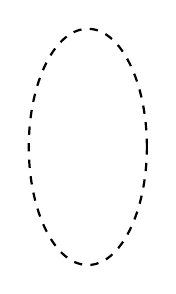
\begin{tikzpicture}
    \draw[thick, dashed] (0,0) ellipse (0.75 and 1.5);
  \end{tikzpicture}
  \end{center}

  \item \textbf{Escrever 3 palavras que começam com O'':}
  \begin{center}
  1. \underline{\hspace{3cm}} \quad 2. \underline{\hspace{3cm}} \quad 3. \underline{\hspace{3cm}}
  \end{center}
\end{enumerate}

\subsection*{PARTE 3: INTEGRAÇÃO (5 itens)}

\begin{enumerate}[resume]
  \item \textbf{Ler em voz alta as palavras abaixo:}
  \begin{center}
  $\rightarrow$ OVO  ~  ONCA  ~  OLHO  ~  OMBRO  ~  ORELHA
  \end{center}

  \item \textbf{Ligar a palavra à figura correspondente:}
  \begin{center}
  \begin{tabular}{cc}
  OVO & \quad --- \quad $\square$ \\
  OLHO & \quad --- \quad $\square$ \\
  ONÇA & \quad --- \quad $\square$
  \end{tabular}
  \end{center}

  \item \textbf{Ler a frase e desenhar o que ela diz:}
  \begin{center}
  $\rightarrow$ O ovo é redondo.
  \end{center}
  \begin{center}
  \begin{tikzpicture}
    \draw[thick, dashed] (0,0) rectangle (6,3);
  \end{tikzpicture}
  \end{center}

  \item \textbf{Completar a frase com O'':}
  \begin{center}
  A m\underline{~~~}la \quad O t\underline{~~~}lho \quad A s\underline{~~~}la
  \end{center}

  \item \textbf{Escrever uma frase usando pelo menos uma palavra com O'':}
  \begin{center}
  \underline{\hspace{12cm}} \\
  \underline{\hspace{12cm}}
  \end{center}
\end{enumerate}

\noindent\textbf{NOTA:} \underline{\hspace{1cm}}/15 \quad $\checkmark$ = 12--15 \quad $\triangle$ = 8--11 \quad $\times$ = menos de 8
\end{exercicio}

\begin{somletra}[title={\faMusic~Atividade de Som da Vogal --- B\^onus (n\~ao vale nota)}]
\textbf{1. Ca\c{c}a ao som.} Marque as palavras que t\^e{}m o som de O:
\begin{center}
$\square$~OVO \quad $\square$~P\'E \quad $\square$~OSSO \quad $\square$~DEDO \quad $\square$~BOLA \quad $\square$~LUA
\end{center}

\textbf{2. Tem ou n\~ao{} tem?} Rodeie SIM ou N\~ao:
\begin{center}
OVO --- (\textbf{SIM}) (\textbf{N\~AO}) \quad P\'E --- (\textbf{SIM}) (\textbf{N\~AO}) \\ OSSO --- (\textbf{SIM}) (\textbf{N\~AO}) \quad DEDO --- (\textbf{SIM}) (\textbf{N\~AO})
\end{center}
\caixapausa{A boca faz bico para o som de O.}
\caixapista{A vogal O aparece na s\'ilaba forte e na fraca.}
\end{somletra}

% bonus_R205_A-04

% FOLHA A-05: LETRA U

\plancheta{Folha A-05 --- Letra U}
\subsection{Folha A-05 --- Letra U}

\begin{exercicio}[Folha de Prática A-05 --- Letra U]
\metadata{A-05}{Pré-silábico}{EF01LP01}{D1}{EF01LP01}{CNE/CEB nº 2/2012}
\kumontiming{1}{90}

\noindent\textbf{Nome:} \underline{\hspace{4cm}} \quad \textbf{Nota:} \underline{\hspace{1cm}}/15

\subsection*{PARTE 1: RECONHECIMENTO (5 itens)}

\begin{enumerate}
  \item \textbf{Circular a letra U'' em meio a outras letras:}
  \begin{center}
  T \quad \textbf{U} \quad V \quad W \quad \textbf{U} \quad X \quad Y \quad \textbf{U} \quad Z \quad A
  \end{center}

  \item \textbf{Sublinhar todas as palavras que começam com U'':}
  \begin{center}
  \uline{uva} \quad bola \quad \uline{unha} \quad sapo \quad \uline{urso} \quad gato \quad \uline{utilidade}
  \end{center}

  \item \textbf{Identificar a letra U'' nas palavras abaixo:}
  \begin{center}
  uva $\rightarrow$ U está na posição \underline{\hspace{1cm}} \\
  unha $\rightarrow$ U está na posição \underline{\hspace{1cm}} \\
  urso $\rightarrow$ U está na posição \underline{\hspace{1cm}}
  \end{center}

  \item \textbf{Dizer em voz alta cada letra e apontar para a U'':}
  \begin{center}
  S \quad T \quad \textbf{U} \quad V \quad W \quad \textbf{U} \quad X \quad Y \quad \textbf{U} \quad Z
  \end{center}

  \item \textbf{Contar quantas vezes a letra U'' aparece:}
  \begin{center}
  UVA $\rightarrow$ quantas U''? \underline{\hspace{1cm}} \\
  UNHA $\rightarrow$ quantas U''? \underline{\hspace{1cm}} \\
  URSO $\rightarrow$ quantas U''? \underline{\hspace{1cm}}
  \end{center}
\end{enumerate}

\subsection*{PARTE 2: PRODUÇÃO GUIADA (5 itens)}

\begin{enumerate}[resume]
  \item \textbf{Copiar a letra U'' cinco vezes:}
  \begin{center}
  U \quad \underline{\hspace{1.5cm}} \quad \underline{\hspace{1.5cm}} \quad \underline{\hspace{1.5cm}} \quad \underline{\hspace{1.5cm}} \quad \underline{\hspace{1.5cm}}
  \end{center}

  \item \textbf{Completar as palavras com a letra U'':}
  \begin{center}
  \underline{U}va \quad \underline{U}nha \quad \underline{U}rso \quad \underline{U}til \quad \underline{U}midade
  \end{center}

  \item \textbf{Escrever a letra U'' maiúscula e minúscula:}
  \begin{center}
  Maiúscula: \underline{\hspace{2cm}} \quad Minúscula: \underline{\hspace{2cm}}
  \end{center}

  \item \textbf{Traçar a letra U'' e copiar:}
  \begin{center}
  \begin{tikzpicture}
    \draw[thick, dashed] (0,3) -- (0,1);
    \draw[thick, dashed] (0,1) .. controls (0.5,0) and (1.5,0) .. (2,1);
    \draw[thick, dashed] (2,1) -- (2,3);
  \end{tikzpicture}
  \end{center}

  \item \textbf{Escrever 3 palavras que começam com U'':}
  \begin{center}
  1. \underline{\hspace{3cm}} \quad 2. \underline{\hspace{3cm}} \quad 3. \underline{\hspace{3cm}}
  \end{center}
\end{enumerate}

\subsection*{PARTE 3: INTEGRAÇÃO (5 itens)}

\begin{enumerate}[resume]
  \item \textbf{Ler em voz alta as palavras abaixo:}
  \begin{center}
  $\rightarrow$ UVA  ~  UNHA  ~  URSO  ~  ÚTIL  ~  UMIDADE
  \end{center}

  \item \textbf{Ligar a palavra à figura correspondente:}
  \begin{center}
  \begin{tabular}{cc}
  UVA & \quad --- \quad $\square$ \\
  URSO & \quad --- \quad $\square$ \\
  UNHA & \quad --- \quad $\square$
  \end{tabular}
  \end{center}

  \item \textbf{Ler a frase e desenhar o que ela diz:}
  \begin{center}
  $\rightarrow$ A uva é roxa.
  \end{center}
  \begin{center}
  \begin{tikzpicture}
    \draw[thick, dashed] (0,0) rectangle (6,3);
  \end{tikzpicture}
  \end{center}

  \item \textbf{Completar a frase com U'':}
  \begin{center}
  A m\underline{~~~}la \quad O t\underline{~~~}lho \quad A s\underline{~~~}la
  \end{center}

  \item \textbf{Escrever uma frase usando pelo menos uma palavra com U'':}
  \begin{center}
  \underline{\hspace{12cm}} \\
  \underline{\hspace{12cm}}
  \end{center}
\end{enumerate}

\noindent\textbf{NOTA:} \underline{\hspace{1cm}}/15 \quad $\checkmark$ = 12--15 \quad $\triangle$ = 8--11 \quad $\times$ = menos de 8
\end{exercicio}

\begin{somletra}[title={\faMusic~Atividade de Som da Vogal --- B\^onus (n\~ao vale nota)}]
\textbf{1. Ca\c{c}a ao som.} Marque as palavras que t\^e{}m o som de U:
\begin{center}
$\square$~UVA \quad $\square$~P\'E \quad $\square$~URSO \quad $\square$~MA\c{c}\~A \quad $\square$~MUNDO \quad $\square$~DEDO
\end{center}

\textbf{2. Tem ou n\~ao{} tem?} Rodeie SIM ou N\~ao:
\begin{center}
UVA --- (\textbf{SIM}) (\textbf{N\~AO}) \quad P\'E --- (\textbf{SIM}) (\textbf{N\~AO}) \\ URSO --- (\textbf{SIM}) (\textbf{N\~AO}) \quad MA\c{c}\~A --- (\textbf{SIM}) (\textbf{N\~AO})
\end{center}
\caixapausa{A boca faz bico pequeno para o som de U.}
\caixapista{A vogal U aparece na s\'ilaba forte e na fraca.}
\end{somletra}

% bonus_R205_A-05

%% ============================================================
%% SEÇÃO 2: REVISÃO DE VOGAIS
%% ============================================================

\section{Folha de Revisão --- Vogais (Pré-silábico/Silábico)}

% FOLHA R-01: REVISÃO VOGAIS

\plancheta{Folha R-01 --- Revisão Vogais}
\subsection{Folha R-01 --- Revisão Vogais}

\begin{exercicio}[Folha de Prática R-01 --- Revisão Vogais]
\metadata{R-01}{Pré-silábico/Silábico}{EF01LP01, EF01LP03}{D1, D5}{EF01LP01}{CNE/CEB nº 2/2012}
\kumontiming{2}{90}

\noindent\textbf{Nome:} \underline{\hspace{4cm}} \quad \textbf{Nota:} \underline{\hspace{1cm}}/15

\subsection*{PARTE 1: RECONHECIMENTO (5 itens)}

\begin{enumerate}
  \item \textbf{Escrever cada vogal maiúscula e minúscula:}
  \begin{center}
  A/a: \underline{\hspace{1.5cm}} \quad E/e: \underline{\hspace{1.5cm}} \quad I/i: \underline{\hspace{1.5cm}} \quad O/o: \underline{\hspace{1.5cm}} \quad U/u: \underline{\hspace{1.5cm}}
  \end{center}

  \item \textbf{Identificar a vogal que falta em cada palavra:}
  \begin{center}
  \underline{A}vão \quad m\underline{E}sa \quad s\underline{I}po \quad c\underline{O}sa \quad l\underline{U}vro
  \end{center}

  \item \textbf{Circular a vogal que está em destaque (negrito):}
  \begin{center}
  \textbf{A}gua \quad el\textbf{E}fante \quad \textbf{I}greja \quad ov\textbf{O} \quad \textbf{U}va
  \end{center}

  \item \textbf{Separar palavras em sílabas e identificar as vogais:}
  \begin{center}
  A-GUA $\rightarrow$ vogais: \underline{\hspace{2cm}} \\
  E-LE-FAN-TE $\rightarrow$ vogais: \underline{\hspace{2cm}} \\
  I-GRE-JA $\rightarrow$ vogais: \underline{\hspace{2cm}}
  \end{center}

  \item \textbf{Classificar as palavras pelo número de sílabas:}
  \begin{center}
  \begin{tabular}{|c|c|c|}
  \hline
  1 sílaba & 2 sílabas & 3 sílabas ou mais \\
  \hline
  \underline{\hspace{3cm}} & \underline{\hspace{3cm}} & \underline{\hspace{3cm}} \\
  \hline
  \end{tabular}
  \end{center}
  Palavras: OVO, ÁGUA, ELEFANTE, UVA, ESCOLA, IGREJA
\end{enumerate}

\subsection*{PARTE 2: PRODUÇÃO GUIADA (5 itens)}

\begin{enumerate}[resume]
  \item \textbf{Escrever 2 palavras que começam com cada vogal:}
  \begin{center}
  \begin{tabular}{ll}
  A: \underline{\hspace{3cm}} \underline{\hspace{3cm}} &
  E: \underline{\hspace{3cm}} \underline{\hspace{3cm}} \\[0.5em]
  I: \underline{\hspace{3cm}} \underline{\hspace{3cm}} &
  O: \underline{\hspace{3cm}} \underline{\hspace{3cm}} \\[0.5em]
  U: \underline{\hspace{3cm}} \underline{\hspace{3cm}} &
  \end{tabular}
  \end{center}

  \item \textbf{Completar as palavras com a vogal correta:}
  \begin{center}
  B\underline{~~~}la \quad S\underline{~~~}po \quad M\underline{~~~}la \quad L\underline{~~~}vro \quad T\underline{~~~}la
  \end{center}

  \item \textbf{Escrever a vogal que ouve:}
  \begin{center}
  Professor diz: ÁGUA'' $\rightarrow$ \underline{\hspace{1cm}} \\
  Professor diz: ELEFANTE'' $\rightarrow$ \underline{\hspace{1cm}} \\
  Professor diz: IGREJA'' $\rightarrow$ \underline{\hspace{1cm}}
  \end{center}

  \item \textbf{Copiar corretamente as palavras abaixo:}
  \begin{center}
  água \quad \underline{\hspace{3cm}} \\
  escola \quad \underline{\hspace{3cm}} \\
  igreja \quad \underline{\hspace{3cm}}
  \end{center}

  \item \textbf{Escrever cada vogal 3 vezes em coluna:}
  \begin{center}
  \begin{tabular}{ccccc}
  A & E & I & O & U \\
  \underline{\hspace{1cm}} & \underline{\hspace{1cm}} & \underline{\hspace{1cm}} & \underline{\hspace{1cm}} & \underline{\hspace{1cm}} \\
  \underline{\hspace{1cm}} & \underline{\hspace{1cm}} & \underline{\hspace{1cm}} & \underline{\hspace{1cm}} & \underline{\hspace{1cm}} \\
  \underline{\hspace{1cm}} & \underline{\hspace{1cm}} & \underline{\hspace{1cm}} & \underline{\hspace{1cm}} & \underline{\hspace{1cm}} \\
  \end{tabular}
  \end{center}
\end{enumerate}

\subsection*{PARTE 3: INTEGRAÇÃO (5 itens)}

\begin{enumerate}[resume]
  \item \textbf{Ler em voz alta as palavras abaixo:}
  \begin{center}
  $\rightarrow$ ÁGUA  ~  ESCOLA  ~  IGREJA  ~  OVO  ~  UVA  ~  ELEFANTE
  \end{center}

  \item \textbf{Ler as frases e apontar para a palavra com a vogal indicada:}
  \begin{center}
  A água é azul.'' $\rightarrow$ palavra com A'': \underline{\hspace{3cm}} \\
  O elefante é grande.'' $\rightarrow$ palavra com E'': \underline{\hspace{3cm}} \\
  A igreja é bonita.'' $\rightarrow$ palavra com I'': \underline{\hspace{3cm}}
  \end{center}

  \item \textbf{Ler e desenhar:}
  \begin{center}
  $\rightarrow$ O ovo está na mesa.
  \end{center}
  \begin{center}
  \begin{tikzpicture}
    \draw[thick, dashed] (0,0) rectangle (6,3);
  \end{tikzpicture}
  \end{center}

  \item \textbf{Completar as frases com a vogal correta:}
  \begin{center}
  A m\underline{~~~}la \quad O t\underline{~~~}lho \quad A s\underline{~~~}la \quad O g\underline{~~~}to
  \end{center}

  \item \textbf{Escrever uma frase completa usando pelo menos 3 vogais diferentes:}
  \begin{center}
  \underline{\hspace{12cm}} \\
  \underline{\hspace{12cm}}
  \end{center}
\end{enumerate}

\noindent\textbf{NOTA:} \underline{\hspace{1cm}}/15 \quad $\checkmark$ = 12--15 \quad $\triangle$ = 8--11 \quad $\times$ = menos de 8
\end{exercicio}

%% ============================================================
%% SEÇÃO 3: CONSONANTES — SILÁBICO
%% ============================================================

\section{Folhas de Prática --- Consonantes (Silábico)}

% FOLHA B-01: LETRA M

\plancheta{Folha B-01 --- Letra M}
\subsection{Folha B-01 --- Letra M}

\begin{exercicio}[Folha de Prática B-01 --- Letra M]
\metadata{B-01}{Silábico}{EF01LP02}{D1}{EF01LP02}{CNE/CEB nº 2/2012}
\kumontiming{2}{90}

\noindent\textbf{Nome:} \underline{\hspace{4cm}} \quad \textbf{Nota:} \underline{\hspace{1cm}}/15

\subsection*{PARTE 1: RECONHECIMENTO (5 itens)}

\begin{enumerate}
  \item \textbf{Circular todas as letras M'' em meio a outras:}
  \begin{center}
  M \quad A \quad \textbf{M} \quad E \quad I \quad \textbf{M} \quad O \quad U \quad \textbf{M} \quad B
  \end{center}

  \item \textbf{Sublinhar todas as palavras que começam com M'':}
  \begin{center}
  \uline{macaco} \quad gato \quad \uline{mesa} \quad sapo \quad \uline{milho} \quad bola \quad \uline{mão}
  \end{center}

  \item \textbf{Formar sílabas com M e vogais:}
  \begin{center}
  M + A = \underline{\hspace{1.5cm}} \quad M + E = \underline{\hspace{1.5cm}} \quad M + I = \underline{\hspace{1.5cm}} \quad M + O = \underline{\hspace{1.5cm}} \quad M + U = \underline{\hspace{1.5cm}}
  \end{center}

  \item \textbf{Identificar a sílaba MA'' nas palavras abaixo:}
  \begin{center}
  MACACO $\rightarrow$ MA'' está na posição \underline{\hspace{1cm}} \\
  MESA $\rightarrow$ MA'' está na posição \underline{\hspace{1cm}} \\
  MANOEL $\rightarrow$ MA'' está na posição \underline{\hspace{1cm}}
  \end{center}

  \item \textbf{Contar o número de sílabas:}
  \begin{center}
  MACACO $\rightarrow$ \underline{\hspace{1cm}} sílabas \\
  MESA $\rightarrow$ \underline{\hspace{1cm}} sílabas \\
  MILHO $\rightarrow$ \underline{\hspace{1cm}} sílabas
  \end{center}
\end{enumerate}

\subsection*{PARTE 2: PRODUÇÃO GUIADA (5 itens)}

\begin{enumerate}[resume]
  \item \textbf{Copiar as sílabas com M:}
  \begin{center}
  MA \quad \underline{\hspace{1.5cm}} \quad ME \quad \underline{\hspace{1.5cm}} \quad MI \quad \underline{\hspace{1.5cm}} \quad MO \quad \underline{\hspace{1.5cm}} \quad MU \quad \underline{\hspace{1.5cm}}
  \end{center}

  \item \textbf{Completar as palavras com a sílaba MA'':}
  \begin{center}
  \underline{MA}caco \quad \underline{MA}esa \quad \underline{MA}ilho \quad \underline{MA}ão \quad \underline{MA}çã
  \end{center}

  \item \textbf{Separar palavras em sílabas:}
  \begin{center}
  MESA $\rightarrow$ \underline{\hspace{1.5cm}} \quad MACACO $\rightarrow$ \underline{\hspace{1.5cm}} \quad MILHO $\rightarrow$ \underline{\hspace{1.5cm}}
  \end{center}

  \item \textbf{Escrever 3 palavras que começam com M'':}
  \begin{center}
  1. \underline{\hspace{3cm}} \quad 2. \underline{\hspace{3cm}} \quad 3. \underline{\hspace{3cm}}
  \end{center}

  \item \textbf{Formar palavras com as sílabas:}
  \begin{center}
  MA + SA = \underline{\hspace{2cm}} \quad MI + LHO = \underline{\hspace{2cm}} \quad MA + CA = \underline{\hspace{2cm}}
  \end{center}
\end{enumerate}

\subsection*{PARTE 3: INTEGRAÇÃO (5 itens)}

\begin{enumerate}[resume]
  \item \textbf{Ler em voz alta as palavras abaixo:}
  \begin{center}
  $\rightarrow$ MACACO  ~  MESA  ~  MILHO  ~  MÃO  ~  MAÇÃ
  \end{center}

  \item \textbf{Ler as sílabas e depois a palavra completa:}
  \begin{center}
  MA -- SA = \underline{\hspace{2cm}} \quad MI -- LHO = \underline{\hspace{2cm}} \quad MA -- CA -- CO = \underline{\hspace{2cm}}
  \end{center}

  \item \textbf{Ler a frase e desenhar:}
  \begin{center}
  $\rightarrow$ O macaco come milho.
  \end{center}
  \begin{center}
  \begin{tikzpicture}
    \draw[thick, dashed] (0,0) rectangle (6,3);
  \end{tikzpicture}
  \end{center}

  \item \textbf{Completar a frase com M'':}
  \begin{center}
  O \underline{~~~}acaco \quad A \underline{~~~}esa \quad O \underline{~~~}ilho
  \end{center}

  \item \textbf{Escrever uma frase usando palavras com M'':}
  \begin{center}
  \underline{\hspace{12cm}} \\
  \underline{\hspace{12cm}}
  \end{center}
\end{enumerate}

\noindent\textbf{NOTA:} \underline{\hspace{1cm}}/15 \quad $\checkmark$ = 12--15 \quad $\triangle$ = 8--11 \quad $\times$ = menos de 8
\end{exercicio}

\begin{somletra}[title={\faMusic~Atividade de Som da Letra --- B\^onus (n\~ao vale nota)}]
\textbf{1. Ca\c{c}a ao som.} Marque as palavras que t\^e{}m o som de M:
\begin{center}
$\square$~MAM\~AO \quad $\square$~PAPAI \quad $\square$~MENINA \quad $\square$~SAPATO \quad $\square$~CAMA \quad $\square$~DEDO
\end{center}

\textbf{2. Tem ou n\~ao{} tem?} Rodeie SIM ou N\~ao:
\begin{center}
MAM\~AO --- (\textbf{SIM}) (\textbf{N\~AO}) \quad PAPAI --- (\textbf{SIM}) (\textbf{N\~AO}) \\ MENINA --- (\textbf{SIM}) (\textbf{N\~AO}) \quad SAPATO --- (\textbf{SIM}) (\textbf{N\~AO})
\end{center}
\caixapausa{A boca fecha e o som sai pelo nariz.}
\caixapista{A consoante M se junta com a vogal: MA, ME, MI, MO, MU.}
\end{somletra}

% bonus_R205_B-01

% FOLHA B-02: LETRA S

\plancheta{Folha B-02 --- Letra S}
\subsection{Folha B-02 --- Letra S}

\begin{exercicio}[Folha de Prática B-02 --- Letra S]
\metadata{B-02}{Silábico}{EF01LP02}{D1}{EF01LP02}{CNE/CEB nº 2/2012}
\kumontiming{2}{90}

\noindent\textbf{Nome:} \underline{\hspace{4cm}} \quad \textbf{Nota:} \underline{\hspace{1cm}}/15

\subsection*{PARTE 1: RECONHECIMENTO (5 itens)}

\begin{enumerate}
  \item \textbf{Circular todas as letras S'' em meio a outras:}
  \begin{center}
  R \quad S \quad \textbf{S} \quad T \quad U \quad \textbf{S} \quad V \quad W \quad \textbf{S} \quad X
  \end{center}

  \item \textbf{Sublinhar todas as palavras que começam com S'':}
  \begin{center}
  \uline{sapo} \quad bola \quad \uline{sol} \quad gato \quad \uline{sala} \quad mesa \quad \uline{sabão}
  \end{center}

  \item \textbf{Formar sílabas com S e vogais:}
  \begin{center}
  S + A = \underline{\hspace{1.5cm}} \quad S + E = \underline{\hspace{1.5cm}} \quad S + I = \underline{\hspace{1.5cm}} \quad S + O = \underline{\hspace{1.5cm}} \quad S + U = \underline{\hspace{1.5cm}}
  \end{center}

  \item \textbf{Identificar a sílaba SA'' nas palavras abaixo:}
  \begin{center}
  SAPO $\rightarrow$ SA'' está na posição \underline{\hspace{1cm}} \\
  SALA $\rightarrow$ SA'' está na posição \underline{\hspace{1cm}} \\
  SACOLA $\rightarrow$ SA'' está na posição \underline{\hspace{1cm}}
  \end{center}

  \item \textbf{Contar o número de sílabas:}
  \begin{center}
  SAPO $\rightarrow$ \underline{\hspace{1cm}} sílabas \\
  SALA $\rightarrow$ \underline{\hspace{1cm}} sílabas \\
  SACOLA $\rightarrow$ \underline{\hspace{1cm}} sílabas
  \end{center}
\end{enumerate}

\subsection*{PARTE 2: PRODUÇÃO GUIADA (5 itens)}

\begin{enumerate}[resume]
  \item \textbf{Copiar as sílabas com S:}
  \begin{center}
  SA \quad \underline{\hspace{1.5cm}} \quad SE \quad \underline{\hspace{1.5cm}} \quad SI \quad \underline{\hspace{1.5cm}} \quad SO \quad \underline{\hspace{1.5cm}} \quad SU \quad \underline{\hspace{1.5cm}}
  \end{center}

  \item \textbf{Completar as palavras com a sílaba SA'':}
  \begin{center}
  \underline{SA}po \quad \underline{SA}la \quad \underline{SA}co \quad \underline{SA}ol \quad \underline{SA}bão
  \end{center}

  \item \textbf{Separar palavras em sílabas:}
  \begin{center}
  SAPO $\rightarrow$ \underline{\hspace{1.5cm}} \quad SALA $\rightarrow$ \underline{\hspace{1.5cm}} \quad SACOLA $\rightarrow$ \underline{\hspace{1.5cm}}
  \end{center}

  \item \textbf{Escrever 3 palavras que começam com S'':}
  \begin{center}
  1. \underline{\hspace{3cm}} \quad 2. \underline{\hspace{3cm}} \quad 3. \underline{\hspace{3cm}}
  \end{center}

  \item \textbf{Formar palavras com as sílabas:}
  \begin{center}
  SA + LA = \underline{\hspace{2cm}} \quad SO + LA = \underline{\hspace{2cm}} \quad SA + PO = \underline{\hspace{2cm}}
  \end{center}
\end{enumerate}

\subsection*{PARTE 3: INTEGRAÇÃO (5 itens)}

\begin{enumerate}[resume]
  \item \textbf{Ler em voz alta as palavras abaixo:}
  \begin{center}
  $\rightarrow$ SAPO  ~  SALA  ~  SOL  ~  SABÃO  ~  SACOLA
  \end{center}

  \item \textbf{Ler as sílabas e depois a palavra completa:}
  \begin{center}
  SA -- PO = \underline{\hspace{2cm}} \quad SA -- LA = \underline{\hspace{2cm}} \quad SO -- LA = \underline{\hspace{2cm}}
  \end{center}

  \item \textbf{Ler a frase e desenhar:}
  \begin{center}
  $\rightarrow$ O sapo está na sala.
  \end{center}
  \begin{center}
  \begin{tikzpicture}
    \draw[thick, dashed] (0,0) rectangle (6,3);
  \end{tikzpicture}
  \end{center}

  \item \textbf{Completar a frase com S'':}
  \begin{center}
  O \underline{~~~}apo \quad A \underline{~~~}ala \quad O \underline{~~~}ol
  \end{center}

  \item \textbf{Escrever uma frase usando palavras com S'':}
  \begin{center}
  \underline{\hspace{12cm}} \\
  \underline{\hspace{12cm}}
  \end{center}
\end{enumerate}

\noindent\textbf{NOTA:} \underline{\hspace{1cm}}/15 \quad $\checkmark$ = 12--15 \quad $\triangle$ = 8--11 \quad $\times$ = menos de 8
\end{exercicio}

\begin{somletra}[title={\faMusic~Atividade de Som da Letra --- B\^onus (n\~ao vale nota)}]
\textbf{1. Ca\c{c}a ao som.} Marque as palavras que t\^e{}m o som de S:
\begin{center}
$\square$~SAPATO \quad $\square$~BOCA \quad $\square$~SOL \quad $\square$~DADO \quad $\square$~CASA \quad $\square$~M\~AO
\end{center}

\textbf{2. Tem ou n\~ao{} tem?} Rodeie SIM ou N\~ao:
\begin{center}
SAPATO --- (\textbf{SIM}) (\textbf{N\~AO}) \quad BOCA --- (\textbf{SIM}) (\textbf{N\~AO}) \\ SOL --- (\textbf{SIM}) (\textbf{N\~AO}) \quad DADO --- (\textbf{SIM}) (\textbf{N\~AO})
\end{center}
\caixapausa{Os dentes ficam juntos e o ar passa assobiando.}
\caixapista{A consoante S se junta com a vogal: SA, SE, SI, SO, SU.}
\end{somletra}

% bonus_R205_B-02

% FOLHA B-03: LETRA T

\plancheta{Folha B-03 --- Letra T}
\subsection{Folha B-03 --- Letra T}

\begin{exercicio}[Folha de Prática B-03 --- Letra T]
\metadata{B-03}{Silábico}{EF01LP02}{D1}{EF01LP02}{CNE/CEB nº 2/2012}
\kumontiming{2}{90}

\noindent\textbf{Nome:} \underline{\hspace{4cm}} \quad \textbf{Nota:} \underline{\hspace{1cm}}/15

\subsection*{PARTE 1: RECONHECIMENTO (5 itens)}

\begin{enumerate}
  \item \textbf{Circular todas as letras T'' em meio a outras:}
  \begin{center}
  S \quad \textbf{T} \quad U \quad V \quad \textbf{T} \quad W \quad X \quad \textbf{T} \quad Y \quad Z
  \end{center}

  \item \textbf{Sublinhar todas as palavras que começam com T'':}
  \begin{center}
  \uline{tato} \quad bola \quad \uline{telha} \quad sapo \quad \uline{tigre} \quad gato \quad \uline{tubo}
  \end{center}

  \item \textbf{Formar sílabas com T e vogais:}
  \begin{center}
  T + A = \underline{\hspace{1.5cm}} \quad T + E = \underline{\hspace{1.5cm}} \quad T + I = \underline{\hspace{1.5cm}} \quad T + O = \underline{\hspace{1.5cm}} \quad T + U = \underline{\hspace{1.5cm}}
  \end{center}

  \item \textbf{Identificar a sílaba TA'' nas palavras abaixo:}
  \begin{center}
  TATO $\rightarrow$ TA'' está na posição \underline{\hspace{1cm}} \\
  TELHA $\rightarrow$ TA'' está na posição \underline{\hspace{1cm}} \\
  TAMPA $\rightarrow$ TA'' está na posição \underline{\hspace{1cm}}
  \end{center}

  \item \textbf{Contar o número de sílabas:}
  \begin{center}
  TATO $\rightarrow$ \underline{\hspace{1cm}} sílabas \\
  TELHA $\rightarrow$ \underline{\hspace{1cm}} sílabas \\
  TIGRE $\rightarrow$ \underline{\hspace{1cm}} sílabas
  \end{center}
\end{enumerate}

\subsection*{PARTE 2: PRODUÇÃO GUIADA (5 itens)}

\begin{enumerate}[resume]
  \item \textbf{Copiar as sílabas com T:}
  \begin{center}
  TA \quad \underline{\hspace{1.5cm}} \quad TE \quad \underline{\hspace{1.5cm}} \quad TI \quad \underline{\hspace{1.5cm}} \quad TO \quad \underline{\hspace{1.5cm}} \quad TU \quad \underline{\hspace{1.5cm}}
  \end{center}

  \item \textbf{Completar as palavras com a sílaba TA'':}
  \begin{center}
  \underline{TA}to \quad \underline{TA}lha \quad \underline{TA}mpa \quad \underline{TA}bua \quad \underline{TA}rde
  \end{center}

  \item \textbf{Separar palavras em sílabas:}
  \begin{center}
  TATO $\rightarrow$ \underline{\hspace{1.5cm}} \quad TELHA $\rightarrow$ \underline{\hspace{1.5cm}} \quad TIGRE $\rightarrow$ \underline{\hspace{1.5cm}}
  \end{center}

  \item \textbf{Escrever 3 palavras que começam com T'':}
  \begin{center}
  1. \underline{\hspace{3cm}} \quad 2. \underline{\hspace{3cm}} \quad 3. \underline{\hspace{3cm}}
  \end{center}

  \item \textbf{Formar palavras com as sílabas:}
  \begin{center}
  TA + RO = \underline{\hspace{2cm}} \quad TU + RO = \underline{\hspace{2cm}} \quad TE + LA = \underline{\hspace{2cm}}
  \end{center}
\end{enumerate}

\subsection*{PARTE 3: INTEGRAÇÃO (5 itens)}

\begin{enumerate}[resume]
  \item \textbf{Ler em voz alta as palavras abaixo:}
  \begin{center}
  $\rightarrow$ TATO  ~  TELHA  ~  TIGRE  ~  TAMPA  ~  TARDE
  \end{center}

  \item \textbf{Ler as sílabas e depois a palavra completa:}
  \begin{center}
  TA -- TO = \underline{\hspace{2cm}} \quad TE -- LHA = \underline{\hspace{2cm}} \quad TI -- GRE = \underline{\hspace{2cm}}
  \end{center}

  \item \textbf{Ler a frase e desenhar:}
  \begin{center}
  $\rightarrow$ O tigre é forte.
  \end{center}
  \begin{center}
  \begin{tikzpicture}
    \draw[thick, dashed] (0,0) rectangle (6,3);
  \end{tikzpicture}
  \end{center}

  \item \textbf{Completar a frase com T'':}
  \begin{center}
  O \underline{~~~}ato \quad A \underline{~~~}arde \quad O \underline{~~~}igre
  \end{center}

  \item \textbf{Escrever uma frase usando palavras com T'':}
  \begin{center}
  \underline{\hspace{12cm}} \\
  \underline{\hspace{12cm}}
  \end{center}
\end{enumerate}

\noindent\textbf{NOTA:} \underline{\hspace{1cm}}/15 \quad $\checkmark$ = 12--15 \quad $\triangle$ = 8--11 \quad $\times$ = menos de 8
\end{exercicio}

\begin{somletra}[title={\faMusic~Atividade de Som da Letra --- B\^onus (n\~ao vale nota)}]
\textbf{1. Ca\c{c}a ao som.} Marque as palavras que t\^e{}m o som de T:
\begin{center}
$\square$~TATU \quad $\square$~SOL \quad $\square$~TOMATE \quad $\square$~P\~AO \quad $\square$~MATA \quad $\square$~BOCA
\end{center}

\textbf{2. Tem ou n\~ao{} tem?} Rodeie SIM ou N\~ao:
\begin{center}
TATU --- (\textbf{SIM}) (\textbf{N\~AO}) \quad SOL --- (\textbf{SIM}) (\textbf{N\~AO}) \\ TOMATE --- (\textbf{SIM}) (\textbf{N\~AO}) \quad P\~AO --- (\textbf{SIM}) (\textbf{N\~AO})
\end{center}
\caixapausa{A l\'ingua toca os dentes de cima.}
\caixapista{A consoante T se junta com a vogal: TA, TE, TI, TO, TU.}
\end{somletra}

% bonus_R205_B-03

% FOLHA B-04: LETRA R

\plancheta{Folha B-04 --- Letra R}
\subsection{Folha B-04 --- Letra R}

\begin{exercicio}[Folha de Prática B-04 --- Letra R]
\metadata{B-04}{Silábico}{EF01LP02}{D1}{EF01LP02}{CNE/CEB nº 2/2012}
\kumontiming{2}{90}

\noindent\textbf{Nome:} \underline{\hspace{4cm}} \quad \textbf{Nota:} \underline{\hspace{1cm}}/15

\subsection*{PARTE 1: RECONHECIMENTO (5 itens)}

\begin{enumerate}
  \item \textbf{Circular todas as letras R'' em meio a outras:}
  \begin{center}
  Q \quad \textbf{R} \quad S \quad T \quad \textbf{R} \quad U \quad V \quad \textbf{R} \quad W \quad X
  \end{center}

  \item \textbf{Sublinhar todas as palavras que começam com R'':}
  \begin{center}
  \uline{raiz} \quad bola \quad \uline{rosa} \quad sapo \quad \uline{rio} \quad gato \quad \uline{roupa}
  \end{center}

  \item \textbf{Formar sílabas com R e vogais:}
  \begin{center}
  R + A = \underline{\hspace{1.5cm}} \quad R + E = \underline{\hspace{1.5cm}} \quad R + I = \underline{\hspace{1.5cm}} \quad R + O = \underline{\hspace{1.5cm}} \quad R + U = \underline{\hspace{1.5cm}}
  \end{center}

  \item \textbf{Identificar a sílaba RA'' nas palavras abaixo:}
  \begin{center}
  RAIZ $\rightarrow$ RA'' está na posição \underline{\hspace{1cm}} \\
  ROSA $\rightarrow$ RA'' está na posição \underline{\hspace{1cm}} \\
  RAPOSA $\rightarrow$ RA'' está na posição \underline{\hspace{1cm}}
  \end{center}

  \item \textbf{Contar o número de sílabas:}
  \begin{center}
  RAIZ $\rightarrow$ \underline{\hspace{1cm}} sílabas \\
  ROSA $\rightarrow$ \underline{\hspace{1cm}} sílabas \\
  RIO $\rightarrow$ \underline{\hspace{1cm}} sílabas
  \end{center}
\end{enumerate}

\subsection*{PARTE 2: PRODUÇÃO GUIADA (5 itens)}

\begin{enumerate}[resume]
  \item \textbf{Copiar as sílabas com R:}
  \begin{center}
  RA \quad \underline{\hspace{1.5cm}} \quad RE \quad \underline{\hspace{1.5cm}} \quad RI \quad \underline{\hspace{1.5cm}} \quad RO \quad \underline{\hspace{1.5cm}} \quad RU \quad \underline{\hspace{1.5cm}}
  \end{center}

  \item \textbf{Completar as palavras com a sílaba RA'':}
  \begin{center}
  \underline{RA}iz \quad \underline{RA}osa \quad \underline{RA}io \quad \underline{RA}pa \quad \underline{RA}to
  \end{center}

  \item \textbf{Separar palavras em sílabas:}
  \begin{center}
  RAIZ $\rightarrow$ \underline{\hspace{1.5cm}} \quad ROSA $\rightarrow$ \underline{\hspace{1.5cm}} \quad RIO $\rightarrow$ \underline{\hspace{1.5cm}}
  \end{center}

  \item \textbf{Escrever 3 palavras que começam com R'':}
  \begin{center}
  1. \underline{\hspace{3cm}} \quad 2. \underline{\hspace{3cm}} \quad 3. \underline{\hspace{3cm}}
  \end{center}

  \item \textbf{Formar palavras com as sílabas:}
  \begin{center}
  RA + SA = \underline{\hspace{2cm}} \quad RI + O = \underline{\hspace{2cm}} \quad RO + SA = \underline{\hspace{2cm}}
  \end{center}
\end{enumerate}

\subsection*{PARTE 3: INTEGRAÇÃO (5 itens)}

\begin{enumerate}[resume]
  \item \textbf{Ler em voz alta as palavras abaixo:}
  \begin{center}
  $\rightarrow$ RAIZ  ~  ROSA  ~  RIO  ~  ROUPA  ~  RAPOSA
  \end{center}

  \item \textbf{Ler as sílabas e depois a palavra completa:}
  \begin{center}
  RA -- SA = \underline{\hspace{2cm}} \quad RI -- O = \underline{\hspace{2cm}} \quad RO -- SA = \underline{\hspace{2cm}}
  \end{center}

  \item \textbf{Ler a frase e desenhar:}
  \begin{center}
  $\rightarrow$ A rosa é vermelha.
  \end{center}
  \begin{center}
  \begin{tikzpicture}
    \draw[thick, dashed] (0,0) rectangle (6,3);
  \end{tikzpicture}
  \end{center}

  \item \textbf{Completar a frase com R'':}
  \begin{center}
  A \underline{~~~}osa \quad O \underline{~~~}io \quad A \underline{~~~}aposa
  \end{center}

  \item \textbf{Escrever uma frase usando palavras com R'':}
  \begin{center}
  \underline{\hspace{12cm}} \\
  \underline{\hspace{12cm}}
  \end{center}
\end{enumerate}

\noindent\textbf{NOTA:} \underline{\hspace{1cm}}/15 \quad $\checkmark$ = 12--15 \quad $\triangle$ = 8--11 \quad $\times$ = menos de 8
\end{exercicio}

\begin{somletra}[title={\faMusic~Atividade de Som da Letra --- B\^onus (n\~ao vale nota)}]
\textbf{1. Ca\c{c}a ao som.} Marque as palavras que t\^e{}m o som de R:
\begin{center}
$\square$~RATO \quad $\square$~SOL \quad $\square$~ROUPA \quad $\square$~BOCA \quad $\square$~CARRO \quad $\square$~P\'E
\end{center}

\textbf{2. Tem ou n\~ao{} tem?} Rodeie SIM ou N\~ao:
\begin{center}
RATO --- (\textbf{SIM}) (\textbf{N\~AO}) \quad SOL --- (\textbf{SIM}) (\textbf{N\~AO}) \\ ROUPA --- (\textbf{SIM}) (\textbf{N\~AO}) \quad BOCA --- (\textbf{SIM}) (\textbf{N\~AO})
\end{center}
\caixapausa{A l\'ingua vibra no c\'eu da boca.}
\caixapista{O R forte aparece no come\c{c}o e no meio: RA, ROU, CAR.}
\end{somletra}

% bonus_R205_B-04

% FOLHA B-05: LETRA L

\plancheta{Folha B-05 --- Letra L}
\subsection{Folha B-05 --- Letra L}

\begin{exercicio}[Folha de Prática B-05 --- Letra L]
\metadata{B-05}{Silábico}{EF01LP02}{D1}{EF01LP02}{CNE/CEB nº 2/2012}
\kumontiming{2}{90}

\noindent\textbf{Nome:} \underline{\hspace{4cm}} \quad \textbf{Nota:} \underline{\hspace{1cm}}/15

\subsection*{PARTE 1: RECONHECIMENTO (5 itens)}

\begin{enumerate}
  \item \textbf{Circular todas as letras L'' em meio a outras:}
  \begin{center}
  K \quad \textbf{L} \quad M \quad N \quad \textbf{L} \quad O \quad P \quad \textbf{L} \quad Q \quad R
  \end{center}

  \item \textbf{Sublinhar todas as palavras que começam com L'':}
  \begin{center}
  \uline{lata} \quad bola \quad \uline{leão} \quad sapo \quad \uline{livro} \quad gato \quad \uline{luz}
  \end{center}

  \item \textbf{Formar sílabas com L e vogais:}
  \begin{center}
  L + A = \underline{\hspace{1.5cm}} \quad L + E = \underline{\hspace{1.5cm}} \quad L + I = \underline{\hspace{1.5cm}} \quad L + O = \underline{\hspace{1.5cm}} \quad L + U = \underline{\hspace{1.5cm}}
  \end{center}

  \item \textbf{Identificar a sílaba LA'' nas palavras abaixo:}
  \begin{center}
  LATA $\rightarrow$ LA'' está na posição \underline{\hspace{1cm}} \\
  LAPA $\rightarrow$ LA'' está na posição \underline{\hspace{1cm}} \\
  LAPIS $\rightarrow$ LA'' está na posição \underline{\hspace{1cm}}
  \end{center}

  \item \textbf{Contar o número de sílabas:}
  \begin{center}
  LATA $\rightarrow$ \underline{\hspace{1cm}} sílabas \\
  LEÃO $\rightarrow$ \underline{\hspace{1cm}} sílabas \\
  LIVRO $\rightarrow$ \underline{\hspace{1cm}} sílabas
  \end{center}
\end{enumerate}

\subsection*{PARTE 2: PRODUÇÃO GUIADA (5 itens)}

\begin{enumerate}[resume]
  \item \textbf{Copiar as sílabas com L:}
  \begin{center}
  LA \quad \underline{\hspace{1.5cm}} \quad LE \quad \underline{\hspace{1.5cm}} \quad LI \quad \underline{\hspace{1.5cm}} \quad LO \quad \underline{\hspace{1.5cm}} \quad LU \quad \underline{\hspace{1.5cm}}
  \end{center}

  \item \textbf{Completar as palavras com a sílaba LA'':}
  \begin{center}
  \underline{LA}ta \quad \underline{LA}va \quad \underline{LA}pis \quad \underline{LA}rva \quad \underline{LA}mpada
  \end{center}

  \item \textbf{Separar palavras em sílabas:}
  \begin{center}
  LATA $\rightarrow$ \underline{\hspace{1.5cm}} \quad LEÃO $\rightarrow$ \underline{\hspace{1.5cm}} \quad LIVRO $\rightarrow$ \underline{\hspace{1.5cm}}
  \end{center}

  \item \textbf{Escrever 3 palavras que começam com L'':}
  \begin{center}
  1. \underline{\hspace{3cm}} \quad 2. \underline{\hspace{3cm}} \quad 3. \underline{\hspace{3cm}}
  \end{center}

  \item \textbf{Formar palavras com as sílabas:}
  \begin{center}
  LA + TA = \underline{\hspace{2cm}} \quad LI + VRO = \underline{\hspace{2cm}} \quad LE + ãO = \underline{\hspace{2cm}}
  \end{center}
\end{enumerate}

\subsection*{PARTE 3: INTEGRAÇÃO (5 itens)}

\begin{enumerate}[resume]
  \item \textbf{Ler em voz alta as palavras abaixo:}
  \begin{center}
  $\rightarrow$ LATA  ~  LEÃO  ~  LIVRO  ~  LUZ  ~  LÂMPADA
  \end{center}

  \item \textbf{Ler as sílabas e depois a palavra completa:}
  \begin{center}
  LA -- TA = \underline{\hspace{2cm}} \quad LI -- VRO = \underline{\hspace{2cm}} \quad LE -- ãO = \underline{\hspace{2cm}}
  \end{center}

  \item \textbf{Ler a frase e desenhar:}
  \begin{center}
  $\rightarrow$ O leão é forte.
  \end{center}
  \begin{center}
  \begin{tikzpicture}
    \draw[thick, dashed] (0,0) rectangle (6,3);
  \end{tikzpicture}
  \end{center}

  \item \textbf{Completar a frase com L'':}
  \begin{center}
  A \underline{~~~}ata \quad O \underline{~~~}eão \quad O \underline{~~~}ivro
  \end{center}

  \item \textbf{Escrever uma frase usando palavras com L'':}
  \begin{center}
  \underline{\hspace{12cm}} \\
  \underline{\hspace{12cm}}
  \end{center}
\end{enumerate}

\noindent\textbf{NOTA:} \underline{\hspace{1cm}}/15 \quad $\checkmark$ = 12--15 \quad $\triangle$ = 8--11 \quad $\times$ = menos de 8
\end{exercicio}

\begin{somletra}[title={\faMusic~Atividade de Som da Letra --- B\^onus (n\~ao vale nota)}]
\textbf{1. Ca\c{c}a ao som.} Marque as palavras que t\^e{}m o som de L:
\begin{center}
$\square$~LUA \quad $\square$~P\'E \quad $\square$~LEITE \quad $\square$~RATO \quad $\square$~BOLA \quad $\square$~M\~AO
\end{center}

\textbf{2. Tem ou n\~ao{} tem?} Rodeie SIM ou N\~ao:
\begin{center}
LUA --- (\textbf{SIM}) (\textbf{N\~AO}) \quad P\'E --- (\textbf{SIM}) (\textbf{N\~AO}) \\ LEITE --- (\textbf{SIM}) (\textbf{N\~AO}) \quad RATO --- (\textbf{SIM}) (\textbf{N\~AO})
\end{center}
\caixapausa{A l\'ingua toca o c\'eu da boca.}
\caixapista{A consoante L se junta com a vogal: LA, LE, LI, LO, LU.}
\end{somletra}

% bonus_R205_B-05

%% ============================================================
%% SEÇÃO 4: REVISÃO DE CONSONANTES
%% ============================================================

\section{Folha de Revisão --- Consonantes (Silábico)}

% FOLHA R-02: REVISÃO CONSONANTES

\plancheta{Folha R-02 --- Revisão Consonantes}
\subsection{Folha R-02 --- Revisão Consonantes}

\begin{exercicio}[Folha de Prática R-02 --- Revisão Consonantes]
\metadata{R-02}{Silábico}{EF01LP02, EF01LP03}{D1, D5}{EF01LP02}{CNE/CEB nº 2/2012}
\kumontiming{2}{90}

\noindent\textbf{Nome:} \underline{\hspace{4cm}} \quad \textbf{Nota:} \underline{\hspace{1cm}}/15

\subsection*{PARTE 1: RECONHECIMENTO (5 itens)}

\begin{enumerate}
  \item \textbf{Formar todas as sílabas com M, S, T, R, L:}
  \begin{center}
  \begin{tabular}{ccccc}
  MA & SA & TA & RA & LA \\
  ME & SE & TE & RE & LE \\
  MI & SI & TI & RI & LI \\
  MO & SO & TO & RO & LO \\
  MU & SU & TU & RU & LU
  \end{tabular}
  \end{center}

  \item \textbf{Identificar a consonante inicial de cada palavra:}
  \begin{center}
  MESA $\rightarrow$ \underline{\hspace{1cm}} \quad SALA $\rightarrow$ \underline{\hspace{1cm}} \quad TAMPA $\rightarrow$ \underline{\hspace{1cm}} \\
  ROÇA $\rightarrow$ \underline{\hspace{1cm}} \quad LATA $\rightarrow$ \underline{\hspace{1cm}} \quad MONO $\rightarrow$ \underline{\hspace{1cm}}
  \end{center}

  \item \textbf{Separar palavras em sílabas:}
  \begin{center}
  MESA $\rightarrow$ \underline{\hspace{1.5cm}} \quad SALA $\rightarrow$ \underline{\hspace{1.5cm}} \quad TAMPA $\rightarrow$ \underline{\hspace{1.5cm}} \\
  ROÇA $\rightarrow$ \underline{\hspace{1.5cm}} \quad LATA $\rightarrow$ \underline{\hspace{1.5cm}} \quad MOLA $\rightarrow$ \underline{\hspace{1.5cm}}
  \end{center}

  \item \textbf{Classificar palavras pela consoante inicial:}
  \begin{center}
  \begin{tabular}{|c|c|c|c|c|}
  \hline
  M & S & T & R & L \\
  \hline
  \underline{\hspace{2cm}} & \underline{\hspace{2cm}} & \underline{\hspace{2cm}} & \underline{\hspace{2cm}} & \underline{\hspace{2cm}} \\
  \hline
  \end{tabular}
  \end{center}
  Palavras: MESA, SALA, TAMPA, ROÇA, LATA, MILHO, SOL, TIGRE, RIO, LUA

  \item \textbf{Ler as sílabas em sequência:}
  \begin{center}
  MA -- ME -- MI -- MO -- MU \\
  SA -- SE -- SI -- SO -- SU \\
  TA -- TE -- TI -- TO -- TU
  \end{center}
\end{enumerate}

\subsection*{PARTE 2: PRODUÇÃO GUIADA (5 itens)}

\begin{enumerate}[resume]
  \item \textbf{Escrever sílabas com cada consoante:}
  \begin{center}
  \begin{tabular}{ccccc}
  MA & SA & TA & RA & LA \\
  \underline{\hspace{1cm}} & \underline{\hspace{1cm}} & \underline{\hspace{1cm}} & \underline{\hspace{1cm}} & \underline{\hspace{1cm}} \\
  \underline{\hspace{1cm}} & \underline{\hspace{1cm}} & \underline{\hspace{1cm}} & \underline{\hspace{1cm}} & \underline{\hspace{1cm}} \\
  \underline{\hspace{1cm}} & \underline{\hspace{1cm}} & \underline{\hspace{1cm}} & \underline{\hspace{1cm}} & \underline{\hspace{1cm}}
  \end{tabular}
  \end{center}

  \item \textbf{Completar palavras com a consoante correta:}
  \begin{center}
  \underline{M}esa \quad \underline{S}ala \quad \underline{T}ampa \quad \underline{R}oça \quad \underline{L}ata
  \end{center}

  \item \textbf{Formar palavras com as sílabas:}
  \begin{center}
  MA + SA = \underline{\hspace{2cm}} \quad SO + LA = \underline{\hspace{2cm}} \quad TA + PO = \underline{\hspace{2cm}} \\
  RO + ãO = \underline{\hspace{2cm}} \quad LA + VA = \underline{\hspace{2cm}} \quad MI + LHO = \underline{\hspace{2cm}}
  \end{center}

  \item \textbf{Escrever 2 palavras para cada consoante:}
  \begin{center}
  M: \underline{\hspace{3cm}} \underline{\hspace{3cm}} \quad S: \underline{\hspace{3cm}} \underline{\hspace{3cm}} \quad T: \underline{\hspace{3cm}} \underline{\hspace{3cm}} \\
  R: \underline{\hspace{3cm}} \underline{\hspace{3cm}} \quad L: \underline{\hspace{3cm}} \underline{\hspace{3cm}}
  \end{center}

  \item \textbf{Copiar corretamente as palavras abaixo:}
  \begin{center}
  mesa $\rightarrow$ \underline{\hspace{3cm}} \quad sala $\rightarrow$ \underline{\hspace{3cm}} \quad tampa $\rightarrow$ \underline{\hspace{3cm}} \\
  roça $\rightarrow$ \underline{\hspace{3cm}} \quad lata $\rightarrow$ \underline{\hspace{3cm}}
  \end{center}
\end{enumerate}

\subsection*{PARTE 3: INTEGRAÇÃO (5 itens)}

\begin{enumerate}[resume]
  \item \textbf{Ler em voz alta as palavras abaixo:}
  \begin{center}
  $\rightarrow$ MESA  ~  SALA  ~  TAMPA  ~  ROÇA  ~  LATA  ~  MILHO  ~  SOL
  \end{center}

  \item \textbf{Ler as frases e apontar para a palavra com a consoante indicada:}
  \begin{center}
  A mesa é alta.'' $\rightarrow$ palavra com M'': \underline{\hspace{3cm}} \\
  O sapo é verde.'' $\rightarrow$ palavra com S'': \underline{\hspace{3cm}} \\
  A tampa é azul.'' $\rightarrow$ palavra com T'': \underline{\hspace{3cm}}
  \end{center}

  \item \textbf{Ler e desenhar:}
  \begin{center}
  $\rightarrow$ O tigre está na lata.
  \end{center}
  \begin{center}
  \begin{tikzpicture}
    \draw[thick, dashed] (0,0) rectangle (6,3);
  \end{tikzpicture}
  \end{center}

  \item \textbf{Completar as frases com a consoante correta:}
  \begin{center}
  A \underline{~~~}esa \quad O \underline{~~~}apo \quad A \underline{~~~}ampa \quad O \underline{~~~}oço \quad A \underline{~~~}ata
  \end{center}

  \item \textbf{Escrever uma frase completa usando pelo menos 3 consoantes diferentes:}
  \begin{center}
  \underline{\hspace{12cm}} \\
  \underline{\hspace{12cm}}
  \end{center}
\end{enumerate}

\noindent\textbf{NOTA:} \underline{\hspace{1cm}}/15 \quad $\checkmark$ = 12--15 \quad $\triangle$ = 8--11 \quad $\times$ = menos de 8
\end{exercicio}

%% ============================================================
%% SEÇÃO 5: SÍLABAS — SILÁBICO-ALFABÉTICO
%% ============================================================

\section{Folhas de Prática --- Sílabas (Silábico-Alfabético)}

% FOLHA C-01: SÍLABAS COM A

\plancheta{Folha C-01 --- Sílabas com A}
\subsection{Folha C-01 --- Sílabas com A}

\begin{exercicio}[Folha de Prática C-01 --- Sílabas com A]
\metadata{C-01}{Silábico-Alfabético}{EF01LP03}{D1}{EF01LP03}{CNE/CEB nº 2/2012}
\kumontiming{3}{90}

\noindent\textbf{Nome:} \underline{\hspace{4cm}} \quad \textbf{Nota:} \underline{\hspace{1cm}}/15

\subsection*{PARTE 1: RECONHECIMENTO (5 itens)}

\begin{enumerate}
  \item \textbf{Ler as sílabas com A'' em voz alta:}
  \begin{center}
  MA \quad SA \quad TA \quad RA \quad LA \quad BA \quad CA \quad DA \quad FA \quad GA
  \end{center}

  \item \textbf{Identificar a sílaba que falta na palavra:}
  \begin{center}
  MA -- SA = M\underline{~~~}SA \quad SA -- LA = S\underline{~~~}LA \quad TA -- PA = T\underline{~~~}PA \\
  RO -- SA = R\underline{~~~}SA \quad LA -- TA = L\underline{~~~}TA \quad BA -- LA = B\underline{~~~}LA
  \end{center}

  \item \textbf{Separar palavras em sílabas:}
  \begin{center}
  MACACO $\rightarrow$ \underline{\hspace{1.5cm}} \quad SALA $\rightarrow$ \underline{\hspace{1.5cm}} \quad TAMPA $\rightarrow$ \underline{\hspace{1.5cm}} \\
  RAPSA $\rightarrow$ \underline{\hspace{1.5cm}} \quad LATA $\rightarrow$ \underline{\hspace{1.5cm}} \quad BALA $\rightarrow$ \underline{\hspace{1.5cm}}
  \end{center}

  \item \textbf{Contar o número de sílabas em cada palavra:}
  \begin{center}
  MACACO $\rightarrow$ \underline{\hspace{1cm}} sílabas \\
  SALA $\rightarrow$ \underline{\hspace{1cm}} sílabas \\
  TAMPA $\rightarrow$ \underline{\hspace{1cm}} sílabas \\
  LATA $\rightarrow$ \underline{\hspace{1cm}} sílabas
  \end{center}

  \item \textbf{Ler as sílabas em sequência e formar palavras:}
  \begin{center}
  MA -- SA = \underline{\hspace{2cm}} \quad SA -- LA = \underline{\hspace{2cm}} \quad TA -- PA = \underline{\hspace{2cm}} \\
  RO -- SA = \underline{\hspace{2cm}} \quad LA -- TA = \underline{\hspace{2cm}} \quad BA -- LA = \underline{\hspace{2cm}}
  \end{center}
\end{enumerate}

\subsection*{PARTE 2: PRODUÇÃO GUIADA (5 itens)}

\begin{enumerate}[resume]
  \item \textbf{Escrever sílabas com A'' usando consoantes diferentes:}
  \begin{center}
  \underline{\hspace{1.5cm}}A \quad \underline{\hspace{1.5cm}}A \quad \underline{\hspace{1.5cm}}A \quad \underline{\hspace{1.5cm}}A \quad \underline{\hspace{1.5cm}}A
  \end{center}

  \item \textbf{Completar as palavras com a sílaba correta:}
  \begin{center}
  \underline{MA}caco \quad \underline{SA}la \quad \underline{TA}mpa \quad \underline{RO}ça \quad \underline{LA}ta
  \end{center}

  \item \textbf{Escrever palavras que contenham MA'':}
  \begin{center}
  1. \underline{\hspace{3cm}} \quad 2. \underline{\hspace{3cm}} \quad 3. \underline{\hspace{3cm}}
  \end{center}

  \item \textbf{Escrever palavras que contenham SA'':}
  \begin{center}
  1. \underline{\hspace{3cm}} \quad 2. \underline{\hspace{3cm}} \quad 3. \underline{\hspace{3cm}}
  \end{center}

  \item \textbf{Formar palavras usando as sílabas dadas:}
  \begin{center}
  MA + CA + CO = \underline{\hspace{2cm}} \quad SA + LA = \underline{\hspace{2cm}} \quad TA + PA = \underline{\hspace{2cm}} \\
  RO + SA = \underline{\hspace{2cm}} \quad LA + TA = \underline{\hspace{2cm}} \quad BA + LA = \underline{\hspace{2cm}}
  \end{center}
\end{enumerate}

\subsection*{PARTE 3: INTEGRAÇÃO (5 itens)}

\begin{enumerate}[resume]
  \item \textbf{Ler em voz alta as palavras abaixo:}
  \begin{center}
  $\rightarrow$ MACACO  ~  SALA  ~  TAMPA  ~  ROÇA  ~  LATA  ~  BALA  ~  MESA
  \end{center}

  \item \textbf{Ler as frases e sublinhar todas as palavras com A'':}
  \begin{center}
  A mesa é alta.'' $\rightarrow$ \underline{\hspace{5cm}} \\
  O macaco come banana.'' $\rightarrow$ \underline{\hspace{5cm}}
  \end{center}

  \item \textbf{Ler e desenhar:}
  \begin{center}
  $\rightarrow$ O macaco está na sala.
  \end{center}
  \begin{center}
  \begin{tikzpicture}
    \draw[thick, dashed] (0,0) rectangle (6,3);
  \end{tikzpicture}
  \end{center}

  \item \textbf{Completar as palavras com A'':}
  \begin{center}
  M\underline{~~~}SA \quad S\underline{~~~}LA \quad T\underline{~~~}PA \quad R\underline{~~~}SA \quad L\underline{~~~}TA
  \end{center}

  \item \textbf{Escrever uma frase usando pelo menos 3 palavras com A'':}
  \begin{center}
  \underline{\hspace{12cm}} \\
  \underline{\hspace{12cm}}
  \end{center}
\end{enumerate}

\noindent\textbf{NOTA:} \underline{\hspace{1cm}}/15 \quad $\checkmark$ = 12--15 \quad $\triangle$ = 8--11 \quad $\times$ = menos de 8
\end{exercicio}

\begin{somsilaba}[title={\faMusic~Som das S\'ilabas --- B\^onus (n\~ao vale nota)}]
\textbf{Desafio de consci\^encia sil\'abica:} ou\c{c}a, bata palmas e conte as s\'ilabas:
\begin{center}
MA.CA.CO $\rightarrow$ \underline{\hspace{1cm}} s\'ilabas \quad TAM.PA $\rightarrow$ \underline{\hspace{1cm}} s\'ilabas \quad SA.LA $\rightarrow$ \underline{\hspace{1cm}} s\'ilabas
\end{center}
\caixapista{TAM.PA: a s\'ilaba com som de A \'e TAM.}
\end{somsilaba}

% bônus_C-01 (R204)

% FOLHA C-02: SÍLABAS COM E/I

\plancheta{Folha C-02 --- Sílabas com E/I}
\subsection{Folha C-02 --- Sílabas com E/I}

\begin{exercicio}[Folha de Prática C-02 --- Sílabas com E/I]
\metadata{C-02}{Silábico-Alfabético}{EF01LP03}{D1}{EF01LP03}{CNE/CEB nº 2/2012}
\kumontiming{3}{90}

\noindent\textbf{Nome:} \underline{\hspace{4cm}} \quad \textbf{Nota:} \underline{\hspace{1cm}}/15

\subsection*{PARTE 1: RECONHECIMENTO (5 itens)}

\begin{enumerate}
  \item \textbf{Ler as sílabas com E'' e I'' em voz alta:}
  \begin{center}
  ME \quad SE \quad TE \quad RE \quad LE \quad MI \quad SI \quad TI \quad RI \quad LI
  \end{center}

  \item \textbf{Identificar se a sílaba contém E'' ou I'':}
  \begin{center}
  MESA $\rightarrow$ sílaba com \underline{\hspace{1cm}}'' \quad SILVA $\rightarrow$ sílaba com \underline{\hspace{1cm}}'' \\
  TENIS $\rightarrow$ sílaba com \underline{\hspace{1cm}}'' \quad RISCO $\rightarrow$ sílaba com \underline{\hspace{1cm}}''
  \end{center}

  \item \textbf{Separar palavras em sílabas:}
  \begin{center}
  ELEFANTE $\rightarrow$ \underline{\hspace{1.5cm}} \quad SILVA $\rightarrow$ \underline{\hspace{1.5cm}} \quad TENIS $\rightarrow$ \underline{\hspace{1.5cm}} \\
  RISCO $\rightarrow$ \underline{\hspace{1.5cm}} \quad MESA $\rightarrow$ \underline{\hspace{1.5cm}} \quad LIXO $\rightarrow$ \underline{\hspace{1.5cm}}
  \end{center}

  \item \textbf{Contar o número de sílabas:}
  \begin{center}
  ELEFANTE $\rightarrow$ \underline{\hspace{1cm}} sílabas \\
  SILVA $\rightarrow$ \underline{\hspace{1cm}} sílabas \\
  TENIS $\rightarrow$ \underline{\hspace{1cm}} sílabas \\
  RISCO $\rightarrow$ \underline{\hspace{1cm}} sílabas
  \end{center}

  \item \textbf{Ler as sílabas e formar palavras:}
  \begin{center}
  ME -- SA = \underline{\hspace{2cm}} \quad SI -- LVA = \underline{\hspace{2cm}} \quad TE -- NIS = \underline{\hspace{2cm}} \\
  RI -- SCO = \underline{\hspace{2cm}} \quad LI -- XO = \underline{\hspace{2cm}} \quad ME -- NI -- NO = \underline{\hspace{2cm}}
  \end{center}
\end{enumerate}

\subsection*{PARTE 2: PRODUÇÃO GUIADA (5 itens)}

\begin{enumerate}[resume]
  \item \textbf{Escrever sílabas com E'':}
  \begin{center}
  \underline{\hspace{1.5cm}}E \quad \underline{\hspace{1.5cm}}E \quad \underline{\hspace{1.5cm}}E \quad \underline{\hspace{1.5cm}}E \quad \underline{\hspace{1.5cm}}E
  \end{center}

  \item \textbf{Escrever sílabas com I'':}
  \begin{center}
  \underline{\hspace{1.5cm}}I \quad \underline{\hspace{1.5cm}}I \quad \underline{\hspace{1.5cm}}I \quad \underline{\hspace{1.5cm}}I \quad \underline{\hspace{1.5cm}}I
  \end{center}

  \item \textbf{Completar as palavras com E'' ou I'':}
  \begin{center}
  M\underline{~~~}SA \quad S\underline{~~~}LVA \quad T\underline{~~~}NIS \quad R\underline{~~~}SCO \quad L\underline{~~~}XO
  \end{center}

  \item \textbf{Escrever 3 palavras com E'' e 3 com I'':}
  \begin{center}
  Com E'': \underline{\hspace{2.2cm}} \underline{\hspace{2.2cm}} \underline{\hspace{2.2cm}} \\
  Com I'': \underline{\hspace{2.2cm}} \underline{\hspace{2.2cm}} \underline{\hspace{2.2cm}}
  \end{center}

  \item \textbf{Formar palavras com as sílabas:}
  \begin{center}
  ME + SA = \underline{\hspace{2cm}} \quad SI + LVA = \underline{\hspace{2cm}} \quad TE + NIS = \underline{\hspace{2cm}} \\
  RI + SCO = \underline{\hspace{2cm}} \quad LI + XO = \underline{\hspace{2cm}}
  \end{center}
\end{enumerate}

\subsection*{PARTE 3: INTEGRAÇÃO (5 itens)}

\begin{enumerate}[resume]
  \item \textbf{Ler em voz alta as palavras abaixo:}
  \begin{center}
  $\rightarrow$ MESA  ~  SILVA  ~  TENIS  ~  RISCO  ~  LIXO  ~  ELEFANTE  ~  MENINO
  \end{center}

  \item \textbf{Ler as frases e sublinhar as palavras com E'':}
  \begin{center}
  O elefante é grande.'' $\rightarrow$ \underline{\hspace{5cm}} \\
  O menino tem um tênis.'' $\rightarrow$ \underline{\hspace{5cm}}
  \end{center}

  \item \textbf{Ler e desenhar:}
  \begin{center}
  $\rightarrow$ O elefante está na escola.
  \end{center}
  \begin{center}
  \begin{tikzpicture}
    \draw[thick, dashed] (0,0) rectangle (6,3);
  \end{tikzpicture}
  \end{center}

  \item \textbf{Completar as frases com E'' ou I'':}
  \begin{center}
  A m\underline{~~~}sa \quad O sil\underline{~~~}vo \quad O t\underline{~~~}nis \quad O r\underline{~~~}sco \quad O l\underline{~~~}xo
  \end{center}

  \item \textbf{Escrever uma frase usando palavras com E'' e I'':}
  \begin{center}
  \underline{\hspace{12cm}} \\
  \underline{\hspace{12cm}}
  \end{center}
\end{enumerate}

\noindent\textbf{NOTA:} \underline{\hspace{1cm}}/15 \quad $\checkmark$ = 12--15 \quad $\triangle$ = 8--11 \quad $\times$ = menos de 8
\end{exercicio}

\begin{somsilaba}[title={\faMusic~Som das S\'ilabas --- B\^onus (n\~ao vale nota)}]
\textbf{Desafio de consci\^encia sil\'abica:} ou\c{c}a, bata palmas e conte as s\'ilabas:
\begin{center}
ME.SA $\rightarrow$ \underline{\hspace{1cm}} s\'ilabas \quad CE.DO $\rightarrow$ \underline{\hspace{1cm}} s\'ilabas \quad A.MI.GO $\rightarrow$ \underline{\hspace{1cm}} s\'ilabas
\end{center}
\caixapista{ME.SA: o som de E est\'a em ME.}
\end{somsilaba}

% bônus_C-02 (R204)

% FOLHA C-03: SÍLABAS COM O/U

\plancheta{Folha C-03 --- Sílabas com O/U}
\subsection{Folha C-03 --- Sílabas com O/U}

\begin{exercicio}[Folha de Prática C-03 --- Sílabas com O/U]
\metadata{C-03}{Silábico-Alfabético}{EF01LP03}{D1}{EF01LP03}{CNE/CEB nº 2/2012}
\kumontiming{3}{90}

\noindent\textbf{Nome:} \underline{\hspace{4cm}} \quad \textbf{Nota:} \underline{\hspace{1cm}}/15

\subsection*{PARTE 1: RECONHECIMENTO (5 itens)}

\begin{enumerate}
  \item \textbf{Ler as sílabas com O'' e U'' em voz alta:}
  \begin{center}
  MO \quad SO \quad TO \quad RO \quad LO \quad MU \quad SU \quad TU \quad RU \quad LU
  \end{center}

  \item \textbf{Identificar se a sílaba contém O'' ou U'':}
  \begin{center}
  MOLA $\rightarrow$ sílaba com \underline{\hspace{1cm}}'' \quad SUSTO $\rightarrow$ sílaba com \underline{\hspace{1cm}}'' \\
  TOALHA $\rightarrow$ sílaba com \underline{\hspace{1cm}}'' \quad RUBRO $\rightarrow$ sílaba com \underline{\hspace{1cm}}''
  \end{center}

  \item \textbf{Separar palavras em sílabas:}
  \begin{center}
  MOLA $\rightarrow$ \underline{\hspace{1.5cm}} \quad SUSTO $\rightarrow$ \underline{\hspace{1.5cm}} \quad TOALHA $\rightarrow$ \underline{\hspace{1.5cm}} \\
  RUBRO $\rightarrow$ \underline{\hspace{1.5cm}} \quad LONA $\rightarrow$ \underline{\hspace{1.5cm}} \quad LUA $\rightarrow$ \underline{\hspace{1.5cm}}
  \end{center}

  \item \textbf{Contar o número de sílabas:}
  \begin{center}
  MOLA $\rightarrow$ \underline{\hspace{1cm}} sílabas \\
  SUSTO $\rightarrow$ \underline{\hspace{1cm}} sílabas \\
  TOALHA $\rightarrow$ \underline{\hspace{1cm}} sílabas \\
  LONA $\rightarrow$ \underline{\hspace{1cm}} sílabas
  \end{center}

  \item \textbf{Ler as sílabas e formar palavras:}
  \begin{center}
  MO + LA = \underline{\hspace{2cm}} \quad SU + STO = \underline{\hspace{2cm}} \quad TO + ALHA = \underline{\hspace{2cm}} \\
  RU + BRO = \underline{\hspace{2cm}} \quad LO + NA = \underline{\hspace{2cm}} \quad LU + A = \underline{\hspace{2cm}}
  \end{center}
\end{enumerate}

\subsection*{PARTE 2: PRODUÇÃO GUIADA (5 itens)}

\begin{enumerate}[resume]
  \item \textbf{Escrever sílabas com O'':}
  \begin{center}
  \underline{\hspace{1.5cm}}O \quad \underline{\hspace{1.5cm}}O \quad \underline{\hspace{1.5cm}}O \quad \underline{\hspace{1.5cm}}O \quad \underline{\hspace{1.5cm}}O
  \end{center}

  \item \textbf{Escrever sílabas com U'':}
  \begin{center}
  \underline{\hspace{1.5cm}}U \quad \underline{\hspace{1.5cm}}U \quad \underline{\hspace{1.5cm}}U \quad \underline{\hspace{1.5cm}}U \quad \underline{\hspace{1.5cm}}U
  \end{center}

  \item \textbf{Completar as palavras com O'' ou U'':}
  \begin{center}
  M\underline{~~~}LA \quad S\underline{~~~}STO \quad T\underline{~~~}ALHA \quad R\underline{~~~}BRO \quad L\underline{~~~}NA
  \end{center}

  \item \textbf{Escrever 3 palavras com O'' e 3 com U'':}
  \begin{center}
  Com O'': \underline{\hspace{2.2cm}} \underline{\hspace{2.2cm}} \underline{\hspace{2.2cm}} \\
  Com U'': \underline{\hspace{2.2cm}} \underline{\hspace{2.2cm}} \underline{\hspace{2.2cm}}
  \end{center}

  \item \textbf{Formar palavras com as sílabas:}
  \begin{center}
  MO + LA = \underline{\hspace{2cm}} \quad SU + STO = \underline{\hspace{2cm}} \quad TO + ALHA = \underline{\hspace{2cm}} \\
  RU + BRO = \underline{\hspace{2cm}} \quad LO + NA = \underline{\hspace{2cm}} \quad LU + A = \underline{\hspace{2cm}}
  \end{center}
\end{enumerate}

\subsection*{PARTE 3: INTEGRAÇÃO (5 itens)}

\begin{enumerate}[resume]
  \item \textbf{Ler em voz alta as palavras abaixo:}
  \begin{center}
  $\rightarrow$ MOLA  ~  SUSTO  ~  TOALHA  ~  RUBRO  ~  LONA  ~  LUA  ~  MONO
  \end{center}

  \item \textbf{Ler as frases e sublinhar as palavras com O'':}
  \begin{center}
  A lua é bonita.'' $\rightarrow$ \underline{\hspace{5cm}} \\
  O homem tem susto.'' $\rightarrow$ \underline{\hspace{5cm}}
  \end{center}

  \item \textbf{Ler e desenhar:}
  \begin{center}
  $\rightarrow$ A lua está no céu.
  \end{center}
  \begin{center}
  \begin{tikzpicture}
    \draw[thick, dashed] (0,0) rectangle (6,3);
  \end{tikzpicture}
  \end{center}

  \item \textbf{Completar as frases com O'' ou U'':}
  \begin{center}
  A m\underline{~~~}la \quad O s\underline{~~~}sto \quad A t\underline{~~~}alha \quad O r\underline{~~~}bro \quad A l\underline{~~~}na
  \end{center}

  \item \textbf{Escrever uma frase usando palavras com O'' e U'':}
  \begin{center}
  \underline{\hspace{12cm}} \\
  \underline{\hspace{12cm}}
  \end{center}
\end{enumerate}

\noindent\textbf{NOTA:} \underline{\hspace{1cm}}/15 \quad $\checkmark$ = 12--15 \quad $\triangle$ = 8--11 \quad $\times$ = menos de 8
\end{exercicio}

\begin{somsilaba}[title={\faMusic~Som das S\'ilabas --- B\^onus (n\~ao vale nota)}]
\textbf{Desafio de consci\^encia sil\'abica:} ou\c{c}a, bata palmas e conte as s\'ilabas:
\begin{center}
BO.LA $\rightarrow$ \underline{\hspace{1cm}} s\'ilabas \quad UR.SO $\rightarrow$ \underline{\hspace{1cm}} s\'ilabas \quad FO.GO $\rightarrow$ \underline{\hspace{1cm}} s\'ilabas
\end{center}
\caixapista{UR.SO: o som de U est\'a em UR.}
\end{somsilaba}

% bônus_C-03 (R204)

%% ============================================================
%% SEÇÃO 6: REVISÃO DE SÍLABAS
%% ============================================================

\section{Folha de Revisão --- Sílabas (Silábico-Alfabético)}

% FOLHA R-03: REVISÃO SÍLABAS

\plancheta{Folha R-03 --- Revisão Sílabas}
\subsection{Folha R-03 --- Revisão Sílabas}

\begin{exercicio}[Folha de Prática R-03 --- Revisão Sílabas]
\metadata{R-03}{Silábico-Alfabético}{EF01LP03, EF01LP04}{D1, D5}{EF01LP03}{CNE/CEB nº 2/2012}
\kumontiming{3}{90}

\noindent\textbf{Nome:} \underline{\hspace{4cm}} \quad \textbf{Nota:} \underline{\hspace{1cm}}/15

\subsection*{PARTE 1: RECONHECIMENTO (5 itens)}

\begin{enumerate}
  \item \textbf{Ler todas as sílabas com todas as consoantes e vogais:}
  \begin{center}
  \begin{tabular}{ccccc}
  MA & SA & TA & RA & LA \\
  ME & SE & TE & RE & LE \\
  MI & SI & TI & RI & LI \\
  MO & SO & TO & RO & LO \\
  MU & SU & TU & RU & LU
  \end{tabular}
  \end{center}

  \item \textbf{Separar palavras em sílabas:}
  \begin{center}
  MACACO $\rightarrow$ \underline{\hspace{1.5cm}} \quad MESA $\rightarrow$ \underline{\hspace{1.5cm}} \quad SALA $\rightarrow$ \underline{\hspace{1.5cm}} \\
  TAMPA $\rightarrow$ \underline{\hspace{1.5cm}} \quad ROÇA $\rightarrow$ \underline{\hspace{1.5cm}} \quad LATA $\rightarrow$ \underline{\hspace{1.5cm}} \\
  MOLA $\rightarrow$ \underline{\hspace{1.5cm}} \quad SUSTO $\rightarrow$ \underline{\hspace{1.5cm}} \quad TOALHA $\rightarrow$ \underline{\hspace{1.5cm}}
  \end{center}

  \item \textbf{Identificar a sílaba que falta:}
  \begin{center}
  MA -- SA = \underline{\hspace{1cm}}SA \quad SA -- LA = S\underline{\hspace{1cm}}LA \quad TA -- PA = T\underline{\hspace{1cm}}PA \\
  RO -- SA = R\underline{\hspace{1cm}}SA \quad LA -- TA = L\underline{\hspace{1cm}}TA \quad MO -- LA = M\underline{\hspace{1cm}}LA
  \end{center}

  \item \textbf{Classificar palavras pelo número de sílabas:}
  \begin{center}
  \begin{tabular}{|c|c|c|}
  \hline
  1 sílaba & 2 sílabas & 3 sílabas ou mais \\
  \hline
  \underline{\hspace{3cm}} & \underline{\hspace{3cm}} & \underline{\hspace{3cm}} \\
  \hline
  \end{tabular}
  \end{center}
  Palavras: SOL, MESA, MACACO, SALA, TAMPA, ROÇA, ELEFANTE, LATA

  \item \textbf{Ler em voz alta as sílabas e palavras:}
  \begin{center}
  MA--SA $\rightarrow$ MESA \quad SA--LA $\rightarrow$ SALA \quad TA--PA $\rightarrow$ TAMPA \\
  RO--SA $\rightarrow$ ROÇA \quad LA--TA $\rightarrow$ LATA \quad MO--LA $\rightarrow$ MOLA
  \end{center}
\end{enumerate}

\subsection*{PARTE 2: PRODUÇÃO GUIADA (5 itens)}

\begin{enumerate}[resume]
  \item \textbf{Escrever sílabas com cada consoante:}
  \begin{center}
  M: \underline{\hspace{3cm}} \quad S: \underline{\hspace{3cm}} \quad T: \underline{\hspace{3cm}} \\
  R: \underline{\hspace{3cm}} \quad L: \underline{\hspace{3cm}}
  \end{center}

  \item \textbf{Completar palavras com a sílaba correta:}
  \begin{center}
  \underline{MA}caco \quad \underline{SA}la \quad \underline{TA}mpa \quad \underline{RO}ça \quad \underline{LA}ta \\
  \underline{MO}la \quad \underline{SU}sto \quad \underline{TO}alha \quad \underline{RU}bro \quad \underline{LO}na
  \end{center}

  \item \textbf{Formar palavras com as sílabas:}
  \begin{center}
  MA + SA = \underline{\hspace{2cm}} \quad SA + LA = \underline{\hspace{2cm}} \quad TA + PA = \underline{\hspace{2cm}} \\
  RO + SA = \underline{\hspace{2cm}} \quad LA + TA = \underline{\hspace{2cm}} \quad MO + LA = \underline{\hspace{2cm}}
  \end{center}

  \item \textbf{Escrever 2 palavras para cada consoante:}
  \begin{center}
  M: \underline{\hspace{3cm}} \underline{\hspace{3cm}} \quad S: \underline{\hspace{3cm}} \underline{\hspace{3cm}} \quad T: \underline{\hspace{3cm}} \underline{\hspace{3cm}} \\
  R: \underline{\hspace{3cm}} \underline{\hspace{3cm}} \quad L: \underline{\hspace{3cm}} \underline{\hspace{3cm}}
  \end{center}

  \item \textbf{Copiar corretamente as palavras abaixo:}
  \begin{center}
  mesa $\rightarrow$ \underline{\hspace{3cm}} \quad sala $\rightarrow$ \underline{\hspace{3cm}} \quad tampa $\rightarrow$ \underline{\hspace{3cm}} \\
  roça $\rightarrow$ \underline{\hspace{3cm}} \quad lata $\rightarrow$ \underline{\hspace{3cm}} \quad mola $\rightarrow$ \underline{\hspace{3cm}}
  \end{center}
\end{enumerate}

\subsection*{PARTE 3: INTEGRAÇÃO (5 itens)}

\begin{enumerate}[resume]
  \item \textbf{Ler em voz alta as palavras abaixo:}
  \begin{center}
  $\rightarrow$ MACACO  ~  MESA  ~  SALA  ~  TAMPA  ~  ROÇA  ~  LATA  ~  MOLA  ~  SUSTO
  \end{center}

  \item \textbf{Ler as frases e apontar para a palavra com a sílaba indicada:}
  \begin{center}
  A mesa é alta.'' $\rightarrow$ palavra com ME'': \underline{\hspace{3cm}} \\
  O sapo é verde.'' $\rightarrow$ palavra com SA'': \underline{\hspace{3cm}} \\
  A tampa é azul.'' $\rightarrow$ palavra com TA'': \underline{\hspace{3cm}}
  \end{center}

  \item \textbf{Ler e desenhar:}
  \begin{center}
  $\rightarrow$ O macaco come banana na sala.
  \end{center}
  \begin{center}
  \begin{tikzpicture}
    \draw[thick, dashed] (0,0) rectangle (6,3);
  \end{tikzpicture}
  \end{center}

  \item \textbf{Completar as frases com a sílaba correta:}
  \begin{center}
  A m\underline{~~~}sa \quad O s\underline{~~~}po \quad A t\underline{~~~}mpa \quad O r\underline{~~~}ço \quad A l\underline{~~~}ta
  \end{center}

  \item \textbf{Escrever uma frase completa usando pelo menos 4 palavras diferentes:}
  \begin{center}
  \underline{\hspace{12cm}} \\
  \underline{\hspace{12cm}}
  \end{center}
\end{enumerate}

\noindent\textbf{NOTA:} \underline{\hspace{1cm}}/15 \quad $\checkmark$ = 12--15 \quad $\triangle$ = 8--11 \quad $\times$ = menos de 8
\end{exercicio}

%% ============================================================
%% SEÇÃO 7: PRIMEIRAS FRASES
%% ============================================================

\section{Folha de Prática --- Primeiras Frases (Silábico-Alfabético)}

% FOLHA D-01: PRIMEIRAS FRASES

\plancheta{Folha D-01 --- Primeiras Frases}
\subsection{Folha D-01 --- Primeiras Frases}

\begin{exercicio}[Folha de Prática D-01 --- Primeiras Frases]
\metadata{D-01}{Silábico-Alfabético}{EF01LP04, EF01LP05}{D2, D4}{EF01LP04}{CNE/CEB nº 2/2012}
\kumontiming{3}{90}

\noindent\textbf{Nome:} \underline{\hspace{4cm}} \quad \textbf{Nota:} \underline{\hspace{1cm}}/15

\subsection*{PARTE 1: RECONHECIMENTO (5 itens)}

\begin{enumerate}
  \item \textbf{Ler as frases em voz alta:}
  \begin{center}
  $\rightarrow$ O gato mia. \\
  $\rightarrow$ A menina pula. \\
  $\rightarrow$ O menino corre. \\
  $\rightarrow$ A água é azul. \\
  $\rightarrow$ O sol é quente.
  \end{center}

  \item \textbf{Separar palavras em sílabas:}
  \begin{center}
  GATO $\rightarrow$ \underline{\hspace{1.5cm}} \quad MENINA $\rightarrow$ \underline{\hspace{1.5cm}} \quad MENINO $\rightarrow$ \underline{\hspace{1.5cm}} \\
  ÁGUA $\rightarrow$ \underline{\hspace{1.5cm}} \quad SOL $\rightarrow$ \underline{\hspace{1.5cm}} \quad QUENTE $\rightarrow$ \underline{\hspace{1.5cm}}
  \end{center}

  \item \textbf{Identificar o sujeito e o verbo em cada frase:}
  \begin{center}
  O gato mia.'' $\rightarrow$ Sujeito: \underline{\hspace{3cm}} Verbo: \underline{\hspace{3cm}} \\
  A menina pula.'' $\rightarrow$ Sujeito: \underline{\hspace{3cm}} Verbo: \underline{\hspace{3cm}} \\
  O menino corre.'' $\rightarrow$ Sujeito: \underline{\hspace{3cm}} Verbo: \underline{\hspace{3cm}}
  \end{center}

  \item \textbf{Contar o número de palavras em cada frase:}
  \begin{center}
  O gato mia.'' $\rightarrow$ \underline{\hspace{1cm}} palavras \\
  A menina pula.'' $\rightarrow$ \underline{\hspace{1cm}} palavras \\
  O sol é quente.'' $\rightarrow$ \underline{\hspace{1cm}} palavras
  \end{center}

  \item \textbf{Ler as palavras e depois a frase completa:}
  \begin{center}
  O -- gato -- mia $\rightarrow$ \underline{\hspace{4cm}} \\
  A -- menina -- pula $\rightarrow$ \underline{\hspace{4cm}} \\
  O -- menino -- corre $\rightarrow$ \underline{\hspace{4cm}}
  \end{center}
\end{enumerate}

\subsection*{PARTE 2: PRODUÇÃO GUIADA (5 itens)}

\begin{enumerate}[resume]
  \item \textbf{Copiar as frases corretamente:}
  \begin{center}
  O gato mia. $\rightarrow$ \underline{\hspace{6cm}} \\
  A menina pula. $\rightarrow$ \underline{\hspace{6cm}} \\
  O menino corre. $\rightarrow$ \underline{\hspace{6cm}}
  \end{center}

  \item \textbf{Completar as frases com a palavra correta:}
  \begin{center}
  O gato \underline{\hspace{2cm}}. (mia/come/dorme) \\
  A menina \underline{\hspace{2cm}}. (pula/corre/chove) \\
  O sol \underline{\hspace{2cm}}. (é quente/é frio/chove)
  \end{center}

  \item \textbf{Escrever 3 frases usando O'' ou A'' como artigo:}
  \begin{center}
  1. O/A \underline{\hspace{4cm}}. \\
  2. O/A \underline{\hspace{4cm}}. \\
  3. O/A \underline{\hspace{4cm}}.
  \end{center}

  \item \textbf{Escrever frases usando as palavras dadas:}
  \begin{center}
  Palavras: gato, mia, pula, menina, corre, menino \\
  1. \underline{\hspace{8cm}} \\
  2. \underline{\hspace{8cm}}
  \end{center}

  \item \textbf{Escrever uma frase sobre a figura:}
  \begin{center}
  \begin{tikzpicture}
    \draw[thick, dashed] (0,0) rectangle (4,2.5);
    \node[below] at (2,-0.3) {O que você vê?};
  \end{tikzpicture}
  \end{center}
  \begin{center}
  \underline{\hspace{10cm}}
  \end{center}
\end{enumerate}

\subsection*{PARTE 3: INTEGRAÇÃO (5 itens)}

\begin{enumerate}[resume]
  \item \textbf{Ler o mini-texto e responder:}
  \begin{center}
  \fbox{
    \parbox{0.8\textwidth}{
      \small
      O gato mia. O gato é preto. O gato dorme na mesa. A menina gosta do gato.
    }
  }
  \end{center}
  \begin{enumerate}[label=\alph*)]
    \item O que o gato faz? \underline{\hspace{4cm}}
    \item De que cor é o gato? \underline{\hspace{4cm}}
    \item Onde o gato dorme? \underline{\hspace{4cm}}
  \end{enumerate}
  
  \item \textbf{Ler a frase e desenhar:}
  \begin{center}
  $\rightarrow$ A menina pula na poça.
  \end{center}
  \begin{center}
  \begin{tikzpicture}
    \draw[thick, dashed] (0,0) rectangle (6,3);
  \end{tikzpicture}
  \end{center}

  \item \textbf{Escrever uma frase que comece com O menino'':}
  \begin{center}
  O menino \underline{\hspace{8cm}}.
  \end{center}

  \item \textbf{Escrever uma frase que comece com A menina'':}
  \begin{center}
  A menina \underline{\hspace{8cm}}.
  \end{center}

  \item \textbf{Escrever 3 frases curtas sobre o que você faz na escola:}
  \begin{center}
  1. \underline{\hspace{10cm}} \\
  2. \underline{\hspace{10cm}} \\
  3. \underline{\hspace{10cm}}
  \end{center}
\end{enumerate}

\noindent\textbf{NOTA:} \underline{\hspace{1cm}}/15 \quad $\checkmark$ = 12--15 \quad $\triangle$ = 8--11 \quad $\times$ = menos de 8
\end{exercicio}

%% ============================================================
%% SEÇÃO 8: CONSONANTES BLOCO 2 — SILÁBICO-ALFABÉTICO
%% ============================================================

\section{Folhas de Prática --- Consonantes Bloco 2 (Silábico-Alfabético)}

% FOLHA B-06: LETRA B

\plancheta{Folha B-06 --- Letra B}
\subsection{Folha B-06 --- Letra B}

\begin{exercicio}[Folha de Prática B-06 --- Letra B]
\metadata{B-06}{Silábico-Alfabético}{EF01LP02}{D1}{EF01LP02}{CNE/CEB nº 2/2012}
\kumontiming{2}{90}

\noindent\textbf{Nome:} \underline{\hspace{4cm}} \quad \textbf{Nota:} \underline{\hspace{1cm}}/15

\subsection*{PARTE 1: RECONHECIMENTO (5 itens)}

\begin{enumerate}
  \item \textbf{Formar sílabas com B e vogais:}
  \begin{center}
  B + A = \underline{\hspace{1.5cm}} \quad B + E = \underline{\hspace{1.5cm}} \quad B + I = \underline{\hspace{1.5cm}} \quad B + O = \underline{\hspace{1.5cm}} \quad B + U = \underline{\hspace{1.5cm}}
  \end{center}

  \item \textbf{Sublinhar todas as palavras que começam com B'':}
  \begin{center}
  \uline{bola} \quad gato \quad \uline{boi} \quad sapo \quad \uline{boca} \quad rato \quad \uline{braco}
  \end{center}

  \item \textbf{Identificar a sílaba BA'' nas palavras:}
  \begin{center}
  BOLA $\rightarrow$ BA'' está na posição \underline{\hspace{1cm}} \\
  BOCA $\rightarrow$ BA'' está na posição \underline{\hspace{1cm}} \\
  BRACO $\rightarrow$ BA'' está na posição \underline{\hspace{1cm}}
  \end{center}

  \item \textbf{Contar o número de sílabas:}
  \begin{center}
  BOLA $\rightarrow$ \underline{\hspace{1cm}} sílabas \\
  BOCA $\rightarrow$ \underline{\hspace{1cm}} sílabas \\
  BRACO $\rightarrow$ \underline{\hspace{1cm}} sílabas
  \end{center}

  \item \textbf{Circular todas as letras B'' em meio a outras:}
  \begin{center}
  A \quad \textbf{B} \quad C \quad D \quad \textbf{B} \quad E \quad F \quad \textbf{B} \quad G \quad H
  \end{center}
\end{enumerate}

\subsection*{PARTE 2: PRODUÇÃO GUIADA (5 itens)}

\begin{enumerate}[resume]
  \item \textbf{Copiar as sílabas com B:}
  \begin{center}
  BA \quad \underline{\hspace{1.5cm}} \quad BE \quad \underline{\hspace{1.5cm}} \quad BI \quad \underline{\hspace{1.5cm}} \quad BO \quad \underline{\hspace{1.5cm}} \quad BU \quad \underline{\hspace{1.5cm}}
  \end{center}

  \item \textbf{Completar as palavras com a sílaba BA'':}
  \begin{center}
  \underline{BA}la \quad \underline{BE}ijo \quad \underline{BI}co \quad \underline{BO}la \quad \underline{BU}ca
  \end{center}

  \item \textbf{Formar palavras com as sílabas:}
  \begin{center}
  BA + LA = \underline{\hspace{2cm}} \quad BE + IJO = \underline{\hspace{2cm}} \quad BO + CA = \underline{\hspace{2cm}}
  \end{center}

  \item \textbf{Escrever 3 palavras que começam com B'':}
  \begin{center}
  1. \underline{\hspace{3cm}} \quad 2. \underline{\hspace{3cm}} \quad 3. \underline{\hspace{3cm}}
  \end{center}

  \item \textbf{Separar palavras em sílabas:}
  \begin{center}
  BOLA $\rightarrow$ \underline{\hspace{1.5cm}} \quad BOCA $\rightarrow$ \underline{\hspace{1.5cm}} \quad BRACO $\rightarrow$ \underline{\hspace{1.5cm}}
  \end{center}
\end{enumerate}

\subsection*{PARTE 3: INTEGRAÇÃO (5 itens)}

\begin{enumerate}[resume]
  \item \textbf{Ler em voz alta as palavras:}
  \begin{center}
  $\rightarrow$ BOLA  ~  BOI  ~  BOCA  ~  BRACO  ~  BEIJO
  \end{center}

  \item \textbf{Ler a frase e desenhar:}
  \begin{center}
  $\rightarrow$ O boi come bola.
  \end{center}
  \begin{center}
  \begin{tikzpicture}
    \draw[thick, dashed] (0,0) rectangle (6,3);
  \end{tikzpicture}
  \end{center}

  \item \textbf{Completar a frase com B'':}
  \begin{center}
  A \underline{~~~}ola \quad O \underline{~~~}oi \quad A \underline{~~~}oca
  \end{center}

  \item \textbf{Escrever uma frase usando palavras com B'':}
  \begin{center}
  \underline{\hspace{12cm}}
  \end{center}

  \item \textbf{Circular a opção correta:}
  \begin{enumerate}[label=(\alph*)]
    \item O B tem som: ( ) nasal ( ) oclusivo ( ) sibilante
    \item Os labios: ( ) se fecham ( ) se abrem ( ) ficam entreabertos
  \end{enumerate}
\end{enumerate}

\noindent\textbf{NOTA:} \underline{\hspace{1cm}}/15 \quad $\checkmark$ = 12--15 \quad $\triangle$ = 8--11 \quad $\times$ = menos de 8
\end{exercicio}

\begin{somletra}[title={\faMusic~Atividade de Som da Letra --- B\^onus (n\~ao vale nota)}]
\textbf{1. Ca\c{c}a ao som.} Marque as palavras que t\^e{}m o som de B:
\begin{center}
$\square$~BOLA \quad $\square$~M\~AO \quad $\square$~BEB\^E \quad $\square$~P\'E \quad $\square$~CABO \quad $\square$~SOL
\end{center}

\textbf{2. Tem ou n\~ao{} tem?} Rodeie SIM ou N\~ao:
\begin{center}
BOLA --- (\textbf{SIM}) (\textbf{N\~AO}) \quad M\~AO --- (\textbf{SIM}) (\textbf{N\~AO}) \\ BEB\^E --- (\textbf{SIM}) (\textbf{N\~AO}) \quad P\'E --- (\textbf{SIM}) (\textbf{N\~AO})
\end{center}
\caixapausa{A boca fecha, com som e voz.}
\caixapista{A consoante B se junta com a vogal: BA, BE, BI, BO, BU.}
\end{somletra}

% bonus_R205_B-06

% FOLHA B-07: LETRAS C, D

\plancheta{Folha B-07 --- Letras C e D}
\subsection{Folha B-07 --- Letras C e D}

\begin{exercicio}[Folha de Prática B-07 --- Letras C e D]
\metadata{B-07}{Silábico-Alfabético}{EF01LP02}{D1}{EF01LP02}{CNE/CEB nº 2/2012}
\kumontiming{2}{90}

\noindent\textbf{Nome:} \underline{\hspace{4cm}} \quad \textbf{Nota:} \underline{\hspace{1cm}}/15

\subsection*{PARTE 1: RECONHECIMENTO (5 itens)}

\begin{enumerate}
  \item \textbf{Formar sílabas com C (A, O, U) e D:}
  \begin{center}
  CA \quad CO \quad CU \quad DA \quad DE \quad DI \quad DO \quad DU
  \end{center}

  \item \textbf{Sublinhar palavras que começam com C ou D:}
  \begin{center}
  \uline{casa} \quad gato \quad \uline{dente} \quad sapo \quad \uline{copo} \quad \uline{dedo} \quad rato
  \end{center}

  \item \textbf{Identificar se é C ou D:}
  \begin{center}
  \underline{\hspace{0.5cm}}asa (C/D) \quad \underline{\hspace{0.5cm}}ente (C/D) \quad \underline{\hspace{0.5cm}}opo (C/D) \quad \underline{\hspace{0.5cm}}edo (C/D)
  \end{center}

  \item \textbf{Separar em sílabas:}
  \begin{center}
  CASA $\rightarrow$ \underline{\hspace{1.5cm}} \quad DENTE $\rightarrow$ \underline{\hspace{1.5cm}} \quad COPO $\rightarrow$ \underline{\hspace{1.5cm}} \quad DESEO $\rightarrow$ \underline{\hspace{1.5cm}}
  \end{center}

  \item \textbf{Contar sílabas:}
  \begin{center}
  CASA $\rightarrow$ \underline{\hspace{1cm}} \quad DENTE $\rightarrow$ \underline{\hspace{1cm}} \quad CAVALO $\rightarrow$ \underline{\hspace{1cm}}
  \end{center}
\end{enumerate}

\subsection*{PARTE 2: PRODUÇÃO GUIADA (5 itens)}

\begin{enumerate}[resume]
  \item \textbf{Completar com C ou D:}
  \begin{center}
  \underline{C}asa \quad \underline{D}ente \quad \underline{C}opo \quad \underline{D}edo \quad \underline{C}avalo
  \end{center}

  \item \textbf{Formar palavras com as sílabas:}
  \begin{center}
  CA + SA = \underline{\hspace{2cm}} \quad DE + NTE = \underline{\hspace{2cm}} \quad CO + PO = \underline{\hspace{2cm}}
  \end{center}

  \item \textbf{Escrever 2 palavras com C e 2 com D:}
  \begin{center}
  C: \underline{\hspace{3cm}} \underline{\hspace{3cm}} \quad D: \underline{\hspace{3cm}} \underline{\hspace{3cm}}
  \end{center}

  \item \textbf{Copiar as palavras:}
  \begin{center}
  casa \quad dente \quad copo \quad dedo \quad cavalo
  \end{center}

  \item \textbf{Separar em sílabas:}
  \begin{center}
  DENTES $\rightarrow$ \underline{\hspace{1cm}} \underline{\hspace{1cm}} \quad CASAS $\rightarrow$ \underline{\hspace{1cm}} \underline{\hspace{1cm}} \quad COPOS $\rightarrow$ \underline{\hspace{1cm}} \underline{\hspace{1cm}}
  \end{center}
\end{enumerate}

\subsection*{PARTE 3: INTEGRAÇÃO (5 itens)}

\begin{enumerate}[resume]
  \item \textbf{Ler em voz alta:}
  \begin{center}
  $\rightarrow$ CASA  ~  DENTE  ~  COPO  ~  DESEO  ~  CAVALO
  \end{center}

  \item \textbf{Ler a frase e desenhar:}
  \begin{center}
  $\rightarrow$ O cavalo tem dente.
  \end{center}
  \begin{center}
  \begin{tikzpicture}
    \draw[thick, dashed] (0,0) rectangle (6,3);
  \end{tikzpicture}
  \end{center}

  \item \textbf{Completar:}
  \begin{center}
  A \underline{~~~}asa \quad O \underline{~~~}ente \quad O \underline{~~~}opo
  \end{center}

  \item \textbf{Escrever uma frase com C ou D:}
  \begin{center}
  \underline{\hspace{12cm}}
  \end{center}

  \item \textbf{Observação:} C + A/O/U = som de K; C + E/I = som de S
  \begin{center}
  \textbf{CA}sa = ``K'' \quad \textbf{CE}sto = ``S''
  \end{center}
\end{enumerate}

\noindent\textbf{NOTA:} \underline{\hspace{1cm}}/15 \quad $\checkmark$ = 12--15 \quad $\triangle$ = 8--11 \quad $\times$ = menos de 8
\end{exercicio}

\begin{somletra}[title={\faMusic~Som das Letras C e D --- B\^onus (n\~ao vale nota)}]
\textbf{Som de C.} Marque as palavras que t\^e{}m o som de C:
\begin{center}
$\square$~CASA \quad $\square$~M\~AO \quad $\square$~CADEIRA \quad $\square$~BOI
\end{center}

\textbf{Som de D.} Marque as palavras que t\^e{}m o som de D:
\begin{center}
$\square$~DEDO \quad $\square$~SOL \quad $\square$~DADO \quad $\square$~P\~AO
\end{center}

\caixapausa{O som sai do fundo da boca.}
\caixapista{O C com A, O e U tem som de C (CA, CO, CU). A consoante D se junta com a vogal: DA, DE, DI, DO, DU.}
\end{somletra}

% bonus_R205_B-07

% FOLHA B-08: LETRAS F, G, N, P, V, Z, J
% R206: B-07/B-08 sao REVISAO de letras com licao propria na parte2 (nao ensinam letras novas).

\plancheta{Folha B-08 --- Letras F, G, N, P, V, Z, J}
\subsection{Folha B-08 --- Letras F, G, N, P, V, Z, J}

\begin{exercicio}[Folha de Prática B-08 --- F, G, N, P, V, Z, J]
\metadata{B-08}{Silábico-Alfabético}{EF01LP02}{D1}{EF01LP02}{CNE/CEB nº 2/2012}
\kumontiming{3}{90}

\noindent\textbf{Nome:} \underline{\hspace{4cm}} \quad \textbf{Nota:} \underline{\hspace{1cm}}/15

\subsection*{PARTE 1: RECONHECIMENTO (5 itens)}

\begin{enumerate}
  \item \textbf{Formar sílabas com cada letra:}
  \begin{center}
  \begin{tabular}{ccccc}
  FA \quad FE \quad FI \quad FO \quad FU \\
  GA \quad GE \quad GI \quad GO \quad GU \\
  NA \quad NE \quad NI \quad NO \quad NU \\
  PA \quad PE \quad PI \quad PO \quad PU
  \end{tabular}
  \end{center}

  \item \textbf{Sublinhar palavras com cada letra inicial:}
  \begin{center}
  \uline{faca} \quad \uline{gato} \quad \uline{nabo} \quad \uline{pato} \quad \uline{vaca} \quad \uline{zebra} \quad \uline{jato}
  \end{center}

  \item \textbf{Identificar a letra inicial:}
  \begin{center}
  FACA $\rightarrow$ \underline{\hspace{1cm}} \quad GATO $\rightarrow$ \underline{\hspace{1cm}} \quad PATO $\rightarrow$ \underline{\hspace{1cm}} \quad VACA $\rightarrow$ \underline{\hspace{1cm}}
  \end{center}

  \item \textbf{Separar em sílabas:}
  \begin{center}
  FACAS $\rightarrow$ \underline{\hspace{1.5cm}} \quad GATOS $\rightarrow$ \underline{\hspace{1.5cm}} \quad PATOS $\rightarrow$ \underline{\hspace{1.5cm}} \quad VACAS $\rightarrow$ \underline{\hspace{1.5cm}}
  \end{center}

  \item \textbf{Contar sílabas:}
  \begin{center}
  FACAS $\rightarrow$ \underline{\hspace{1cm}} \quad ZEBRAS $\rightarrow$ \underline{\hspace{1cm}} \quad JATOS $\rightarrow$ \underline{\hspace{1cm}}
  \end{center}
\end{enumerate}

\subsection*{PARTE 2: PRODUÇÃO GUIADA (5 itens)}

\begin{enumerate}[resume]
  \item \textbf{Completar com a letra correta:}
  \begin{center}
  \underline{F}aca \quad \underline{G}ato \quad \underline{P}ato \quad \underline{V}aca \quad \underline{Z}ebra \quad \underline{J}ato
  \end{center}

  \item \textbf{Formar palavras com as sílabas:}
  \begin{center}
  FA + CA = \underline{\hspace{2cm}} \quad GA + TO = \underline{\hspace{2cm}} \quad PA + TO = \underline{\hspace{2cm}} \quad VA + CA = \underline{\hspace{2cm}}
  \end{center}

  \item \textbf{Escrever 2 palavras para cada letra:}
  \begin{center}
  F: \underline{\hspace{2cm}} \underline{\hspace{2cm}} \quad G: \underline{\hspace{2cm}} \underline{\hspace{2cm}} \quad P: \underline{\hspace{2cm}} \underline{\hspace{2cm}} \\
  V: \underline{\hspace{2cm}} \underline{\hspace{2cm}} \quad Z: \underline{\hspace{2cm}} \underline{\hspace{2cm}} \quad J: \underline{\hspace{2cm}} \underline{\hspace{2cm}}
  \end{center}

  \item \textbf{Copiar:}
  \begin{center}
  faca \quad gato \quad pato \quad vaca \quad zebra \quad jato
  \end{center}

  \item \textbf{Separar em sílabas:}
  \begin{center}
  FACAS $\rightarrow$ \underline{\hspace{1cm}} \underline{\hspace{1cm}} \quad GATOS $\rightarrow$ \underline{\hspace{1cm}} \underline{\hspace{1cm}} \quad PATOS $\rightarrow$ \underline{\hspace{1cm}} \underline{\hspace{1cm}}
  \end{center}
\end{enumerate}

\subsection*{PARTE 3: INTEGRAÇÃO (5 itens)}

\begin{enumerate}[resume]
  \item \textbf{Ler em voz alta:}
  \begin{center}
  $\rightarrow$ FACA  ~  GATO  ~  PATO  ~  VACA  ~  ZEBRA  ~  JATO
  \end{center}

  \item \textbf{Ler a frase e desenhar:}
  \begin{center}
  $\rightarrow$ A vaca come grama.
  \end{center}
  \begin{center}
  \begin{tikzpicture}
    \draw[thick, dashed] (0,0) rectangle (6,3);
  \end{tikzpicture}
  \end{center}

  \item \textbf{Completar:}
  \begin{center}
  A \underline{~~~}aca \quad O \underline{~~~}ato \quad A \underline{~~~}ebra
  \end{center}

  \item \textbf{Escrever uma frase com pelo menos 2 palavras dessas letras:}
  \begin{center}
  \underline{\hspace{12cm}}
  \end{center}

  \item \textbf{Avaliação:} $\square$ Forma silabas com B,C,D,F,G,N,P,V,Z,J
  \begin{center}
  $\square$ Le palavras fluentemente \quad $\square$ Separa em silabas corretamente
  \end{center}
\end{enumerate}

\noindent\textbf{NOTA:} \underline{\hspace{1cm}}/15 \quad $\checkmark$ = 12--15 \quad $\triangle$ = 8--11 \quad $\times$ = menos de 8
\end{exercicio}

\begin{somletra}[title={\faMusic~Som das Letras F e V --- B\^onus (n\~ao vale nota)}]
\textbf{Som de F.} Marque as palavras que t\^e{}m o som de F:
\begin{center}
$\square$~FACA \quad $\square$~BOLA \quad $\square$~FOGO \quad $\square$~M\~AO
\end{center}

\textbf{Som de V.} Marque as palavras que t\^e{}m o som de V:
\begin{center}
$\square$~VACA \quad $\square$~BOLA \quad $\square$~VELA \quad $\square$~P\'E
\end{center}

\caixapausa{O l\'abio de baixo toca os dentes de cima.}
\caixapista{A consoante F se junta com a vogal: FA, FE, FI, FO, FU. A consoante V se junta com a vogal: VA, VE, VI, VO, VU.}
\end{somletra}
\noindent\textit{Na folha B-08 tamb\'em h\'a G, N, P, Z e J --- pratique o mesmo exerc\'icio com o professor.}

% bonus_R205_B-08

%% ============================================================
%% SEÇÃO 9: SÍLABAS NASAIS — SILÁBICO-ALFABÉTICO
%% ============================================================

\section{Folhas de Prática --- Sílabas Nasais (Silábico-Alfabético)}

% FOLHA C-04: SÍLABAS NASAIS COM M

\plancheta{Folha C-04 --- Sílabas Nasais com M}
\subsection{Folha C-04 --- Sílabas Nasais com M}

\begin{exercicio}[Folha de Prática C-04 --- Sílabas Nasais com M]
\metadata{C-04}{Silábico-Alfabético}{EF01LP03}{D1}{EF01LP03}{CNE/CEB nº 2/2012}
\kumontiming{3}{90}

\noindent\textbf{Nome:} \underline{\hspace{4cm}} \quad \textbf{Nota:} \underline{\hspace{1cm}}/15

\subsection*{PARTE 1: RECONHECIMENTO (5 itens)}

\begin{enumerate}
  \item \textbf{Ler as sílabas nasais em voz alta:}
  \begin{center}
  AM \quad EM \quad IM \quad OM \quad UM
  \end{center}

  \item \textbf{Sublinhar palavras que terminam em M'':}
  \begin{center}
  \uline{com} \quad \uline{bom} \quad \uline{tem} \quad \uline{lim} \quad \uline{som}
  \end{center}

  \item \textbf{Identificar a sílaba nasal:}
  \begin{center}
  COM $\rightarrow$ nasal: \underline{\hspace{1cm}} \quad BOM $\rightarrow$ nasal: \underline{\hspace{1cm}} \quad TEM $\rightarrow$ nasal: \underline{\hspace{1cm}}
  \end{center}

  \item \textbf{Separar em sílabas:}
  \begin{center}
  CAMPO $\rightarrow$ \underline{\hspace{1.5cm}} \underline{\hspace{1.5cm}} \quad COMIDA $\rightarrow$ \underline{\hspace{1.5cm}} \underline{\hspace{1.5cm}} \underline{\hspace{1.5cm}} \quad LIMAO $\rightarrow$ \underline{\hspace{1.5cm}} \underline{\hspace{1.5cm}}
  \end{center}

  \item \textbf{Contar silabas nasais:}
  \begin{center}
  CAMPO $\rightarrow$ \underline{\hspace{1cm}} nasal(is) \quad COMIDA $\rightarrow$ \underline{\hspace{1cm}} \quad LIMAO $\rightarrow$ \underline{\hspace{1cm}}
  \end{center}
\end{enumerate}

\subsection*{PARTE 2: PRODUÇÃO GUIADA (5 itens)}

\begin{enumerate}[resume]
  \item \textbf{Formar palavras com sílabas nasais:}
  \begin{center}
  COM = \underline{\hspace{2cm}} \quad BOM = \underline{\hspace{2cm}} \quad TEM = \underline{\hspace{2cm}} \quad LIM = \underline{\hspace{2cm}}
  \end{center}

  \item \textbf{Completar com AM, EM, IM, OM ou UM:}
  \begin{center}
  \underline{AM}plo \quad \underline{EM}pfim \quad \underline{IM}vel \quad \underline{OM}briga \quad \underline{UM}ilde
  \end{center}

  \item \textbf{Escrever 3 palavras que terminam em AM:}
  \begin{center}
  1. \underline{\hspace{3cm}} \quad 2. \underline{\hspace{3cm}} \quad 3. \underline{\hspace{3cm}}
  \end{center}

  \item \textbf{Escrever 3 palavras que terminam em EM:}
  \begin{center}
  1. \underline{\hspace{3cm}} \quad 2. \underline{\hspace{3cm}} \quad 3. \underline{\hspace{3cm}}
  \end{center}

  \item \textbf{Copiar e destacar a sílaba nasal:}
  \begin{center}
  \textbf{C}\underline{\textbf{OM}} \quad \textbf{B}\underline{\textbf{OM}} \quad \textbf{T}\underline{\textbf{EM}} \quad \textbf{L}\underline{\textbf{IM}} \quad \textbf{S}\underline{\textbf{OM}}
  \end{center}
\end{enumerate}

\subsection*{PARTE 3: INTEGRAÇÃO (5 itens)}

\begin{enumerate}[resume]
  \item \textbf{Ler em voz alta:}
  \begin{center}
  $\rightarrow$ COM  ~  BOM  ~  TEM  ~  LIM  ~  SOM  ~  CAMPO  ~  LIMAO
  \end{center}

  \item \textbf{Ler a frase e desenhar:}
  \begin{center}
  $\rightarrow$ O campo e bom.
  \end{center}
  \begin{center}
  \begin{tikzpicture}
    \draw[thick, dashed] (0,0) rectangle (6,3);
  \end{tikzpicture}
  \end{center}

  \item \textbf{Completar:}
  \begin{center}
  O c\underline{~~~}po \quad A m\underline{~~~}o \quad B\underline{~~~}m
  \end{center}

  \item \textbf{Escrever uma frase com sílaba nasal:}
  \begin{center}
  \underline{\hspace{12cm}}
  \end{center}

  \item \textbf{Diferenciar:} COM (nasal) vs CO (oral) --- M muda o som!
  \begin{center}
  COM = boca FECHADA \quad CO = boca ABERTA
  \end{center}
\end{enumerate}

\noindent\textbf{NOTA:} \underline{\hspace{1cm}}/15 \quad $\checkmark$ = 12--15 \quad $\triangle$ = 8--11 \quad $\times$ = menos de 8
\end{exercicio}

\begin{somsilaba}[title={\faMusic~Som das S\'ilabas --- B\^onus (n\~ao vale nota)}]
\textbf{Desafio de consci\^encia sil\'abica:} ou\c{c}a, bata palmas e conte as s\'ilabas:
\begin{center}
CAM.PO $\rightarrow$ \underline{\hspace{1cm}} s\'ilabas \quad TAM.PA $\rightarrow$ \underline{\hspace{1cm}} s\'ilabas \quad MAM.\~AO $\rightarrow$ \underline{\hspace{1cm}} s\'ilabas
\end{center}
\caixapista{CAM.PO: o M fecha a s\'ilaba e o som sai pelo nariz.}
\end{somsilaba}

% bônus_C-04 (R204)

% FOLHA C-05: SÍLABAS NASAIS COM N

\plancheta{Folha C-05 --- Sílabas Nasais com N}
\subsection{Folha C-05 --- Sílabas Nasais com N}

\begin{exercicio}[Folha de Prática C-05 --- Sílabas Nasais com N]
\metadata{C-05}{Silábico-Alfabético}{EF01LP03}{D1}{EF01LP03}{CNE/CEB nº 2/2012}
\kumontiming{3}{90}

\noindent\textbf{Nome:} \underline{\hspace{4cm}} \quad \textbf{Nota:} \underline{\hspace{1cm}}/15

\subsection*{PARTE 1: RECONHECIMENTO (5 itens)}

\begin{enumerate}
  \item \textbf{Ler as sílabas nasais em voz alta:}
  \begin{center}
  AN \quad EN \quad IN \quad ON \quad UN
  \end{center}

  \item \textbf{Sublinhar palavras que terminam em N'':}
  \begin{center}
  \uline{pan} \quad \uline{bem} \quad \uline{sim} \quad \uline{bom} \quad \uline{com}
  \end{center}

  \item \textbf{Identificar a sílaba nasal:}
  \begin{center}
  PAN $\rightarrow$ nasal: \underline{\hspace{1cm}} \quad BEM $\rightarrow$ nasal: \underline{\hspace{1cm}} \quad SIM $\rightarrow$ nasal: \underline{\hspace{1cm}}
  \end{center}

  \item \textbf{Separar em sílabas:}
  \begin{center}
  PANO $\rightarrow$ \underline{\hspace{1.5cm}} \underline{\hspace{1.5cm}} \quad BEMOL $\rightarrow$ \underline{\hspace{1.5cm}} \underline{\hspace{1.5cm}} \quad SIMBOLO $\rightarrow$ \underline{\hspace{1.5cm}} \underline{\hspace{1.5cm}} \underline{\hspace{1.5cm}}
  \end{center}

  \item \textbf{Contar silabas nasais:}
  \begin{center}
  PANO $\rightarrow$ \underline{\hspace{1cm}} nasal(is) \quad BEMOL $\rightarrow$ \underline{\hspace{1cm}} \quad SIMBOLO $\rightarrow$ \underline{\hspace{1cm}}
  \end{center}
\end{enumerate}

\subsection*{PARTE 2: PRODUÇÃO GUIADA (5 itens)}

\begin{enumerate}[resume]
  \item \textbf{Formar palavras com sílabas nasais:}
  \begin{center}
  PAN = \underline{\hspace{2cm}} \quad BEM = \underline{\hspace{2cm}} \quad SIM = \underline{\hspace{2cm}} \quad BON = \underline{\hspace{2cm}}
  \end{center}

  \item \textbf{Completar com AN, EN, IN, ON ou UN:}
  \begin{center}
  \underline{AN}tes \quad \underline{EN}tao \quad \underline{IN}icio \quad \underline{ON}de \quad \underline{UN}ica
  \end{center}

  \item \textbf{Escrever 3 palavras que terminam em AN:}
  \begin{center}
  1. \underline{\hspace{3cm}} \quad 2. \underline{\hspace{3cm}} \quad 3. \underline{\hspace{3cm}}
  \end{center}

  \item \textbf{Escrever 3 palavras que terminam em EN:}
  \begin{center}
  1. \underline{\hspace{3cm}} \quad 2. \underline{\hspace{3cm}} \quad 3. \underline{\hspace{3cm}}
  \end{center}

  \item \textbf{Copiar e destacar a sílaba nasal:}
  \begin{center}
  \textbf{P}\underline{\textbf{AN}} \quad \textbf{B}\underline{\textbf{EM}} \quad \textbf{S}\underline{\textbf{IM}} \quad \textbf{B}\underline{\textbf{ON}} \quad \textbf{C}\underline{\textbf{OM}}
  \end{center}
\end{enumerate}

\subsection*{PARTE 3: INTEGRAÇÃO (5 itens)}

\begin{enumerate}[resume]
  \item \textbf{Ler em voz alta:}
  \begin{center}
  $\rightarrow$ PAN  ~  BEM  ~  SIM  ~  BON  ~  COM  ~  PANO  ~  BEMOL  ~  SIMBOLO
  \end{center}

  \item \textbf{Ler a frase e desenhar:}
  \begin{center}
  $\rightarrow$ O bem e importante.
  \end{center}
  \begin{center}
  \begin{tikzpicture}
    \draw[thick, dashed] (0,0) rectangle (6,3);
  \end{tikzpicture}
  \end{center}

  \item \textbf{Completar:}
  \begin{center}
  \underline{AN}tes \quad \underline{EN}tao \quad \underline{IN}icio \quad \underline{ON}de \quad \underline{UN}ica
  \end{center}

  \item \textbf{Escrever uma frase com sílaba nasal:}
  \begin{center}
  \underline{\hspace{12cm}}
  \end{center}

  \item \textbf{Diferenciar:} AN (nasal, lingua no palato) vs AM (nasal, boca fechada)
  \begin{center}
  AN = lingua toca o palato \quad AM = labios se fecham
  \end{center}
\end{enumerate}

\noindent\textbf{NOTA:} \underline{\hspace{1cm}}/15 \quad $\checkmark$ = 12--15 \quad $\triangle$ = 8--11 \quad $\times$ = menos de 8
\end{exercicio}

\begin{somsilaba}[title={\faMusic~Som das S\'ilabas --- B\^onus (n\~ao vale nota)}]
\textbf{Desafio de consci\^encia sil\'abica:} ou\c{c}a, bata palmas e conte as s\'ilabas:
\begin{center}
CAN.TA $\rightarrow$ \underline{\hspace{1cm}} s\'ilabas \quad BAN.DA $\rightarrow$ \underline{\hspace{1cm}} s\'ilabas \quad PON.TE $\rightarrow$ \underline{\hspace{1cm}} s\'ilabas
\end{center}
\caixapista{CAN.TA: o N fecha a s\'ilaba e o som sai pelo nariz.}
\end{somsilaba}

% bônus_C-05 (R204)

%% ============================================================
%% SEÇÃO 10: DITONGOS NASAIS — SILÁBICO-ALFABÉTICO AVANÇADO
%% ============================================================

\section{Folhas de Prática --- Ditongos Nasais (Silábico-Alfabético)}

% FOLHA D-02: DITONGO \~AO

\plancheta{Folha D-02 --- Ditongo Nasal \~AO}
\subsection{Folha D-02 --- Ditongo Nasal \~AO}

\begin{exercicio}[Folha de Prática D-02 --- Ditongo \~AO]
\metadata{D-02}{Silábico-Alfabético}{EF01LP03}{D1}{EF01LP03}{CNE/CEB nº 2/2012}
\kumontiming{3}{90}

\noindent\textbf{Nome:} \underline{\hspace{4cm}} \quad \textbf{Nota:} \underline{\hspace{1cm}}/15

\subsection*{PARTE 1: RECONHECIMENTO (5 itens)}

\begin{enumerate}
  \item \textbf{Ler palavras com ditongo \~AO em voz alta:}
  \begin{center}
  $\rightarrow$ MAO  ~  NAO  ~  PAO  ~  TAO  ~  SAO  ~  CORACAO
  \end{center}

  \item \textbf{Sublinhar palavras que terminam em \~AO:}
  \begin{center}
  \uline{mao} \quad gato \quad \uline{nao} \quad sapo \quad \uline{pao} \quad rato \quad \uline{coracao}
  \end{center}

  \item \textbf{Identificar o ditongo \~AO:}
  \begin{center}
  MAO $\rightarrow$ ditongo: \underline{\hspace{1cm}} \quad NAO $\rightarrow$ ditongo: \underline{\hspace{1cm}} \quad CORACAO $\rightarrow$ ditongo: \underline{\hspace{1cm}}
  \end{center}

  \item \textbf{Separar em sílabas:}
  \begin{center}
  MAO $\rightarrow$ \underline{\hspace{1.5cm}} \quad NAO $\rightarrow$ \underline{\hspace{1.5cm}} \quad CORACAO $\rightarrow$ \underline{\hspace{1.5cm}} \underline{\hspace{1.5cm}} \underline{\hspace{1.5cm}}
  \end{center}

  \item \textbf{Contar sílabas:}
  \begin{center}
  MAO $\rightarrow$ \underline{\hspace{1cm}} \quad CORACAO $\rightarrow$ \underline{\hspace{1cm}} \quad RUAO $\rightarrow$ \underline{\hspace{1cm}}
  \end{center}
\end{enumerate}

\subsection*{PARTE 2: PRODUÇÃO GUIADA (5 itens)}

\begin{enumerate}[resume]
  \item \textbf{Completar com \~AO ou AM:}
  \begin{center}
  m\underline{~~~} \quad na\underline{~~~} \quad pa\underline{~~~} \quad sa\underline{~~~} \quad cora\underline{~~~}
  \end{center}

  \item \textbf{Escrever 3 palavras com ditongo \~AO:}
  \begin{center}
  1. \underline{\hspace{3cm}} \quad 2. \underline{\hspace{3cm}} \quad 3. \underline{\hspace{3cm}}
  \end{center}

  \item \textbf{Escrever 3 frases usando palavras com \~AO:}
  \begin{enumerate}[label=\alph*)]
    \item \underline{\hspace{8cm}}
    \item \underline{\hspace{8cm}}
    \item \underline{\hspace{8cm}}
  \end{enumerate}

  \item \textbf{Copiar:}
  \begin{center}
  mao \quad nao \quad pao \quad tao \quad sao \quad coracao
  \end{center}

  \item \textbf{Separar em sílabas:}
  \begin{center}
  CORACAO = \underline{\hspace{1cm}} \underline{\hspace{1cm}} \underline{\hspace{1cm}} \quad CORACAO = \underline{\hspace{1cm}} \underline{\hspace{1cm}} \underline{\hspace{1cm}}
  \end{center}
\end{enumerate}

\subsection*{PARTE 3: INTEGRAÇÃO (5 itens)}

\begin{enumerate}[resume]
  \item \textbf{Ler frases em voz alta:}
  \begin{center}
  $\rightarrow$ A mao e grande.\\
  $\rightarrow$ Nao e bom.\\
  $\rightarrow$ O pao esta quente.
  \end{center}

  \item \textbf{Ler e desenhar:}
  \begin{center}
  $\rightarrow$ A mao esta na mesa.
  \end{center}
  \begin{center}
  \begin{tikzpicture}
    \draw[thick, dashed] (0,0) rectangle (6,3);
  \end{tikzpicture}
  \end{center}

  \item \textbf{Completar:}
  \begin{center}
  A m\underline{~~~} \quad Na\underline{~~~} \quad O p\underline{~~~} \quad O cora\underline{~~~}
  \end{center}

  \item \textbf{Escrever uma frase com ditongo \~AO:}
  \begin{center}
  \underline{\hspace{12cm}}
  \end{center}

  \item \textbf{Avaliação:} $\square$ Identifica ditongo \~AO \quad $\square$ Diferencia \~AO (nasal) de AU (oral)
  \begin{center}
  $\square$ Le palavras com \~AO \quad $\square$ Escreve frases com \~AO
  \end{center}
\end{enumerate}

\noindent\textbf{NOTA:} \underline{\hspace{1cm}}/15 \quad $\checkmark$ = 12--15 \quad $\triangle$ = 8--11 \quad $\times$ = menos de 8
\end{exercicio}

% FOLHA D-03: DITONGO \~AE

\plancheta{Folha D-03 --- Ditongo Nasal \~AE}
\subsection{Folha D-03 --- Ditongo Nasal \~AE}

\begin{exercicio}[Folha de Prática D-03 --- Ditongo \~AE]
\metadata{D-03}{Silábico-Alfabético}{EF01LP03}{D1}{EF01LP03}{CNE/CEB nº 2/2012}
\kumontiming{3}{90}

\noindent\textbf{Nome:} \underline{\hspace{4cm}} \quad \textbf{Nota:} \underline{\hspace{1cm}}/15

\subsection*{PARTE 1: RECONHECIMENTO (5 itens)}

\begin{enumerate}
  \item \textbf{Ler palavras com ditongo \~AE em voz alta:}
  \begin{center}
  $\rightarrow$ MAE  ~  NAE  ~  PAE  ~  TAE  ~  SAE
  \end{center}

  \item \textbf{Sublinhar palavras que terminam em \~AE:}
  \begin{center}
  \uline{mae} \quad gato \quad \uline{nae} \quad sapo \quad \uline{pae} \quad rato
  \end{center}

  \item \textbf{Identificar o ditongo \~AE:}
  \begin{center}
  MAE $\rightarrow$ ditongo: \underline{\hspace{1cm}} \quad NAE $\rightarrow$ ditongo: \underline{\hspace{1cm}}
  \end{center}

  \item \textbf{Separar em sílabas:}
  \begin{center}
  MAE $\rightarrow$ \underline{\hspace{1.5cm}} \quad PEDAL $\rightarrow$ \underline{\hspace{1.5cm}} \underline{\hspace{1.5cm}} \quad CAVALO $\rightarrow$ \underline{\hspace{1.5cm}} \underline{\hspace{1.5cm}} \underline{\hspace{1.5cm}}
  \end{center}

  \item \textbf{Contar sílabas:}
  \begin{center}
  MAE $\rightarrow$ \underline{\hspace{1cm}} \quad PEDAL $\rightarrow$ \underline{\hspace{1cm}} \quad MARMORE $\rightarrow$ \underline{\hspace{1cm}}
  \end{center}
\end{enumerate}

\subsection*{PARTE 2: PRODUÇÃO GUIADA (5 itens)}

\begin{enumerate}[resume]
  \item \textbf{Completar com \~AE ou AM:}
  \begin{center}
  m\underline{~~~} \quad na\underline{~~~} \quad pa\underline{~~~} \quad sa\underline{~~~}
  \end{center}

  \item \textbf{Escrever 3 palavras com ditongo \~AE:}
  \begin{center}
  1. \underline{\hspace{3cm}} \quad 2. \underline{\hspace{3cm}} \quad 3. \underline{\hspace{3cm}}
  \end{center}

  \item \textbf{Escrever 3 frases usando palavras com \~AE:}
  \begin{enumerate}[label=\alph*)]
    \item \underline{\hspace{8cm}}
    \item \underline{\hspace{8cm}}
    \item \underline{\hspace{8cm}}
  \end{enumerate}

  \item \textbf{Copiar:}
  \begin{center}
  mae \quad nae \quad pae \quad tae \quad sae
  \end{center}

  \item \textbf{Separar em sílabas:}
  \begin{center}
  PEDAL = \underline{\hspace{1cm}} \underline{\hspace{1cm}} \quad CAVALO = \underline{\hspace{1cm}} \underline{\hspace{1cm}} \underline{\hspace{1cm}}
  \end{center}
\end{enumerate}

\subsection*{PARTE 3: INTEGRAÇÃO (5 itens)}

\begin{enumerate}[resume]
  \item \textbf{Ler frases em voz alta:}
  \begin{center}
  $\rightarrow$ A mae e carinhosa.\\
  $\rightarrow$ O pae e legal.
  \end{center}

  \item \textbf{Ler e desenhar:}
  \begin{center}
  $\rightarrow$ A mae abraca o filho.
  \end{center}
  \begin{center}
  \begin{tikzpicture}
    \draw[thick, dashed] (0,0) rectangle (6,3);
  \end{tikzpicture}
  \end{center}

  \item \textbf{Completar:}
  \begin{center}
  A m\underline{~~~} \quad O p\underline{~~~} \quad O pedal
  \end{center}

  \item \textbf{Escrever uma frase com ditongo \~AE:}
  \begin{center}
  \underline{\hspace{12cm}}
  \end{center}

  \item \textbf{Avaliação:} $\square$ Identifica ditongo \~AE \quad $\square$ Le palavras com \~AE
  \begin{center}
  $\square$ Separa em sílabas \quad $\square$ Escreve frases com \~AE
  \end{center}
\end{enumerate}

\noindent\textbf{NOTA:} \underline{\hspace{1cm}}/15 \quad $\checkmark$ = 12--15 \quad $\triangle$ = 8--11 \quad $\times$ = menos de 8
\end{exercicio}

% FOLHA D-04: DITONGO \~OE

\plancheta{Folha D-04 --- Ditongo Nasal \~OE}
\subsection{Folha D-04 --- Ditongo Nasal \~OE}

\begin{exercicio}[Folha de Prática D-04 --- Ditongo \~OE]
\metadata{D-04}{Silábico-Alfabético}{EF01LP03}{D1}{EF01LP03}{CNE/CEB nº 2/2012}
\kumontiming{3}{90}

\noindent\textbf{Nome:} \underline{\hspace{4cm}} \quad \textbf{Nota:} \underline{\hspace{1cm}}/15

\subsection*{PARTE 1: RECONHECIMENTO (5 itens)}

\begin{enumerate}
  \item \textbf{Ler palavras com ditongo \~OE em voz alta:}
  \begin{center}
  $\rightarrow$ MOE  ~  NOE  ~  POE  ~  TOE  ~  SOE  ~  POEIRA
  \end{center}

  \item \textbf{Sublinhar palavras que terminam em \~OE:}
  \begin{center}
  \uline{moe} \quad gato \quad \uline{noe} \quad sapo \quad \uline{poe} \quad rato
  \end{center}

  \item \textbf{Identificar o ditongo \~OE:}
  \begin{center}
  MOE $\rightarrow$ ditongo: \underline{\hspace{1cm}} \quad NOE $\rightarrow$ ditongo: \underline{\hspace{1cm}}
  \end{center}

  \item \textbf{Separar em sílabas:}
  \begin{center}
  MOE $\rightarrow$ \underline{\hspace{1.5cm}} \quad POEIRA $\rightarrow$ \underline{\hspace{1.5cm}} \underline{\hspace{1.5cm}} \underline{\hspace{1.5cm}} \quad COENTRO $\rightarrow$ \underline{\hspace{1.5cm}} \underline{\hspace{1.5cm}} \underline{\hspace{1.5cm}}
  \end{center}

  \item \textbf{Contar sílabas:}
  \begin{center}
  MOE $\rightarrow$ \underline{\hspace{1cm}} \quad POEIRA $\rightarrow$ \underline{\hspace{1cm}} \quad COENTRO $\rightarrow$ \underline{\hspace{1cm}}
  \end{center}
\end{enumerate}

\subsection*{PARTE 2: PRODUÇÃO GUIADA (5 itens)}

\begin{enumerate}[resume]
  \item \textbf{Completar com \~OE ou OM:}
  \begin{center}
  m\underline{~~~} \quad no\underline{~~~} \quad po\underline{~~~} \quad to\underline{~~~}
  \end{center}

  \item \textbf{Escrever 3 palavras com ditongo \~OE:}
  \begin{center}
  1. \underline{\hspace{3cm}} \quad 2. \underline{\hspace{3cm}} \quad 3. \underline{\hspace{3cm}}
  \end{center}

  \item \textbf{Escrever 3 frases usando palavras com \~OE:}
  \begin{enumerate}[label=\alph*)]
    \item \underline{\hspace{8cm}}
    \item \underline{\hspace{8cm}}
    \item \underline{\hspace{8cm}}
  \end{enumerate}

  \item \textbf{Copiar:}
  \begin{center}
  moe \quad noe \quad poe \quad toe \quad poeira
  \end{center}

  \item \textbf{Separar em sílabas:}
  \begin{center}
  POEIRA = \underline{\hspace{1cm}} \underline{\hspace{1cm}} \underline{\hspace{1cm}} \quad COENTRO = \underline{\hspace{1cm}} \underline{\hspace{1cm}} \underline{\hspace{1cm}}
  \end{center}
\end{enumerate}

\subsection*{PARTE 3: INTEGRAÇÃO (5 itens)}

\begin{enumerate}[resume]
  \item \textbf{Ler frases em voz alta:}
  \begin{center}
  $\rightarrow$ A poeira voa.\\
  $\rightarrow$ O poe esta no chao.
  \end{center}

  \item \textbf{Ler e desenhar:}
  \begin{center}
  $\rightarrow$ A poeira esta no ar.
  \end{center}
  \begin{center}
  \begin{tikzpicture}
    \draw[thick, dashed] (0,0) rectangle (6,3);
  \end{tikzpicture}
  \end{center}

  \item \textbf{Completar:}
  \begin{center}
  A po\underline{~~~}ira \quad O co\underline{~~~}tro
  \end{center}

  \item \textbf{Escrever uma frase com ditongo \~OE:}
  \begin{center}
  \underline{\hspace{12cm}}
  \end{center}

  \item \textbf{Avaliação:} $\square$ Identifica ditongo \~OE \quad $\square$ Le palavras com \~OE
  \begin{center}
  $\square$ Separa em sílabas \quad $\square$ Escreve frases com \~OE
  \end{center}
\end{enumerate}

\noindent\textbf{NOTA:} \underline{\hspace{1cm}}/15 \quad $\checkmark$ = 12--15 \quad $\triangle$ = 8--11 \quad $\times$ = menos de 8
\end{exercicio}

%% ============================================================
%% SEÇÃO 12: CONSOANTES RESTANTES — X, Q, H
%% ============================================================

\section{Folhas de Prática --- Letras X, Q, H (Silábico-Alfabético)}

% FOLHA B-09: LETRA X

\plancheta{Folha B-09 --- Letra X}
\subsection{Folha B-09 --- Letra X}

\begin{exercicio}[Folha de Prática B-09 --- Letra X]
\metadata{B-09}{Silábico-Alfabético}{EF01LP02}{D1}{EF01LP02}{CNE/CEB nº 2/2012}
\kumontiming{2}{90}

\noindent\textbf{Nome:} \underline{\hspace{4cm}} \quad \textbf{Nota:} \underline{\hspace{1cm}}/15

\subsection*{PARTE 1: RECONHECIMENTO (5 itens)}

\begin{enumerate}
  \item \textbf{Formar sílabas com X:}
  \begin{center}
  XA \quad XE \quad XI \quad XO \quad XU
  \end{center}

  \item \textbf{Sublinhar palavras com X:}
  \begin{center}
  \uline{xícara} \quad \uline{xadrez} \quad \uline{xale} \quad \uline{exame} \quad \uline{exercício}
  \end{center}

  \item \textbf{Identificar a posição do X:}
  \begin{center}
  XÍCARA $\rightarrow$ posição \underline{\hspace{1cm}} \quad EXAME $\rightarrow$ posição \underline{\hspace{1cm}} \quad EXERCÍCIO $\rightarrow$ posição \underline{\hspace{1cm}}
  \end{center}

  \item \textbf{Separar em sílabas:}
  \begin{center}
  XÍCARA $\rightarrow$ \underline{\hspace{1cm}} \underline{\hspace{1cm}} \underline{\hspace{1cm}} \quad XADREZ $\rightarrow$ \underline{\hspace{1cm}} \underline{\hspace{1cm}} \quad EXAME $\rightarrow$ \underline{\hspace{1cm}} \underline{\hspace{1cm}} \underline{\hspace{1cm}}
  \end{center}

  \item \textbf{Contar sílabas:}
  \begin{center}
  XÍCARA $\rightarrow$ \underline{\hspace{1cm}} \quad XADREZ $\rightarrow$ \underline{\hspace{1cm}} \quad EXERCÍCIO $\rightarrow$ \underline{\hspace{1cm}}
  \end{center}
\end{enumerate}

\subsection*{PARTE 2: PRODUÇÃO GUIADA (5 itens)}

\begin{enumerate}[resume]
  \item \textbf{Completar com X:}
  \begin{center}
  \underline{X}ícara \quad \underline{X}adrez \quad e\underline{X}ame \quad i\underline{X}é \quad \underline{X}ale
  \end{center}

  \item \textbf{Escrever 3 palavras com X:}
  \begin{center}
  1. \underline{\hspace{3cm}} \quad 2. \underline{\hspace{3cm}} \quad 3. \underline{\hspace{3cm}}
  \end{center}

  \item \textbf{Copiar:}
  \begin{center}
  xícara \quad xadrez \quad xale \quad exame \quad exercício
  \end{center}

  \item \textbf{Separar em sílabas:}
  \begin{center}
  EXERCÍCIO = \underline{\hspace{1cm}} \underline{\hspace{1cm}} \underline{\hspace{1cm}} \underline{\hspace{1cm}} \underline{\hspace{1cm}}
  \end{center}

  \item \textbf{Formar palavras:}
  \begin{center}
  XA + DREZ = \underline{\hspace{2cm}} \quad E + XA + ME = \underline{\hspace{2cm}} \quad I + XÉ = \underline{\hspace{2cm}}
  \end{center}
\end{enumerate}

\subsection*{PARTE 3: INTEGRAÇÃO (5 itens)}

\begin{enumerate}[resume]
  \item \textbf{Ler em voz alta:}
  \begin{center}
  $\rightarrow$ XÍCARA  ~  XADREZ  ~  XALE  ~  EXAME  ~  EXERCÍCIO
  \end{center}

  \item \textbf{Ler a frase e desenhar:}
  \begin{center}
  $\rightarrow$ A xícara é bonita.
  \end{center}
  \begin{center}
  \begin{tikzpicture}
    \draw[thick, dashed] (0,0) rectangle (6,3);
  \end{tikzpicture}
  \end{center}

  \item \textbf{Completar:}
  \begin{center}
  A \underline{~~~}ícara \quad O \underline{~~~}adrez \quad O e\underline{~~~}ame
  \end{center}

  \item \textbf{Escrever uma frase com X:}
  \begin{center}
  \underline{\hspace{12cm}}
  \end{center}

  \item \textbf{Avaliação:} $\square$ Identifica X no início, meio e fim
  \begin{center}
  $\square$ Le palavras com X \quad $\square$ Separa em sílabas
  \end{center}
\end{enumerate}

\noindent\textbf{NOTA:} \underline{\hspace{1cm}}/15 \quad $\checkmark$ = 12--15 \quad $\triangle$ = 8--11 \quad $\times$ = menos de 8
\end{exercicio}

\begin{somletra}[title={\faMusic~Atividade de Som da Letra --- B\^onus (n\~ao vale nota)}]
\textbf{1. Ca\c{c}a ao som.} Marque as palavras que t\^e{}m o som de X:
\begin{center}
$\square$~X\'ICARA \quad $\square$~BOLA \quad $\square$~CAIXA \quad $\square$~SOL \quad $\square$~PEIXE \quad $\square$~M\~AO
\end{center}

\textbf{2. Tem ou n\~ao{} tem?} Rodeie SIM ou N\~ao:
\begin{center}
X\'ICARA --- (\textbf{SIM}) (\textbf{N\~AO}) \quad BOLA --- (\textbf{SIM}) (\textbf{N\~AO}) \\ CAIXA --- (\textbf{SIM}) (\textbf{N\~AO}) \quad SOL --- (\textbf{SIM}) (\textbf{N\~AO})
\end{center}
\caixapausa{A l\'ingua sobe no c\'eu da boca (som de CH).}
\caixapista{O X com som de CH: X\'I, XA, XE.}
\end{somletra}

% bonus_R205_B-09

% FOLHA B-10: LETRA Q (QUE, QUI)

\plancheta{Folha B-10 --- Letra Q (QUE, QUI)}
\subsection{Folha B-10 --- Letra Q (QUE, QUI)}

\begin{exercicio}[Folha de Prática B-10 --- Letra Q]
\metadata{B-10}{Silábico-Alfabético}{EF01LP02}{D1}{EF01LP02}{CNE/CEB nº 2/2012}
\kumontiming{2}{90}

\noindent\textbf{Nome:} \underline{\hspace{4cm}} \quad \textbf{Nota:} \underline{\hspace{1cm}}/15

\subsection*{PARTE 1: RECONHECIMENTO (5 itens)}

\begin{enumerate}
  \item \textbf{Formar sílabas QUE e QUI:}
  \begin{center}
  QUE \quad QUI
  \end{center}

  \item \textbf{Sublinhar palavras com QU:}
  \begin{center}
  \uline{queijo} \quad \uline{quero} \quad \uline{quinta} \quad \uline{quem} \quad \uline{aqui}
  \end{center}

  \item \textbf{Identificar QUE ou QUI:}
  \begin{center}
  QUEIJO $\rightarrow$ \underline{\hspace{1cm}} \quad QUERO $\rightarrow$ \underline{\hspace{1cm}} \quad AQUI $\rightarrow$ \underline{\hspace{1cm}}
  \end{center}

  \item \textbf{Separar em sílabas:}
  \begin{center}
  QUEIJO $\rightarrow$ \underline{\hspace{1.5cm}} \underline{\hspace{1.5cm}} \quad QUERO $\rightarrow$ \underline{\hspace{1.5cm}} \underline{\hspace{1.5cm}} \quad QUINTA $\rightarrow$ \underline{\hspace{1.5cm}} \underline{\hspace{1.5cm}}
  \end{center}

  \item \textbf{Regra:} O U do QU é MUDO! QUE = ``KE'', QUI = ``KI''
  \begin{center}
  QUE = ``K-E'' \quad QUI = ``K-I''
  \end{center}
\end{enumerate}

\subsection*{PARTE 2: PRODUÇÃO GUIADA (5 itens)}

\begin{enumerate}[resume]
  \item \textbf{Completar com QUE ou QUI:}
  \begin{center}
  \underline{QUE}ijo \quad \underline{QUER}o \quad \underline{QUIN}ta \quad a\underline{QUI} \quad \underline{QUE}m
  \end{center}

  \item \textbf{Escrever 3 palavras com QUE e 3 com QUI:}
  \begin{center}
  QUE: \underline{\hspace{2.2cm}} \underline{\hspace{2.2cm}} \underline{\hspace{2.2cm}} \quad QUI: \underline{\hspace{2.2cm}} \underline{\hspace{2.2cm}} \underline{\hspace{2.2cm}}
  \end{center}

  \item \textbf{Copiar:}
  \begin{center}
  queijo \quad quero \quad quinta \quad quem \quad aqui
  \end{center}

  \item \textbf{Separar em sílabas:}
  \begin{center}
  QUEIJO = \underline{\hspace{1cm}} \underline{\hspace{1cm}} \quad QUERO = \underline{\hspace{1cm}} \underline{\hspace{1cm}}
  \end{center}

  \item \textbf{Formar palavras:}
  \begin{center}
  QUE + IJO = \underline{\hspace{2cm}} \quad QUE + RO = \underline{\hspace{2cm}} \quad A + QUI = \underline{\hspace{2cm}}
  \end{center}
\end{enumerate}

\subsection*{PARTE 3: INTEGRAÇÃO (5 itens)}

\begin{enumerate}[resume]
  \item \textbf{Ler em voz alta:}
  \begin{center}
  $\rightarrow$ QUEIJO  ~  QUERO  ~  QUINTA  ~  QUEM  ~  AQUI
  \end{center}

  \item \textbf{Ler a frase e desenhar:}
  \begin{center}
  $\rightarrow$ Eu quero queijo.
  \end{center}
  \begin{center}
  \begin{tikzpicture}
    \draw[thick, dashed] (0,0) rectangle (6,3);
  \end{tikzpicture}
  \end{center}

  \item \textbf{Completar:}
  \begin{center}
  Eu \underline{~~~}ero \quad \underline{~~~}eijo \quad Aqui \quad \underline{~~~}inta
  \end{center}

  \item \textbf{Escrever uma frase com QUE ou QUI:}
  \begin{center}
  \underline{\hspace{12cm}}
  \end{center}

  \item \textbf{Regra:} QU + E/I = som de K (U é mudo!)
  \begin{center}
  $\square$ Le QUE e QUI corretamente \quad $\square$ Entende que U é mudo
  \end{center}
\end{enumerate}

\noindent\textbf{NOTA:} \underline{\hspace{1cm}}/15 \quad $\checkmark$ = 12--15 \quad $\triangle$ = 8--11 \quad $\times$ = menos de 8
\end{exercicio}

\begin{somletra}[title={\faMusic~Atividade de Som da Letra --- B\^onus (n\~ao vale nota)}]
\textbf{1. Ca\c{c}a ao som.} Marque as palavras que t\^e{}m o som de Q:
\begin{center}
$\square$~QUEIJO \quad $\square$~BOLA \quad $\square$~QUADRO \quad $\square$~DADO \quad $\square$~TOQUE \quad $\square$~P\'E
\end{center}

\textbf{2. Tem ou n\~ao{} tem?} Rodeie SIM ou N\~ao:
\begin{center}
QUEIJO --- (\textbf{SIM}) (\textbf{N\~AO}) \quad BOLA --- (\textbf{SIM}) (\textbf{N\~AO}) \\ QUADRO --- (\textbf{SIM}) (\textbf{N\~AO}) \quad DADO --- (\textbf{SIM}) (\textbf{N\~AO})
\end{center}
\caixapausa{O som sai do fundo da boca, junto com U.}
\caixapista{O Q sempre vem com U: QUE, QUI, QUA.}
\end{somletra}

% bonus_R205_B-10

% FOLHA B-11: LETRA H

\plancheta{Folha B-11 --- Letra H}
\subsection{Folha B-11 --- Letra H}

\begin{exercicio}[Folha de Prática B-11 --- Letra H]
\metadata{B-11}{Silábico-Alfabético}{EF01LP02}{D1}{EF01LP02}{CNE/CEB nº 2/2012}
\kumontiming{2}{90}

\noindent\textbf{Nome:} \underline{\hspace{4cm}} \quad \textbf{Nota:} \underline{\hspace{1cm}}/15

\subsection*{PARTE 1: RECONHECIMENTO (5 itens)}

\begin{enumerate}
  \item \textbf{Formar sílabas com H:}
  \begin{center}
  HA \quad HE \quad HI \quad HO \quad HU
  \end{center}

  \item \textbf{Sublinhar palavras com H no início:}
  \begin{center}
  \uline{hoje} \quad \uline{herói} \quad \uline{hotel} \quad \uline{heróico} \quad \uline{hortelã}
  \end{center}

  \item \textbf{Regra:} H não tem som próprio; aparece nos dígrafos CH, LH, NH
  \begin{center}
  HOJE = ``HO-JE'' (H tem som) \quad DIA = ``DIA'' (H não tem som)
  \end{center}

  \item \textbf{Separar em sílabas:}
  \begin{center}
  HOJE $\rightarrow$ \underline{\hspace{1.5cm}} \underline{\hspace{1.5cm}} \quad HERÓICO $\rightarrow$ \underline{\hspace{1.5cm}} \underline{\hspace{1.5cm}} \underline{\hspace{1.5cm}} \underline{\hspace{1.5cm}} \quad HORTELÃ $\rightarrow$ \underline{\hspace{1.5cm}} \underline{\hspace{1.5cm}} \underline{\hspace{1.5cm}}
  \end{center}

  \item \textbf{Contar sílabas:}
  \begin{center}
  HOJE $\rightarrow$ \underline{\hspace{1cm}} \quad HERÓICO $\rightarrow$ \underline{\hspace{1cm}} \quad HORTELÃ $\rightarrow$ \underline{\hspace{1cm}}
  \end{center}
\end{enumerate}

\subsection*{PARTE 2: PRODUÇÃO GUIADA (5 itens)}

\begin{enumerate}[resume]
  \item \textbf{Completar com H:}
  \begin{center}
  \underline{H}oje \quad \underline{H}erói \quad \underline{H}otel \quad \underline{H}eróico \quad \underline{H}ortelã
  \end{center}

  \item \textbf{Escrever 3 palavras com H no início:}
  \begin{center}
  1. \underline{\hspace{3cm}} \quad 2. \underline{\hspace{3cm}} \quad 3. \underline{\hspace{3cm}}
  \end{center}

  \item \textbf{Copiar:}
  \begin{center}
  hoje \quad herói \quad hotel \quad heróico \quad hortelã
  \end{center}

  \item \textbf{Separar em sílabas:}
  \begin{center}
  HERÓICO = \underline{\hspace{1cm}} \underline{\hspace{1cm}} \underline{\hspace{1cm}} \underline{\hspace{1cm}} \quad HORTELÃ = \underline{\hspace{1cm}} \underline{\hspace{1cm}} \underline{\hspace{1cm}}
  \end{center}

  \item \textbf{Formar palavras:}
  \begin{center}
  HO + JE = \underline{\hspace{2cm}} \quad HE + RÓI = \underline{\hspace{2cm}} \quad HO + TEL = \underline{\hspace{2cm}}
  \end{center}
\end{enumerate}

\subsection*{PARTE 3: INTEGRAÇÃO (5 itens)}

\begin{enumerate}[resume]
  \item \textbf{Ler em voz alta:}
  \begin{center}
  $\rightarrow$ HOJE  ~  HERÓI  ~  HOTEL  ~  HERÓICO  ~  HORTELÃ
  \end{center}

  \item \textbf{Ler a frase e desenhar:}
  \begin{center}
  $\rightarrow$ Hoje eu vou ao hotel.
  \end{center}
  \begin{center}
  \begin{tikzpicture}
    \draw[thick, dashed] (0,0) rectangle (6,3);
  \end{tikzpicture}
  \end{center}

  \item \textbf{Completar:}
  \begin{center}
  \underline{~~~}oje \quad \underline{~~~}erói \quad \underline{~~~}otel
  \end{center}

  \item \textbf{Escrever uma frase com H:}
  \begin{center}
  \underline{\hspace{12cm}}
  \end{center}

  \item \textbf{Regra:} H não tem som próprio; aparece nos dígrafos CH, LH, NH
  \begin{center}
  $\square$ Reconhece que o H não tem som \quad $\square$ Identifica os dígrafos CH, LH, NH
  \end{center}
\end{enumerate}

\noindent\textbf{NOTA:} \underline{\hspace{1cm}}/15 \quad $\checkmark$ = 12--15 \quad $\triangle$ = 8--11 \quad $\times$ = menos de 8
\end{exercicio}

\begin{somletra}[title={\faMusic~Atividade de Som da Letra --- B\^onus (n\~ao vale nota)}]
\textbf{1. O H \'e{} mudo.} Marque as palavras que t\^e{}m H:
\begin{center}
$\square$~HOJE \quad $\square$~BOLA \quad $\square$~HORA \quad $\square$~P\'E \quad $\square$~HOTEL \quad $\square$~DADO
\end{center}

\textbf{2. Compare:} HOJE l\^e-se OJE; HORA l\^e-se ORA.
\caixapausa{A boca abre, mas o H n\~ao{} tem som.}
\caixapista{NH: NINHO. LH: MILHO. CH: CHUVA.}
\end{somletra}

% bonus_R205_B-11

%% ============================================================
%% SEÇÃO 13: SÍLABAS COM ÃO — TODAS AS CONSOANTES
%% ============================================================

\section{Folhas de Prática --- Sílabas com ÃO (Silábico-Alfabético Avançado)}

% FOLHA C-06: TODAS AS SÍLABAS COM ÃO

\plancheta{Folha C-06 --- Sílabas com ÃO para Todas as Consoantes}
\subsection{Folha C-06 --- Sílabas com ÃO para Todas as Consoantes}

\begin{exercicio}[Folha de Prática C-06 --- Sílabas com ÃO]
\metadata{C-06}{Silábico-Alfabético}{EF01LP03}{D1}{EF01LP03}{CNE/CEB nº 2/2012}
\kumontiming{3}{90}

\noindent\textbf{Nome:} \underline{\hspace{4cm}} \quad \textbf{Nota:} \underline{\hspace{1cm}}/15

\subsection*{PARTE 1: RECONHECIMENTO (5 itens)}

\begin{enumerate}
  \item \textbf{Formar todas as sílabas com ÃO:}
  \begin{center}
  \resizebox{\textwidth}{!}{%
\begin{tabular}{ccccc}
  \sil{B}{ÃO} & \sil{C}{ÃO} & \sil{D}{ÃO} & \sil{F}{ÃO} & \sil{G}{ÃO} \\
  \sil{J}{ÃO} & \sil{M}{ÃO} & \sil{N}{ÃO} & \sil{P}{ÃO} & \sil{V}{ÃO} \\
  \sil{Z}{ÃO} & \sil{S}{ÃO} & \sil{T}{ÃO} & \sil{R}{ÃO} & \sil{L}{ÃO}
  \end{tabular}}
  \end{center}

  \item \textbf{Sublinhar palavras que terminam em ÃO:}
  \begin{center}
  \uline{bão} \quad \uline{cão} \quad \uline{dão} \quad \uline{fão} \quad \uline{gão} \quad \uline{jão} \quad \uline{mão} \quad \uline{não} \quad \uline{pão} \quad \uline{vão} \quad \uline{zão}
  \end{center}

  \item \textbf{Identificar a consoante antes de ÃO:}
  \begin{center}
  BÃO $\rightarrow$ consoante: \underline{\hspace{1cm}} \quad CÃO $\rightarrow$ consoante: \underline{\hspace{1cm}} \quad DÃO $\rightarrow$ consoante: \underline{\hspace{1cm}} \\
  FÃO $\rightarrow$ consoante: \underline{\hspace{1cm}} \quad GÃO $\rightarrow$ consoante: \underline{\hspace{1cm}} \quad MÃO $\rightarrow$ consoante: \underline{\hspace{1cm}} \\
  NÃO $\rightarrow$ consoante: \underline{\hspace{1cm}} \quad PÃO $\rightarrow$ consoante: \underline{\hspace{1cm}} \quad VÃO $\rightarrow$ consoante: \underline{\hspace{1cm}}
  \end{center}

  \item \textbf{Separar em sílabas:}
  \begin{center}
  PÃO $\rightarrow$ \underline{\hspace{1cm}} \quad CÃO $\rightarrow$ \underline{\hspace{1cm}} \quad CORAÇÃO $\rightarrow$ \underline{\hspace{1cm}} \underline{\hspace{1cm}} \underline{\hspace{1cm}} \quad CACHORRO $\rightarrow$ \underline{\hspace{1cm}} \underline{\hspace{1cm}} \underline{\hspace{1cm}}
  \end{center}

  \item \textbf{Contar sílabas:}
  \begin{center}
  PÃO $\rightarrow$ \underline{\hspace{1cm}} \quad CORAÇÃO $\rightarrow$ \underline{\hspace{1cm}} \quad CACHORRO $\rightarrow$ \underline{\hspace{1cm}}
  \end{center}
\end{enumerate}

\subsection*{PARTE 2: PRODUÇÃO GUIADA (5 itens)}

\begin{enumerate}[resume]
  \item \textbf{Completar com ÃO:}
  \begin{center}
  b\underline{~~~} \quad c\underline{~~~} \quad d\underline{~~~} \quad f\underline{~~~} \quad g\underline{~~~} \quad j\underline{~~~} \quad m\underline{~~~} \quad n\underline{~~~} \quad p\underline{~~~} \quad v\underline{~~~} \quad z\underline{~~~}
  \end{center}

  \item \textbf{Escrever 2 palavras para cada sílaba ÃO:}
  \begin{center}
  BÃO: \underline{\hspace{3cm}} \underline{\hspace{3cm}} \quad CÃO: \underline{\hspace{3cm}} \underline{\hspace{3cm}} \quad DÃO: \underline{\hspace{3cm}} \underline{\hspace{3cm}} \\
  MÃO: \underline{\hspace{3cm}} \underline{\hspace{3cm}} \quad NÃO: \underline{\hspace{3cm}} \underline{\hspace{3cm}} \quad PÃO: \underline{\hspace{3cm}} \underline{\hspace{3cm}} \\
  VÃO: \underline{\hspace{3cm}} \underline{\hspace{3cm}} \quad ZÃO: \underline{\hspace{3cm}} \underline{\hspace{3cm}} \quad JÃO: \underline{\hspace{3cm}} \underline{\hspace{3cm}}
  \end{center}

  \item \textbf{Copiar:}
  \begin{center}
  bão \quad cão \quad dão \quad fão \quad gão \quad jão \quad mão \quad não \quad pão \quad vão \quad zão
  \end{center}

  \item \textbf{Separar em sílabas:}
  \begin{center}
  CORAÇÃO = \underline{\hspace{1cm}} \underline{\hspace{1cm}} \underline{\hspace{1cm}} \quad CACHORRO = \underline{\hspace{1cm}} \underline{\hspace{1cm}} \underline{\hspace{1cm}} \quad BARRIGÃO = \underline{\hspace{1cm}} \underline{\hspace{1cm}} \underline{\hspace{1cm}}
  \end{center}

  \item \textbf{Escrever 3 frases usando palavras com ÃO:}
  \begin{enumerate}[label=\alph*)]
    \item \underline{\hspace{8cm}}
    \item \underline{\hspace{8cm}}
    \item \underline{\hspace{8cm}}
  \end{enumerate}
\end{enumerate}

\subsection*{PARTE 3: INTEGRAÇÃO (5 itens)}

\begin{enumerate}[resume]
  \item \textbf{Ler em voz alta:}
  \begin{center}
  $\rightarrow$ bão  ~  cão  ~  dão  ~  fão  ~  gão  ~  jão  ~  mão  ~  não  ~  pão  ~  vão  ~  zão
  \end{center}

  \item \textbf{Ler frases:}
  \begin{center}
  $\rightarrow$ A mão é grande.\\
  $\rightarrow$ Não é bom.\\
  $\rightarrow$ O pão está quente.\\
  $\rightarrow$ O cão late.\\
  $\rightarrow$ Eles vão para a escola.
  \end{center}

  \item \textbf{Completar:}
  \begin{center}
  A m\underline{~~~} \quad Na\underline{~~~} \quad O p\underline{~~~} \quad O c\underline{~~~} \quad Eles v\underline{~~~}
  \end{center}

  \item \textbf{Escrever uma frase com ÃO:}
  \begin{center}
  \underline{\hspace{12cm}}
  \end{center}

  \item \textbf{Avaliação:} $\square$ Forma silabas com ÃO para todas as consoantes
  \begin{center}
  $\square$ Le palavras com ÃO \quad $\square$ Escreve frases com ÃO
  \end{center}
\end{enumerate}

\noindent\textbf{NOTA:} \underline{\hspace{1cm}}/15 \quad $\checkmark$ = 12--15 \quad $\triangle$ = 8--11 \quad $\times$ = menos de 8
\end{exercicio}

\begin{somsilaba}[title={\faMusic~Som das S\'ilabas --- B\^onus (n\~ao vale nota)}]
\textbf{Desafio de consci\^encia sil\'abica:} ou\c{c}a, bata palmas e conte as s\'ilabas:
\begin{center}
P\~AO $\rightarrow$ \underline{\hspace{1cm}} s\'ilaba \quad MAM.\~AO $\rightarrow$ \underline{\hspace{1cm}} s\'ilabas \quad BON.\~AO $\rightarrow$ \underline{\hspace{1cm}} s\'ilabas
\end{center}
\caixapista{P\~AO: o til \~AO marca um som nasal \'unico.}
\end{somsilaba}

% bônus_C-06 (R204)

%% ============================================================
%% SEÇÃO 14: DITONGOS ÃE E ÕES
%% ============================================================

\section{Folhas de Prática --- Ditongos ÃE e ÕES (Silábico-Alfabético)}

% FOLHA D-05: DITONGO ÃE

\plancheta{Folha D-05 --- Ditongo ÃE}
\subsection{Folha D-05 --- Ditongo ÃE}

\begin{exercicio}[Folha de Prática D-05 --- Ditongo ÃE]
\metadata{D-05}{Silábico-Alfabético}{EF01LP03}{D1}{EF01LP03}{CNE/CEB nº 2/2012}
\kumontiming{3}{90}

\noindent\textbf{Nome:} \underline{\hspace{4cm}} \quad \textbf{Nota:} \underline{\hspace{1cm}}/15

\subsection*{PARTE 1: RECONHECIMENTO (5 itens)}

\begin{enumerate}
  \item \textbf{Formar sílabas com ÃE:}
  \begin{center}
  MÃE \quad PÃE \quad VÃE \quad CÃE \quad NÃE
  \end{center}

  \item \textbf{Sublinhar palavras com ÃE:}
  \begin{center}
  \uline{mãe} \quad \uline{pães} \quad \uline{mães} \quad \uline{vães} \quad \uline{nães}
  \end{center}

  \item \textbf{Identificar ÃE em cada palavra:}
  \begin{center}
  MÃE $\rightarrow$ ditongo: \underline{\hspace{1cm}} \quad PÃES $\rightarrow$ ditongo: \underline{\hspace{1cm}} \quad MÃES $\rightarrow$ ditongo: \underline{\hspace{1cm}}
  \end{center}

  \item \textbf{Separar em sílabas:}
  \begin{center}
  MÃE $\rightarrow$ \underline{\hspace{1.5cm}} \quad PÃES $\rightarrow$ \underline{\hspace{1.5cm}} \underline{\hspace{1.5cm}} \quad CANÇÃO $\rightarrow$ \underline{\hspace{1.5cm}} \underline{\hspace{1.5cm}} \underline{\hspace{1.5cm}}
  \end{center}

  \item \textbf{Contar sílabas:}
  \begin{center}
  MÃE $\rightarrow$ \underline{\hspace{1cm}} \quad PÃES $\rightarrow$ \underline{\hspace{1cm}} \quad CANÇÕES $\rightarrow$ \underline{\hspace{1cm}}
  \end{center}
\end{enumerate}

\subsection*{PARTE 2: PRODUÇÃO GUIADA (5 itens)}

\begin{enumerate}[resume]
  \item \textbf{Completar com ÃE ou ÃES:}
  \begin{center}
  m\underline{~~~} \quad p\underline{~~~} \quad m\underline{~~~} \quad v\underline{~~~} \quad n\underline{~~~}
  \end{center}

  \item \textbf{Escrever 3 palavras com ÃE:}
  \begin{center}
  1. \underline{\hspace{3cm}} \quad 2. \underline{\hspace{3cm}} \quad 3. \underline{\hspace{3cm}}
  \end{center}

  \item \textbf{Copiar:}
  \begin{center}
  mãe \quad pães \quad mães \quad vain \quad nães
  \end{center}

  \item \textbf{Separar em sílabas:}
  \begin{center}
  PÃES = \underline{\hspace{1cm}} \underline{\hspace{1cm}} \quad CANÇÕES = \underline{\hspace{1cm}} \underline{\hspace{1cm}} \underline{\hspace{1cm}}
  \end{center}

  \item \textbf{Escrever 3 frases com ÃE:}
  \begin{enumerate}[label=\alph*)]
    \item \underline{\hspace{8cm}}
    \item \underline{\hspace{8cm}}
    \item \underline{\hspace{8cm}}
  \end{enumerate}
\end{enumerate}

\subsection*{PARTE 3: INTEGRAÇÃO (5 itens)}

\begin{enumerate}[resume]
  \item \textbf{Ler em voz alta:}
  \begin{center}
  $\rightarrow$ mãe  ~  pães  ~  mães  ~  vão  ~  nães
  \end{center}

  \item \textbf{Ler frases:}
  \begin{center}
  $\rightarrow$ A mãe é carinhosa.\\
  $\rightarrow$ Os pães estão no forno.\\
  $\rightarrow$ As mães trabalham.
  \end{center}

  \item \textbf{Completar:}
  \begin{center}
  A m\underline{~~~} \quad Os p\underline{~~~} \quad As m\underline{~~~}
  \end{center}

  \item \textbf{Escrever uma frase com ÃE:}
  \begin{center}
  \underline{\hspace{12cm}}
  \end{center}

  \item \textbf{Avaliação:} $\square$ Identifica ditongo ÃE \quad $\square$ Le palavras com ÃE
  \begin{center}
  $\square$ Separa em sílabas \quad $\square$ Escreve frases com ÃE
  \end{center}
\end{enumerate}

\noindent\textbf{NOTA:} \underline{\hspace{1cm}}/15 \quad $\checkmark$ = 12--15 \quad $\triangle$ = 8--11 \quad $\times$ = menos de 8
\end{exercicio}

% FOLHA D-06: DITONGO ÕES

\plancheta{Folha D-06 --- Ditongo ÕES}
\subsection{Folha D-06 --- Ditongo ÕES}

\begin{exercicio}[Folha de Prática D-06 --- Ditongo ÕES]
\metadata{D-06}{Silábico-Alfabético}{EF01LP03}{D1}{EF01LP03}{CNE/CEB nº 2/2012}
\kumontiming{3}{90}

\noindent\textbf{Nome:} \underline{\hspace{4cm}} \quad \textbf{Nota:} \underline{\hspace{1cm}}/15

\subsection*{PARTE 1: RECONHECIMENTO (5 itens)}

\begin{enumerate}
  \item \textbf{Sublinhar palavras com ÕES:}
  \begin{center}
  \uline{lições} \quad \uline{canções} \quad \uline{funções} \quad \uline{opções} \quad \uline{uniões}
  \end{center}

  \item \textbf{Identificar ÕES em cada palavra:}
  \begin{center}
  LIÇÕES $\rightarrow$ ditongo: \underline{\hspace{1cm}} \quad CANÇÕES $\rightarrow$ ditongo: \underline{\hspace{1cm}} \quad FUNÇÕES $\rightarrow$ ditongo: \underline{\hspace{1cm}}
  \end{center}

  \item \textbf{Separar em sílabas:}
  \begin{center}
  LIÇÕES $\rightarrow$ \underline{\hspace{1.5cm}} \underline{\hspace{1.5cm}} \underline{\hspace{1.5cm}} \quad CANÇÕES $\rightarrow$ \underline{\hspace{1.5cm}} \underline{\hspace{1.5cm}} \underline{\hspace{1.5cm}} \quad FUNÇÕES $\rightarrow$ \underline{\hspace{1.5cm}} \underline{\hspace{1.5cm}} \underline{\hspace{1.5cm}}
  \end{center}

  \item \textbf{Contar sílabas:}
  \begin{center}
  LIÇÕES $\rightarrow$ \underline{\hspace{1cm}} \quad CANÇÕES $\rightarrow$ \underline{\hspace{1cm}} \quad FUNÇÕES $\rightarrow$ \underline{\hspace{1cm}}
  \end{center}

  \item \textbf{Regra:} ÕES = AO no plural (LICÃO → LIÇÕES)
  \begin{center}
  LICAO (singular) $\rightarrow$ LICOES (plural)
  \end{center}
\end{enumerate}

\subsection*{PARTE 2: PRODUÇÃO GUIADA (5 itens)}

\begin{enumerate}[resume]
  \item \textbf{Completar com ÕES:}
  \begin{center}
  li\underline{~~~} \quad can\underline{~~~} \quad fun\underline{~~~} \quad o\underline{~~~} \quad le\~{o}es \underline{\hspace{0.5cm}}
  \end{center}

  \item \textbf{Escrever 3 palavras com ÕES:}
  \begin{center}
  1. \underline{\hspace{3cm}} \quad 2. \underline{\hspace{3cm}} \quad 3. \underline{\hspace{3cm}}
  \end{center}

  \item \textbf{Copiar:}
  \begin{center}
  lições \quad canções \quad funções \quad opções \quad lições
  \end{center}

  \item \textbf{Separar em sílabas:}
  \begin{center}
  LIÇÕES = \underline{\hspace{1cm}} \underline{\hspace{1cm}} \underline{\hspace{1cm}} \quad CANÇÕES = \underline{\hspace{1cm}} \underline{\hspace{1cm}} \underline{\hspace{1cm}} \quad FUNÇÕES = \underline{\hspace{1cm}} \underline{\hspace{1cm}} \underline{\hspace{1cm}}
  \end{center}

  \item \textbf{Escrever 3 frases com ÕES:}
  \begin{enumerate}[label=\alph*)]
    \item \underline{\hspace{8cm}}
    \item \underline{\hspace{8cm}}
    \item \underline{\hspace{8cm}}
  \end{enumerate}
\end{enumerate}

\subsection*{PARTE 3: INTEGRAÇÃO (5 itens)}

\begin{enumerate}[resume]
  \item \textbf{Ler em voz alta:}
  \begin{center}
  $\rightarrow$ lições  ~  canções  ~  funções  ~  opções  ~  lições
  \end{center}

  \item \textbf{Ler frases:}
  \begin{center}
  $\rightarrow$ As lições são importantes.\\
  $\rightarrow$ As canções são bonitas.\\
  $\rightarrow$ As funções do corpo.
  \end{center}

  \item \textbf{Completar:}
  \begin{center}
  As li\underline{~~~} \quad As can\underline{~~~} \quad As fun\underline{~~~}
  \end{center}

  \item \textbf{Escrever uma frase com ÕES:}
  \begin{center}
  \underline{\hspace{12cm}}
  \end{center}

  \item \textbf{Avaliação:} $\square$ Identifica ditongo ÕES \quad $\square$ Le palavras com ÕES
  \begin{center}
  $\square$ Separa em sílabas \quad $\square$ Escreve frases com ÕES
  \end{center}
\end{enumerate}

\noindent\textbf{NOTA:} \underline{\hspace{1cm}}/15 \quad $\checkmark$ = 12--15 \quad $\triangle$ = 8--11 \quad $\times$ = menos de 8
\end{exercicio}

%% ============================================================
%% SEÇÃO 15: GUIA DE PROGRESSION
%% ============================================================

\section{Guia de Progressão do Professor}

\subsection{Critérios de Avanço}

O professor deve registrar o desempenho do aluno em cada folha de prática
usando o seguinte critério:

\begin{center}
\begin{tabular}{|c|c|c|}
\hline
\textbf{Nota} & \textbf{Classificação} & \textbf{Ação} \\
\hline
12--15 & $\checkmark$ (Aprovado) & Avançar para próxima folha \\
8--11 & $\triangle$ (Reforço) & Revisar e repetir com variações \\
0--7 & $\times$ (Intensivo) & Reforço individualizado \\
\hline
\end{tabular}
\end{center}

\subsection{Recombina\c{c}\~ao Sil\'abica (Descoberta de Novas Palavras)}

Em linha com o princ\'ipio freiriano da \textbf{palavra geradora}, use as
fam\'ilias sil\'abicas j\'a consolidadas para a \textbf{recombina\c{c}\~ao}:
escolha uma fam\'ilia (ex.: C e \c{C}A/CA) e desafie a crian\c{c}a a formar novas
palavras (ca\c{c}ada, ca\c{c}ador, a\c{c}\'ucar, ma\c{c}\~a, pa\c{c}oca).
A crian\c{c}a \'e produtora de palavras, n\~ao apenas repetidora. Aplique apenas
com fam\'ilias j\'a dominadas (90\% de acerto).

\subsection{Tempo Estimado por Folha}

\begin{center}
\begin{tabular}{|l|c|c|}
\hline
\textbf{Nível} & \textbf{Tempo médio} & \textbf{Meta} \\
\hline
Pré-silábico & 15--20 min & 90\% de acerto \\
Silábico & 15--25 min & 90\% de acerto \\
Silábico-Alfabético & 20--30 min & 90\% de acerto \\
\hline
\end{tabular}
\end{center}

\subsection{Registro de Acompanhamento}

\begin{center}
\begin{tabular}{|l|c|c|c|c|c|}
\hline
\textbf{Folha} & \textbf{Data} & \textbf{Nota} & \textbf{Tempo} & \textbf{Classif.} & \textbf{Observ.} \\
\hline
A-01 & \underline{\hspace{1.5cm}} & \underline{\hspace{1cm}}/15 & \underline{\hspace{1cm}}min & \underline{\hspace{1cm}} & \underline{\hspace{2cm}} \\
\hline
A-02 & \underline{\hspace{1.5cm}} & \underline{\hspace{1cm}}/15 & \underline{\hspace{1cm}}min & \underline{\hspace{1cm}} & \underline{\hspace{2cm}} \\
\hline
A-03 & \underline{\hspace{1.5cm}} & \underline{\hspace{1cm}}/15 & \underline{\hspace{1cm}}min & \underline{\hspace{1cm}} & \underline{\hspace{2cm}} \\
\hline
A-04 & \underline{\hspace{1.5cm}} & \underline{\hspace{1cm}}/15 & \underline{\hspace{1cm}}min & \underline{\hspace{1cm}} & \underline{\hspace{2cm}} \\
\hline
A-05 & \underline{\hspace{1.5cm}} & \underline{\hspace{1cm}}/15 & \underline{\hspace{1cm}}min & \underline{\hspace{1cm}} & \underline{\hspace{2cm}} \\
\hline
R-01 & \underline{\hspace{1.5cm}} & \underline{\hspace{1cm}}/15 & \underline{\hspace{1cm}}min & \underline{\hspace{1cm}} & \underline{\hspace{2cm}} \\
\hline
B-01 & \underline{\hspace{1.5cm}} & \underline{\hspace{1cm}}/15 & \underline{\hspace{1cm}}min & \underline{\hspace{1cm}} & \underline{\hspace{2cm}} \\
\hline
B-02 & \underline{\hspace{1.5cm}} & \underline{\hspace{1cm}}/15 & \underline{\hspace{1cm}}min & \underline{\hspace{1cm}} & \underline{\hspace{2cm}} \\
\hline
B-03 & \underline{\hspace{1.5cm}} & \underline{\hspace{1cm}}/15 & \underline{\hspace{1cm}}min & \underline{\hspace{1cm}} & \underline{\hspace{2cm}} \\
\hline
B-04 & \underline{\hspace{1.5cm}} & \underline{\hspace{1cm}}/15 & \underline{\hspace{1cm}}min & \underline{\hspace{1cm}} & \underline{\hspace{2cm}} \\
\hline
B-05 & \underline{\hspace{1.5cm}} & \underline{\hspace{1cm}}/15 & \underline{\hspace{1cm}}min & \underline{\hspace{1cm}} & \underline{\hspace{2cm}} \\
\hline
R-02 & \underline{\hspace{1.5cm}} & \underline{\hspace{1cm}}/15 & \underline{\hspace{1cm}}min & \underline{\hspace{1cm}} & \underline{\hspace{2cm}} \\
\hline
C-01 & \underline{\hspace{1.5cm}} & \underline{\hspace{1cm}}/15 & \underline{\hspace{1cm}}min & \underline{\hspace{1cm}} & \underline{\hspace{2cm}} \\
\hline
C-02 & \underline{\hspace{1.5cm}} & \underline{\hspace{1cm}}/15 & \underline{\hspace{1cm}}min & \underline{\hspace{1cm}} & \underline{\hspace{2cm}} \\
\hline
C-03 & \underline{\hspace{1.5cm}} & \underline{\hspace{1cm}}/15 & \underline{\hspace{1cm}}min & \underline{\hspace{1cm}} & \underline{\hspace{2cm}} \\
\hline
R-03 & \underline{\hspace{1.5cm}} & \underline{\hspace{1cm}}/15 & \underline{\hspace{1cm}}min & \underline{\hspace{1cm}} & \underline{\hspace{2cm}} \\
\hline
D-01 & \underline{\hspace{1.5cm}} & \underline{\hspace{1cm}}/15 & \underline{\hspace{1cm}}min & \underline{\hspace{1cm}} & \underline{\hspace{2cm}} \\
\hline
B-06 & \underline{\hspace{1.5cm}} & \underline{\hspace{1cm}}/15 & \underline{\hspace{1cm}}min & \underline{\hspace{1cm}} & \underline{\hspace{2cm}} \\
\hline
B-07 & \underline{\hspace{1.5cm}} & \underline{\hspace{1cm}}/15 & \underline{\hspace{1cm}}min & \underline{\hspace{1cm}} & \underline{\hspace{2cm}} \\
\hline
B-08 & \underline{\hspace{1.5cm}} & \underline{\hspace{1cm}}/15 & \underline{\hspace{1cm}}min & \underline{\hspace{1cm}} & \underline{\hspace{2cm}} \\
\hline
C-04 & \underline{\hspace{1.5cm}} & \underline{\hspace{1cm}}/15 & \underline{\hspace{1cm}}min & \underline{\hspace{1cm}} & \underline{\hspace{2cm}} \\
\hline
C-05 & \underline{\hspace{1.5cm}} & \underline{\hspace{1cm}}/15 & \underline{\hspace{1cm}}min & \underline{\hspace{1cm}} & \underline{\hspace{2cm}} \\
\hline
D-02 & \underline{\hspace{1.5cm}} & \underline{\hspace{1cm}}/15 & \underline{\hspace{1cm}}min & \underline{\hspace{1cm}} & \underline{\hspace{2cm}} \\
\hline
D-03 & \underline{\hspace{1.5cm}} & \underline{\hspace{1cm}}/15 & \underline{\hspace{1cm}}min & \underline{\hspace{1cm}} & \underline{\hspace{2cm}} \\
\hline
D-04 & \underline{\hspace{1.5cm}} & \underline{\hspace{1cm}}/15 & \underline{\hspace{1cm}}min & \underline{\hspace{1cm}} & \underline{\hspace{2cm}} \\
\hline
B-09 & \underline{\hspace{1.5cm}} & \underline{\hspace{1cm}}/15 & \underline{\hspace{1cm}}min & \underline{\hspace{1cm}} & \underline{\hspace{2cm}} \\
\hline
B-10 & \underline{\hspace{1.5cm}} & \underline{\hspace{1cm}}/15 & \underline{\hspace{1cm}}min & \underline{\hspace{1cm}} & \underline{\hspace{2cm}} \\
\hline
B-11 & \underline{\hspace{1.5cm}} & \underline{\hspace{1cm}}/15 & \underline{\hspace{1cm}}min & \underline{\hspace{1cm}} & \underline{\hspace{2cm}} \\
\hline
C-06 & \underline{\hspace{1.5cm}} & \underline{\hspace{1cm}}/15 & \underline{\hspace{1cm}}min & \underline{\hspace{1cm}} & \underline{\hspace{2cm}} \\
\hline
D-05 & \underline{\hspace{1.5cm}} & \underline{\hspace{1cm}}/15 & \underline{\hspace{1cm}}min & \underline{\hspace{1cm}} & \underline{\hspace{2cm}} \\
\hline
D-06 & \underline{\hspace{1.5cm}} & \underline{\hspace{1cm}}/15 & \underline{\hspace{1cm}}min & \underline{\hspace{1cm}} & \underline{\hspace{2cm}} \\
\hline
\end{tabular}
\end{center}

\subsection{Resumo da Progressão}

\begin{center}
\begin{tabular}{|l|l|l|l|}
\hline
\textbf{Fase} & \textbf{Folhas} & \textbf{Nível} & \textbf{Habilidade} \\
\hline
Vogais & A-01 a A-05 & Pré-silábico & EF01LP01 \\
\hline
Revisão Vogais & R-01 & Pré-silábico/Silábico & EF01LP01, EF01LP03 \\
\hline
Consonantes & B-01 a B-05 & Silábico & EF01LP02 \\
\hline
Revisão Consonantes & R-02 & Silábico & EF01LP02, EF01LP03 \\
\hline
Sílabas & C-01 a C-03 & Silábico-Alfabético & EF01LP03 \\
\hline
Revisão Sílabas & R-03 & Silábico-Alfabético & EF01LP03, EF01LP04 \\
\hline
Primeiras Frases & D-01 & Silábico-Alfabético & EF01LP04, EF01LP05 \\
\hline
Sílabas com S e L & B-06, B-07 & Silábico & EF01LP02 \\
\hline
Consonantes F, G, N, P, V, Z, J & B-08 & Silábico-Alfabético & EF01LP02, EF01LP03 \\
\hline
Sílabas Nasais com M & C-04 & Silábico-Alfabético & EF01LP03 \\
\hline
Sílabas Nasais com N & C-05 & Silábico-Alfabético & EF01LP03 \\
\hline
Ditongo \~AO e \~AE & D-02, D-03 & Silábico-Alfabético & EF01LP03, EF01LP04 \\
\hline
Ditongo OE & D-04 & Silábico-Alfabético & EF01LP03, EF01LP04 \\
\hline
Letra X (meio/fim) & B-09 & Silábico-Alfabético & EF01LP02 \\
\hline
Letra Q (QUE, QUI) & B-10 & Silábico-Alfabético & EF01LP02 \\
\hline
Letra H (mudo e dígrafos) & B-11 & Silábico-Alfabético & EF01LP02 \\
\hline
Sílabas com ÃO (todas) & C-06 & Silábico-Alfabético & EF01LP03 \\
\hline
Ditongo ÃE (mãe, pães) & D-05 & Silábico-Alfabético & EF01LP03 \\
\hline
Ditongo ÕES (lições) & D-06 & Silábico-Alfabético & EF01LP03 \\
\hline
\end{tabular}
\end{center}

\vspace{1cm}
\noindent\textbf{Total de folhas de prática:} 31 (A-01 a D-06, incluindo revisões R-01 a R-03)

\noindent\textbf{Cobertura de consoantes:} A, B, C, D, F, G, H, J, K, L, M, N, P, Q, R, S, T, V, X, Z — \textbf{TODAS as 21 consoantes do alfabeto}

\noindent\textbf{Cobertura de ditongos nasais:} ÃO, ÃE, ÕES — \textbf{TODOS os ditongos nasais pedidos}
